%% tese_lncc.tex
%%
%% A última versão deste modelo está em
%%   https://github.com/equipe-customizacao-tese-lncc/tese_lncc
%%
%% Criado por:
%% Weslley da Silva Pereira
%% Lucas dos Santos Fernandez
%% Fortià Vila Verges
%%
%% Modificado por:
%% Equipe de customização - Fortià Vila Verges,
%%   Lucas dos Santos Fernandez, Weslley da Silva Pereira
%%
%% Este trabalho consiste de tese_lncc.tex,
%% abntex2lncc.sty e bibliografia.bib
%%

% ------------------------------------------------------------------------
% ------------------------------------------------------------------------
% Modelo de Trabalho Academico (tese de doutorado, dissertacao de
% mestrado e trabalhos monograficos em geral) em conformidade com
% ABNT NBR 14724:2011: Informacao e documentacao - Trabalhos academicos -
% Apresentacao
% ------------------------------------------------------------------------
% ------------------------------------------------------------------------

\documentclass[
	% -- opções da classe memoir --
	12pt,				% tamanho da fonte
	openright,			% capítulos começam em pág ímpar (insere página vazia caso preciso)
	oneside,			% para impressão em frente e verso use twoside
	a4paper,			% tamanho do papel.
	% -- opções da classe abntex2 --
	%chapter=TITLE,		% títulos de capítulos convertidos em letras maiúsculas
	%section=TITLE,		% títulos de seções convertidos em letras maiúsculas
	%subsection=TITLE,	% títulos de subseções convertidos em letras maiúsculas
	%subsubsection=TITLE,% títulos de subsubseções convertidos em letras maiúsculas
	sumario=tradicional,% sumário tradicional, com tabulação
	% -- opções do pacote babel --
	french,				% idioma adicional para hifenização
	spanish,			% idioma adicional para hifenização
	brazil,				% o último idioma é o principal do documento (mude se precisar)
    english
	]{abntex2}

% ---
% Pacotes básicos
% ---
\usepackage{lmodern}			% Usa a fonte Latin Modern			
\usepackage[T1]{fontenc}		% Selecao de codigos de fonte.
\usepackage[utf8]{inputenc}		% Codificacao do documento (conversão automática dos acentos)
\usepackage{lastpage}			% Usado pela Ficha catalográfica
\usepackage{indentfirst}		% Indenta o primeiro parágrafo de cada seção.
\usepackage{color}			% Controle das cores
\usepackage{graphicx}			% Inclusão de gráficos
\usepackage{microtype} 			% para melhorias de justificação
\usepackage{abntex2lncc}		% Formatacao especifica do modelo do LNCC
% Para comentários
\newcommand{\art}[1]{\textbf{\textcolor{orange}{[Artur]: #1}}}
\newcommand{\luiz}[1]{\textbf{\textcolor{red}{[Luiz]: #1}}}
\newcommand{\ped}[1]{\textbf{\textcolor{purple}{[Pedro]: #1}}}


% ---
		
% ---
% Pacotes adicionais, usados apenas no âmbito do Modelo Canônico do abnteX2
% ---
\usepackage{lipsum}				% para geração de dummy text
% ---

% ---
% Pacotes de citações
% ---
\usepackage[brazilian,hyperpageref]{backref}	 % Paginas com as citações na bibl
\usepackage[alf]{abntex2cite}	% Citações padrão ABNT
\usepackage{multirow}           % permite mesclar linhas e colunas em tabelas
\usepackage{pdfpages}		% Inclui p\'aginas PDF de documentos externos
\usepackage{amsmath,amssymb}	% Permite ambientes matem\'aticos e o uso do \eqref

% ---
% My Custom packages
% ---
\usepackage{float}
\usepackage[colorinlistoftodos]{todonotes}
\usepackage{subcaption}
\usepackage[section]{placeins}
\usepackage{afterpage}
\usepackage[counterclockwise]{rotating}
\usepackage{tablefootnote}
\usepackage{dirtytalk}
\usepackage{otherpackages/kbordermatrix}
\usepackage{adjustbox}
\usepackage{longtable}
\usepackage{csquotes}


% ---
% CONFIGURAÇÕES DE PACOTES
% ---


% ---
% Configurações do pacote backref
% Usado sem a opção hyperpageref de backref
\renewcommand{\backrefpagesname}{Citado na(s) página(s):~}
% Texto padrão antes do número das páginas
\renewcommand{\backref}{}
% Define os textos da citação
\renewcommand*{\backrefalt}[4]{
	\ifcase #1 %
		No citations in the text.%
	\or
		Cited in page #2.%
	\else
		Cited #1 times in pages #2.%
	\fi}%
% ---

% ---
% CONFIGURAÇÕES DE USUÁRIO
% ---
	
% ---
% Pasta principal de imagens e logo do LNCC
\graphicspath{img}
\logoLNCC{logo/lncc}
% ---

% ---
% Tipo de trabalho (apenas uma das opções abaixo deve estar descomentada)
\dissertacaoMestrado
%\teseDoutorado
% ---

% ---
% Título
%\titulo{Understanding biological collections data under the perspective of social networks analytics}
\titulo{New perspectives on analyzing data from biological collections based on social network analytics}
% Nome do aluno
\nomeAutor{Pedro Correia de}{Siracusa}
% Nome do orientador
\nomeOrientador{Artur}{Ziviani}
% Coorientador(es)
\coorientador{Luiz Manoel Rocha Gadelha Júnior}
%\coorientador[Coorientadores:]{Coorientador 1 e Coorientador 2}
% ---

% ---
% Local
\local{Petrópolis, RJ - Brazil}
% Data
\data{\today}
% Instituição
\instituicao{%
  %Laboratório Nacional de Computação Científica
  National Laboratory for Scientific Computing
  \par
  %Programa de Pós-Graduação em Modelagem Computacional
  Computational Modeling Graduate Program}
% ---

% ---
% O preambulo deve conter o tipo do trabalho, o objetivo,
% o nome da instituição e a área de concentração
% portugues
%\preambulo{\tipoTrabalho submetida ao corpo docente do Laboratório Nacional de Computação Científica como parte dos requisitos necessários para a obtenção do grau de \grau em Ciências em Modelagem Computacional.}
%ingles
\preambulo{\tipoTrabalho submitted to the examining committee in partial fulfillment of the requirements for the degree of \grau of Sciences in Computational Modeling.}
% ---

% ---
% FICHA CATALOGRÁFICA
%
% Representa o código que sua tese/dissertação terá nos registros de  nossa biblioteca.
%
% Observação: Ao terminar de escrever sua tese/dissertação e a mesma for aprovada pela comissão de avaliação para a defesa, favor se dirigir a biblioteca.
% ---
\codebib{XXX.XXX}
\codetese{XXXX}
% ---

% ---
% Configurações de aparência do PDF final

\definecolor{blue}{RGB}{41,5,195}

% informações do PDF
\makeatletter
\hypersetup{
     	%pagebackref=true,
		pdftitle={\@title},
		pdfauthor={\@author},
    	pdfsubject={\imprimirpreambulo},
	    pdfcreator={LaTeX with abnTeX2},
		pdfkeywords={abnt}{latex}{abntex}{abntex2}{trabalho acadêmico},
		colorlinks=true,       		% false: boxed links; true: colored links
    	linkcolor=blue,          	% color of internal links
    	citecolor=blue,        		% color of links to bibliography
    	filecolor=magenta,      		% color of file links
		urlcolor=blue,
		bookmarksdepth=3
}
\makeatother
% ---

% ---
% Espaçamentos entre linhas e parágrafos
% ---

% O tamanho do parágrafo é dado por:
\setlength{\parindent}{1.3cm}

% Controle do espaçamento entre um parágrafo e outro:
\setlength{\parskip}{0.2cm}  % tente também \onelineskip

% ---
% compila o indice
% ---
\makeindex
% ---

% ----
% Início do documento
% ----
\begin{document}

% Seleciona o idioma do documento (conforme pacotes do babel)
\selectlanguage{english}
%\selectlanguage{brazil}

% Retira espaço extra obsoleto entre as frases.
\frenchspacing

% ----------------------------------------------------------
% ELEMENTOS PRÉ-TEXTUAIS
% ----------------------------------------------------------
% \pretextual

% ---
% Capa
% ---
\imprimircapa
% ---

% ---
% Folha de rosto
% (o * indica que haverá a ficha bibliográfica)
% ---
\imprimirfolhaderosto*
% ---

% ---
% Inserir a ficha bibliografica
% ---

% Isto é um exemplo de Ficha Catalográfica, ou ``Dados internacionais de
% catalogação-na-publicação''. Você pode utilizar este modelo como referência.
% Porém, provavelmente a biblioteca da sua universidade lhe fornecerá um PDF
% com a ficha catalográfica definitiva após a defesa do trabalho. Quando estiver
% com o documento, salve-o como PDF no diretório do seu projeto e substitua todo
% o conteúdo de implementação deste arquivo pelo comando abaixo:
%
% \begin{fichacatalografica}
%     \includepdf{fig_ficha_catalografica.pdf}
% \end{fichacatalografica}

\begin{fichacatalografica}
	\sffamily
	\vspace*{\fill}					% Posição vertical
	\begin{center}					% Minipage Centralizado
	\fbox{
	\begin{minipage}[c][5cm][t]{1.5cm}
	\small
	\imprimirCodeTese
	\end{minipage}
	\begin{minipage}[c][8cm][c]{13.5cm}		% Largura
	\small
	\imprimirUltimoSobrenome,{ }\imprimirNomeAutor
	%Sobrenome, Nome do autor
	
	\hspace{0.5cm} \imprimirtitulo{ }/ \imprimirautor. --
	\imprimirlocal, \imprimirdata-
	
	\hspace{0.5cm} \pageref{LastPage} p. : il. \pagColoridas ; 30 cm.\\
	
	\hspace{0.5cm} \imprimirOrientadoresRotulo~\imprimirorientador
	{ e }\imprimircoorientador\\
	
	\hspace{0.5cm}
	\parbox[t]{\textwidth}{\imprimirtipotrabalho~--~\imprimirinstituicao,
	\imprimirdata.}\\
	
	\hspace{0.5cm}
		1. Biodiversity Informatics.
		2. Networks.
		3. Data Science.
		I. \imprimirUltimoSobrenomeOrientador,{ }\imprimirNomeOrientador.
		II. LNCC/MCTIC.
		III. \labelTitulo

	\begin{center}
		CDD: \imprimirCodeBib	
	\end{center}		
	\end{minipage}}
	
	\end{center}
\end{fichacatalografica}
% ---

% ---
% Inserir folha de aprovação
% ---

% Isto é um exemplo de Folha de aprovação, elemento obrigatório da NBR
% 14724/2011 (seção 4.2.1.3). Você pode utilizar este modelo até a aprovação
% do trabalho. Após isso, substitua todo o conteúdo deste arquivo por uma
% imagem da página assinada pela banca com o comando abaixo:
%
% \includepdf{folhadeaprovacao_final.pdf}
%
\begin{folhadeaprovacao}

  \begin{center}
    {\ABNTEXchapterfont\large\imprimirautor}

    \vspace*{\fill}\vspace*{\fill}
    \begin{center}
      \ABNTEXchapterfont\bfseries\Large\imprimirtitulo
    \end{center}
    \vspace*{\fill}

    \hspace{.45\textwidth}
    \begin{minipage}{.5\textwidth}
        \imprimirpreambulo
    \end{minipage}%
    \vspace*{\fill}
   \end{center}

   \aprovadaPor

   \assinatura{\textbf{Prof. \imprimirorientador, Dr.} \\ (Presidente)}
   \small
   \assinatura{\textbf{Prof. Fábio André Machado Porto, D.Sc.}}
   \assinatura{\textbf{Prof. Antonio Mauro Saraiva, D.Sc.}}
   \assinatura{\textbf{Prof. Marinez Ferreira de Siqueira, D.Sc.}}
   \assinatura{\textbf{Prof. Eduardo Couto Dalcin, Ph.D.}}

   \begin{center}
    \vspace*{0.5cm}
    {\large\imprimirlocal}
    \par
    {\large\imprimirdata}
    \vspace*{1cm}
  \end{center}

\end{folhadeaprovacao}
% ---

% ---
% Dedicatória
% ---
\begin{dedicatoria}
   \vspace*{\fill}
   \vspace*{10cm}
   \flushright
   \noindent
   \textbf{\dedicatorianame\\}
   \textit{To my wife Adriana and my child Nicole\\
           To my parents Ana and Arquimedes, and sis Clara\\
           and to all my family and friends.\\
           All beloved.\\} \vspace*{\fill}
   
   \begin{footnotesize}
   \textbf{Dedicatória}\\
   \textit{À minha esposa Adriana e minha bebê Nicole\\
           Aos meus pais Ana e Arquimedes, e irmã Clara\\ 
           e a toda minha família e amigos.\\
           Todos muito amados.\\} \vspace*{\fill}
   \end{footnotesize}
   
\end{dedicatoria}
% ---

% ---
% Agradecimentos
% ---
\begin{agradecimentos}
I would like to profoundly thank all who have, somehow, contributed to the execution of this work.
In first place, I thank my family for their love, encouragement, emotional and financial support during all stages of my work.
Also, I thank all my friends at the Laboratory for the intense knowledge-sharing during these two years.
I especially thank my flatmate Fábio Fernandes for the nice company during my stay in Petrópolis and 
Yasmmin Côrtes for so many coffee-intensive good moments.

I would also like to express my most sincere gratitude to my research supervisors, Dr. Artur Ziviani and Dr. Luiz Gadelha, for their commitment, assistance and patience;
all my professors at LNCC, in special to Dr. Fábio Porto, for the research supervision during my first year in the program;
and all staff at LNCC, in special to Ana Néri and Roberta Machado for being always so nice and willing to help.

Finally, I thank all hardworking Brazilian taxpayers for supporting science in our country and for my scholarship, granted to me through the National Council for the Scientific and Technological Development (CNPq); Dr. Eduardo Dalcin and Dr. Marinez Siqueira for providing insightful comments along the development of this work; Dr. Carolyn Proença and Dr. Cássia Munhoz for some thoughts in the case study; and the researchers who accepted our invitation for composing the dissertation defense committee. 
\\[.2\baselineskip]

\begin{footnotesize}
\textit{Gostaria de agradecer imensamente a todos que, de alguma forma, contribuíram para a execução deste trabalho.
Primeiramente, agradeço minha família pelo amor, incentivo e apoios emocional e financeiro durante todas as etapas de meu trabalho.
Também agradeço a todos meus amigos no Laboratório pela intensa troca de conhecimento durante estes dois anos.
Em especial, agradeço a meu colega de apartamento Fábio Fernandes pela excelente companhia durante minha estadia em Petrópolis e
Yasmmin Côrtes por todos os bons momentos regados a café.}

\textit{Também expresso minha mais sincera gratidão aos meus orientadores, Dr. Artur Ziviani e Dr. Luiz Gadelha, pelo comprometimento, assistência e paciência;
a todos meus professores no LNCC, em especial ao Dr. Fábio Porto, pela orientação durante meu primeiro ano no programa;
e a toda a equipe de apoio no LNCC, em especial à Ana Néri e Roberta Machado, por serem pessoas tão agradáveis e sempre dispostas a ajudar.}


\textit{Finalmente, agradeço a todos os Brasileiros trabalhadores e pagadores de impostos, pelo apoio à ciência nacional e pela minha bolsa, concedida a mim através do Conselho Nacional de Desenvolvimento Científico e Tecnológico (CNPq); Dr. Eduardo Dalcin e Dra. Marinez Siqueira por terem fornecido comentários valiosos ao longo do desenvolvimento deste trabalho; Dra. Carolyn Proença e Dra. Cássia Munhoz por algumas ideias no estudo de caso; e aos pesquisadores que aceitaram o convite a compor a banca de avaliação desta dissertação.}
\end{footnotesize}

\end{agradecimentos}
% ---

% ---
% Epígrafe
% ---
\begin{epigrafe}
    \vspace*{\fill}
	\begin{flushright}
		\textit{``Ahhrrrr urrrrghh uhrrrr aaaarrrghh''\\
		(Chewbacca)}
	\end{flushright}
\end{epigrafe}
% ---

% ---
% RESUMOS
% ---

% resumo no idioma principal
\setlength{\absparsep}{18pt} % ajusta o espaçamento dos parágrafos do resumo
\begin{resumo}
\begin{small}
Biological collections have been historically regarded as fundamental sources of scientific information on biodiversity, supporting a wide range of scientific and management initiatives in the scope of natural resources conservation. As they are typically composed of punctual records of specimens (most of which derived from non-random and opportunistic sampling), biological collection datasets are commonly associated with a variety of biases, which must be characterized and mitigated before data can be consumed.

In this dissertation, we are particularly motivated by taxonomic and collector biases, which can be understood as the effect of particular recording preferences of key collectors on shaping the overall taxonomic composition of biological collections they contribute to. In this context, we propose two network models as the first steps towards a network-based conceptual framework for understanding the formation of biological collections as a result of the composition of collectors' interests and activities. Both models extend the well-established framework of social network analytics, benefiting from a whole set of metrics and algorithms for characterizing network topological features.

\textbf{Species-Collector Networks} (SCNs) model the interests of collectors towards particular species, and are structured by linking collectors to each species they have recorded in biological collection datasets. From complementary perspectives, SCNs allow one to investigate which collectors share common interest for sets of species; and conversely, which species are usually recorded by similar sets of collectors.

\textbf{Collector CoWorking Networks} (CWNs) are a special type of collaboration networks, structured from collaboration ties  that are formed between collectors who record specimens together in field. Such collaborative ties are created between pairs of collectors whenever they are both included as collectors in the same record.

Building upon the defined network models, we also present a case study in which we use our models to explore the community of collectors and the taxonomic composition of the University of Brasília herbarium. We describe general topological features of the networks and point out some of the most relevant collectors in the biological collection as well as their taxonomic groups of interest. We also investigate the collaborative behavior of collectors while recording specimens.
Finally, we discuss future perspectives for incorporating temporal and geographical dimensions to the models. 
Moreover, we indicate some possible investigation directions that could possibly benefit from our approach based on social network analytics to model and analyze biological collections.

\textbf{\palavrasChave}: Biodiversity Informatics; Biological Collections; Social Networks; Complex Networks.
\end{small}
\end{resumo}

% resumo em inglês
%\begin{resumo}[Abstract]
% \begin{otherlanguage*}{english}
%   This is the english abstract.
%
%   \textbf{Keywords}: latex. abntex. text editoration.
% \end{otherlanguage*}
%\end{resumo}

%% resumo em português-br
\begin{resumo}[Resumo]
 \begin{otherlanguage*}{brazil}
 \begin{small}
Coleções biológicas são consideradas fundamentais fontes de informação científica sobre biodiversidade, tendo historicamente suportado uma ampla gama de iniciativas para conservação de recursos naturais.
Por serem tipicamente compostas de registros pontuais de espécies (muitos dos quais derivam de amostragem não-aleatória e oportunística), dados de coleções biológicas são comumente associados a uma variedade de vieses, que precisam ser caracterizados e mitigados antes que dados possam ser consumidos.

Nesta dissertação temos como principal motivação os vieses taxonômico e de coletor, que podem ser compreendidos como o efeito de preferências pessoais de coletores-chave na composição taxonômica das coleções com as quais eles contribuem.
Neste contexto, propomos dois modelos de redes como um primeiro passo para um modelo conceitual, com o objetivo de compreender a formação de coleções biológicas como resultado da composição dos interesses e atividades de seus coletores.
Os modelos extendem o campo bem estabelecido da análise de redes sociais, beneficiando de uma variedade de métricas e algoritmos para a caracterização de aspectos topológicos.

\textbf{Redes Espécie-Coletor} (SCNs) modelam os interesses dos coletores em espécies, e se estruturam por meio de enlaces entre coletores e espécies que eles registram.
De forma complementar, SCNs permitem tanto a investigação de coletores compartilhando interesses comuns em conjuntos de espécies; quanto de espécies normalmente coletadas por conjuntos similares de coletores.

\textbf{Redes Colaborativas de Coletores} (CWNs) são um tipo especial de redes de colaboração, estruturadas a partir de enlaces colaborativos que se formam entre coletores que registram espécies em conjunto em campo.
Tais relações de colaboração são criadas entre pares de coletores caso ambos tenham sido incluídos como coletores responsáveis pelo mesmo registro.

Com base nos modelos definidos, nós também apresentamos um estudo de caso em que exploramos a comunidae de coletores e a composição taxonômica dos herbário da Universidade de Brasília.
Descrevemos aspectos toplógicos gerais das redes e indicamos alguns dos coletores mais relevantes na coleção, bem como grupos taxonômicos de seus respectivos interesses.
Nós também investigamos o comportamento colaborativo de coletores durante a coleta de espécimes.
Ao final, discutimos perspectivas futuras para a incorporação das dimensões temporal e geográfica nos modelos.
Também indicamos algumas possíveis direções de investigação que poderiam se beneficiar de nossa abordagem para a modelagem e análise de coleções biológicas.

\textbf{Palavras-chave}: Informática na Biodiversidade; Coleções Biológicas; Redes Sociais; Redes Complexas.
\end{small}
\end{otherlanguage*}
\end{resumo}

%% resumo em francês
%\begin{resumo}[Résumé]
% \begin{otherlanguage*}{french}
%    Il s'agit d'un résumé en français.
%
%   \textbf{Mots-clés}: latex. abntex. publication de textes.
% \end{otherlanguage*}
%\end{resumo}

%% resumo em espanhol
%\begin{resumo}[Resumen]
% \begin{otherlanguage*}{spanish}
%   Este es el resumen en español.
%
%   \textbf{Palabras clave}: latex. abntex. publicación de textos.
% \end{otherlanguage*}
%\end{resumo}
% ---

% ---
% inserir lista de figuras
% ---
\pdfbookmark[0]{\listfigurename}{lof}
\listoffigures*
\cleardoublepage
% ---

% ---
% inserir lista de tabelas
% ---
\pdfbookmark[0]{\listtablename}{lot}
\listoftables*
\cleardoublepage
% ---

% ---
% inserir lista de abreviaturas e siglas
% ---
\begin{siglas}
  \item[SCN] Species-Collector Network
  \item[CWN] Collector CoWorking Network
  \item[NHC] Natural History Collection
  \item[UB] University of Brasília Herbarium
  \item[ICN] International Code of Nomenclature for algae, fungi, and plants 
  \item[BI] Biodiversity Informatics
  \item[GBIF] Global Biodiversity Information Facility
  \item[TDWG] Taxonomic Databases Working Group
  \item[DwC] Darwin Core
  \item[DQ] Data Quality
  
\end{siglas}
% ---

% ---
% inserir lista de símbolos
% ---
%\begin{simbolos}
%  \item[$ \iota $] Greek letter iota (lower case)
%  \item[$ \sigma $] Greek letter sigma (lower case)
%  \item[$ \zeta $] Letra grega minúscula zeta
%  \item[$ \in $] Is a member of
%\end{simbolos}
% ---

% ---
% inserir o sumario
% ---
\pdfbookmark[0]{\contentsname}{toc}
\tableofcontents*
\cleardoublepage
% ---

% ----------------------------------------------------------
% ELEMENTOS TEXTUAIS
% ----------------------------------------------------------
\textual

% ----------------------------------------------------------
% Capítulos
% ----------------------------------------------------------
\setcounter{secnumdepth}{3}
%\counterwithin{figure}{section}
%\counterwithin{table}{section}

\chapter{Introduction}\label{introduction}

% ----------------------
% E-science and Big Data
% ======================

%% We frequently lack a thorough scientific understanding of natural processes although we still need to take scientifically-informed decisions ('Science for Environmental Applications', 4th paradigm chapt.2)




% ------------------------------
% Citizen Science & Open Science
% ==============================

%% Ecology is becoming a data-intensive science, requiring the use of data-driven approaches \cite{Kelling2009}	

%%% Data life cycle for transforming biodiversity data into knowledge \cite{Michener2012}




% ---
% SDM
% ===

%% Ecological Niche Modeling
%%% Models predict species occurrence based on environmental features
%%% We need to understand which are the most relevant factors driving species' distribution
%%% Species distribution in geographic space is inferred from relevant relationships discovered in environmental space
%%% Explain the term and equivalence to Species Distribution modeling
%%% Do SDMs model potential or realized niche?
%%% Why bother modeling instead of creating maps based on point interpolation?

%%% Maxent must be corrected for sampling bias: check {Kramer‐Schadt, Stephanie, et al. "The importance of correcting for sampling bias in MaxEnt species distribution models." Diversity and Distributions 19.11 (2013): 1366-1379.}\cite{Kramer-Schadt2013}

\section{Current challenges on Species Distribution Modeling}
\chapter{Background on Biological Collections}\label{biodiversity_data}


% Biological Collections Data
% ---------------------------
% Characteristics of occurrence data?
%  Punctual data, often obtained in an opportunistic fashion
%  May include collectors field notes.
%  Main assets of a occurrence record: taxon, location, datetime {Graham2004} -> for us, also collectors
%  Biological collections
%  Data collection is typically opportunistic.
% \cite{Hardisty2013}.

% Biological collections
Biological collections are scientific repositories where biological materials, in the form of physical specimens, are systematically deposited and preserved to be used for scientific purposes. 
Throughout this text we use the term ``biological collections''\footnote{We occasionally also use the term ``museums'', for short.} as a synonym for \textit{Natural History Collections (NHC)}, the later being more widely adopted in biodiversity informatics literature.
Such biological collections are typically hosted and curated by institutions like herbaria and natural history museums, which provide appropriate physical infrastructure and human resources for ensuring both the long-term preservation of the collections and their accessibility to the scientific community.
%In addition, these institutions usually count with large networks of associated contributors, including professional collectors and taxonomists.

% Data acquisition: (1) New collecting expeditions; (2) Collections exchanges materials with other institutions



In this chapter, we provide an overview of how data in biological collections is structured. 
Before delving into the characterization of biodiversity data, we first review in Section~\ref{section:biodiversity_terms} the definitions of some domain-specific terms that will be used throughout this text. We then describe the semantics of species occurrence records in Section~\ref{section:occurrence_data}.
In Section~\ref{section:limitdata}, we discuss some aspects regarding the quality and limitations of such data. Finally, in Section~\ref{section:datareq}, we describe how we deal with these limitations.
 
% =====================
% Terms and Definitions
% ---------------------
\section{Biodiversity-related terms and definitions} \label{section:biodiversity_terms}

Throughout this work we use definitions from the \textit{International Code of Nomenclature for algae, fungi and plants} (ICN) \cite{McNeill2012}. This document outlines a set of rules and guidelines for scientifically naming and grouping plants, fungi, and algae, consisting of a universally adopted reference by the botanical scientific community. Nomenclature best-practices for other groups of organisms are governed by other (though similar) documents.

\paragraph*{Taxonomy.}
Within the domain of biology, taxonomy is, in a general sense, the science of classification of organisms. 
Organisms are classified according to their shared characteristics and grouped at distinct levels of specificity (or \textit{taxonomic ranks}) using a hierarchical system, in which groups that are more specific are nested within broader ones.
For an analogy with set theory, a taxonomic classification system can be thought as being similar to a hereditary (or pure) set, in that all members in a set are, recursively, also required to be sets.

\paragraph*{Taxonomic Rank.}
A taxonomic rank refers to the level of the taxonomic hierarchy at which a a group of organisms is defined.
For instance, \textit{Fabaceae} is the scientific name assigned to a large group of economically relevant flowering plants, which is defined at the taxonomic rank of family. We also refer to it as family \textit{Fabaceae}.
The most relevant ranks adopted in botany (in descending hierarchical order) are \textit{Kingdom}, \textit{Phylum} (or \textit{Division}), \textit{Class}, \textit{Order}, \textit{Family}, \textit{Genus}, \textit{Species}, as stated in \textit{Art. $3.1$} of ICN.

\paragraph*{Taxonomic Resolution.}
The taxonomic resolution of a biological sample is the rank of the most specific taxonomic determination that has been assigned to it.
For instance, if a sample has been determined up to the level of \textit{species}, this rank is also its taxonomic resolution.
As taxa relate to each other in a tree-like hierarchical structure (with each child taxon having exactly one parent, while a parent taxon can have one or more children), taxonomic identities of a specimen at ranks higher than its resolution can be directly determined.
Although this term is not included in the ICN document, we use this definition throughout this text.

\paragraph*{Taxon.}
A taxon is a taxonomic group of organisms at the level of any rank, which are considered by professional taxonomists to form a \textit{taxonomic unit}. Plural is \textbf{taxa}.

\paragraph*{Species.} % ICN Art.23
Species is one of the taxonomic ranks in which organisms can be classified. It is regarded to be a basic unit of taxonomic classification, although organisms can be further classified in lower-hierarchy taxonomic ranks (\textit{i.e.}, infraspecific ranks).
Differently from other ranks, the name of a species is composed using a binomial nomenclature system, composed of the name of the genus followed by a \textit{specific epithet}, \textit{e.g.} \textit{Caryocar brasiliense}, \textit{Myrcia guianensis}, or \textit{Solanum lycocarpum}.
The formal definition is given in \textit{Art. 21} of ICN.

\paragraph*{Specimen.}
When botanists sample organisms in the field, they either collect part of the organism (\textit{e.g.} a branch of a tree), the entire organism (\textit{e.g.} the entire body of a weed), or multiple individuals of the same type (\textit{e.g.} a bunch of identical, very small-sized mosses). 
Any of these collected biological materials is an evidence of the existence of a particular organism at some place and time, and should be properly deposited in a biological collection for being preserved as a reference. 
A specimen is defined as one of such evidences, and refers to a punctual observation of a single kind of organism. 
The formal definition is given in \textit{Art. $8.2$} of ICN. 
Although a specimen could be classified by a taxonomist as being a representative of a given species, this is not a requirement for it to be included in scientific collections. Although taxonomists classify specimens in a best effort manner (the most taxonomically precise as possible), sometimes only higher ranks can be determined. The highest taxonomic rank at which the specimen could be identified is known as its \textbf{taxonomic resolution}.
After properly deposited in a biological collection, each record receives a taxonomic identification that assigns the individual to a \textbf{taxon}.



% ===============
% Occurrence Data
% ---------------
\section{Species occurrence data} \label{section:occurrence_data}
Physical specimens stored in biological collections (also referred to as \textit{vouchers}) are often associated with complementary information, either annotated by the responsible collectors during the collecting act; or annotated at later stages, after the specimen is deposited in the collection \cite{Chapman2005}.
Information from the collection event include the \textit{date, time}, and the \textit{geographic location} where the specimen was collected; the names of the \textit{collectors} who were involved in the collection event; and eventual \textit{field notes} describing contextual remarks, such as weather conditions, habitat features, or the sampling method used.
Other crucial piece of information is the \textit{taxonomic identity} of the specimen, which can be determined by the collectors themselves or by professional taxonomists once the biological material is incorporated to the collection (although some materials eventually remain unidentified).
%
The taxonomic identity of a specimen includes not only the taxon name assigned to the sample, but also its nomenclatural status and authorship, the name of the person who has provided the identification, and in some cases, information regarding the certainty of identification.
As the taxonomic identity of a specimen can be re-evaluated by specialists several times after the first determination (though it requires that the investigator has access to the physical specimen), a history of determinations for specimens is usually stored in a collection.
%
% Occurrence data
Vouchered specimens, together with their associated data, is what scientifically testifies a punctual observation of a species by a collector, at some location and at some point in time, and is thus referred to as a \textit{species occurrence} record~(Figure \ref{fig:occurrences_er}).

\begin{figure}[ht]
  	\centering
    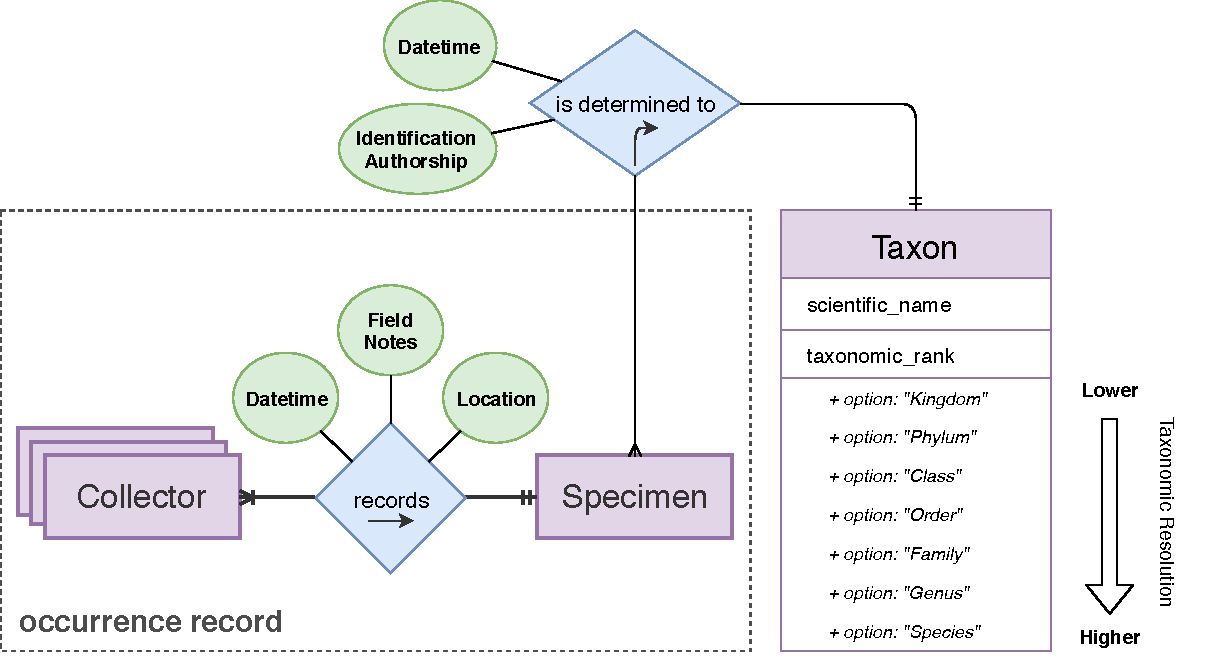
\includegraphics[width=\linewidth]{figures/collections_data/occurrences_er.pdf}
    \caption[Entity-relationship diagram illustrating the main features of occurrence records]{Entity-relationship diagram illustrating the main features of occurrence records. The cardinality of relationships is represented using the Crow's foot notation.}
    \label{fig:occurrences_er}
\end{figure}

\clearpage


Over the last 40 years, many institutions have adopted digital database management systems---or in the simplest cases, electronic spreadsheets---for improving the management and accessibility of their specimens-related data~\cite{Sunderland2013}.
Occurrence-related information is digitally stored in relational databases, while keeping references to the physical vouchers.
Each row corresponds to an occurrence, and includes contextual information such as the collectors' names, the geographic coordinates, date and time of the occurrence and the taxonomic identity of the recorded specimen.
Some initiatives~(\textit{e.g.} Reflora\footnote{\url{http://reflora.jbrj.gov.br}}) have also devoted significant effort towards the large-scale digitalization of physical specimens from biological collections, making high-resolution photos of the specimens digitally available for researchers.

One important upside of storing species occurrence information digitally is that institutions can more easily replicate and share their data with others, thus supporting wide ranges of applications using biodiversity information \cite{Newbold2010}.
Some data aggregation initiatives, such as the Global Biodiversity Information Facility (GBIF), have provided technological solutions for serving data from multiple collections to researchers through programmatic and visual interfaces \cite{gbif}.
In this context, it becomes relevant to represent data in an standardized and interchangeable format, such that records from distinct collections can be more seamlessly integrated.

Darwin Core (DwC)\footnote{\url{http://rs.tdwg.org/dwc/}} is a body of standards designed to provide a consistent vocabulary for representing biodiversity-related information and making it exchangeable, accessible, reusable and interoperable \cite{Wieczorek2012}.
An extension of the Dublin Core Metadata Initiative~(DCMI)\footnote{\url{http://dublincore.org}}, DwC has been specifically created and adopted as a standard for publishing biodiversity data, composed of many terms to designate \textit{classes} of entities and their \textit{properties}.
The \textit{Occurrence} class includes terms for representing many aspects of the gathering act \textit{per se}, documenting the existence of organisms at particular places and times.
Taxonomic information of organisms is represented under the \textit{Taxon} class.
Throughout this chapter, we refer to darwin core terms by prepending `\textit{dwc:}' to names (\textit{e.g.} the \textit{Occurrence} class becomes \textit{dwc:Occurrence} and the \textit{Taxon} class, \textit{dwc:Taxon}). \luiz{Tem também a classe {\em Event}, usada para amostragens periódicas, mas aí já foge um pouco de coleções biológicas, acho que pode deixar de fora. Talvez seja interessante mencionar que o futuro aponta para ontologias (p.ex. DOI:10.1371/journal.pone.0089606)}



% Species occurrence is not exclusive of biological collections Chapman2005b
%% Citizen science and informal collectors
% Hardisty2013
Last, it is worth noting that, although biological collections have been traditionally regarded as the main sources of species occurrence data, recent advances in mobile computing technology, associated with the increasing connectivity of electronic devices to the World Wide Web, have leveraged the participation of informal groups of nature observers towards recording and sharing biodiversity data in online platforms~\cite{Silvertown2009}.
Many of these communities also collaborate with researchers by sharing large amounts of records of their target organisms, in extents that would be otherwise impracticable to obtain, without enormous financial support.
The nature of such records is similar to those from biological collections in that they are punctual observations of specimens in nature, but also have some important distinctions.
First, nature observers usually materialize their observations through digital recordings~(audio, photo or video) instead of collecting physical biological samples.
The absence of physical specimens in many cases makes the identification of the observed organisms inaccurate, thus limiting the use of such data for scientific purposes.
In addition, identifications are often provided by a collaborative community of individuals with practical experience, not necessarily professional taxonomists and specialists.

\section{Limitations of data} 
\label{section:limitdata}
% Newbold2010 James2018 Hortal2007
% Presence vc presence-absence data
% Collectors Behavior (TerSteege2011)
% Limitations: sampling bias, lack of assessment of sampling effort, lack of geographic coverage
% Name ambiguity issue Groom2014

% Most species remain poorly collected , Nelson1990 TerSteege2011

% ===========
% Data issues
% -----------

Besides the remarkable relevance of biological collections as sources of biodiversity information, they are far from being adequate for investigating every aspect of natural systems.
This is partially a consequence of the fact that detailed information is unavailable or very scarce for most known organisms.
This scenario, referred to as the \textit{Wallacean Shortfall} \cite{Lomolino2004}, is even more critical for megadiverse countries, such as Brazil, which still remain largely unexplored for many regions and taxonomic groups \cite{Soberon2004}.
The lack of sufficient data for threatened species is even more concerning, as designing efficient programs for their conservation require knowledge on their geographic distribution and ecological requirements.
This shortage of data, combined with the non-systematic sampling and insufficient quality, limits the use of data from biological collections for many intended applications, many of which require an intensive amount of data to be available~\cite{Guisan2007}.
Failing to account for the inherent limitations of such data while posing and investigating their hypotheses, researchers may obtain erroneous or misleading results, eventually impacting the success of management policies that rely on such information \cite{Chapman2005}.
% Guisan2007 -> Many applications require high volumes of data, low sample size reduces the performance of many techniques
% Galante2017 -> Techniques for SDM using few records


\subsection{Sampling biases}
% charact. 2: Non-uniform sampling effort -> Lead to bias
One important aspect that often limits the usability of primary data from biological collections concerns the way in which it is gathered in the field.
In general, most species occurrence data composing biological collections derive from exploratory field expeditions, in which organisms are recorded in a non-systematic \textit{observational} fashion by different collectors, using different methods and at distinct circumstances (though records resulting from experimental studies are eventually incorporated in museums as well). 
As a result, the distribution of the sampling effort in such datasets is uneven and rarely quantified, leading to \textit{sampling biases}.

Building models without accounting for biases in data has been observed to strongly impact their performance, leading to spurious results which can be misinterpreted and, ultimately, lead to wrong decisions.
For instance, assessing patterns of species richness from species occurrence datasets has been shown to be particularly challenging due to geographical bias in data \cite{Hortal2007,Reddy2003}, as higher diversities tend to be observed at more accessible sites due to higher sampling effort.

As defined by \citeonline{Chrisman1991}, biases are uniform shifts in measured values, resulting from systematic errors that are introduced by some measurement system.
They are expressed as unrealistic tendencies in data, and can usually be mitigated with the adoption of random sampling designs.
%
Sampling bias in biodiversity data can be classified into several distinct categories, depending on the aspect of data under investigation \cite{Daru2017}.
Here we briefly present four of them, the first two (collector and taxonomic biases) being the most relevant in the scope of our work.
%
% collector bias, taxonomic bias, (geographic bias, trait bias, historical bias, seasonal bias) % Daru2017, Haripersaud2009 
\paragraph*{Collector bias.}
Not all collectors contribute to the same extent to biological collections.
In fact, it has been observed that a considerable percentage of records in biological collections are gathered by only a small subset of very productive collectors, while the vast majority of collectors contribute with just a few records each~\cite{Daru2017,Carine2012}.
This imbalance in the representativity of collectors is what defines the \textit{collector bias} in biological collections.
As the overall taxonomic composition of collections---as well as the geographical and temporal distribution of their records---tend to reflect the particular interests and collecting behavior of their most representative collectors, collector bias propagates to other categories of biases in the collection. Therefore, we consider that characterizing collector bias is a fundamental step towards understanding other types of biases.

\paragraph*{Taxonomic bias.}
Not all taxa are quantitatively represented in biological collections in the same proportions as they occur in natural systems.
Instead, the taxonomic composition of collections reflect the interests and collecting behavior of the communities of collectors contributing to them.
Moreover, rare species tend to be overrepresented in biological collections, as experienced collectors tend to prioritize collecting them over those which are more common \cite{Nelson1990}.
In addition, as collectors usually avoid collecting more than one exemplary of each species at the same place in a given expedition \cite{TerSteege2011}, common species tend to be underrepresented.
As the overall taxonomic composition of biological collections tend to reflect the interests and collecting behavior of their most productive collectors, taxonomic bias is intrinsically related to collector bias.
%
%Some studies have proposed to assess taxonomic bias of collectors by comparing the representativity of each taxon on their sets of records to the herbarium \cite{Haripersaud2009}. %Such approaches give at most a view of how well a collector represents the composition of the collection.
%However, if we consider the herbarium itself is composed of contributions of multiple collectors each with particular interests --- and therefore also biased ---, the herbarium is biased, not representing well the natural communities.
%As it is very common that collectors towards sampling the highest number of species as possible in localities they visit, the collection is non-random, and rare species tend to be overcollected and common species, undercollected \cite{TerSteege2011}.
%Biases of the most productive collectors would be hard to assess.

\paragraph*{Geographic bias.}
% [Kadmon, R., O. Farber, and A. Danin. 2004. Effect of roadside bias on the accuracy of predictive maps produced by bioclimatic models] 
Collection sites are not randomly selected in geographic space, nor they are all sampled to the same extent.
As features of the landscape make some areas more accessible for collection activities than others \cite{Hijmans2000}, collectors tend to prioritize those to maximize their productivity while minimizing costs.
Geographic bias thus arises as a consequence of non-uniform collecting effort in geographic space, and tends to reflect the preferred locations of the most productive collectors.
Some regions that are more accessible being thoroughly sampled (such as areas near urban centers, roadsides and margins of rivers);
while others that are more inaccessible, such as rainforests, being only poorly or not sampled at all.
%
Geographic bias is also observed at broader scales.
A compilation of the representativity of plants in GBIF by~\citeonline{Meyer2016} has shown that among the most representative countries and regions are the United States (mainly the west coast), Central America, countries in Europe (including the nordic countries), Australia, Japan, and New Zealand.


\paragraph*{Temporal bias.}
The patterns of the recording activities of collectors are not uniform over time.
Instead, collectors often show preferences towards performing field work in periods when they can get more productive, have more financial resources, or can find more organisms of their interests.
For instance, wet seasons possibly impact the performance of collectors in the field, and thus it would be natural to observe a relative drop on collecting activity during these periods.
Nevertheless, some organisms are better collected during wet periods~(such as \textit{Rivulidae} temporal fish), pushing collectors towards performing fieldwork despite unfavorable conditions.
Further, the availability of a naturalist for spending time in the field as a collector varies with their age, position, and stage in career.
While professional collectors would be available for collecting during weekdays, amateurs or students would be more available in weekends or vacation periods~\cite{Daru2017}.
The historical of records in biological collections therefore reflects the periods of activities of the most productive collectors.

% Two shortcomings: presence-only data and representativity


% Representativity
%Besides biases, another problem arising from non-uniform sampling effort concerns the representativity of species in biological collections.
%Collectors usually avoid collecting more than one exemplary of each species at the same place in the same expedition, and thus species representativity in museums do not correspond to their abundance in natural systems \cite{TerSteege2011}.
%In fact, rare species have been observed to be more represented than common ones due to the fact that more experienced collectors tend to prioritize collecting rare over common ones \cite{Nelson1990}.
%Moreover, non-uniform sampling effort hampers the assessment of species absences from `presence-only' occurrence data.
%As the sampling effort deployed over each location is usually not known for data in biological collections, the absence of a record for a species does not necessarily mean it does not occur there \cite{Graham2004}.
%Instead, it could be the case that no collectors who would potentially be interested on recording it have visited the location; or the species could not be detected at the time of the expedition.
% Problems in modeling
%Using presence-only data for assessing richness is problematic, although there are methods for overcoming this limitation, as most records available %for specimens are presence-only \cite{Zaniewski2002}.
%Richness was observed to be correlated to survey effort, richness is biased towards regions that are more thoroughly sampled \cite{Hortal2007}.

% Presence-only data and richness
%Non-uniform sampling effort also makes it hard to infer true absences from biological collection datasets.
%Species occurrence data is regarded as `presence-only', as they do not explicitly represent the absence of species.
%As the distribution of sampling effort towards locations is not known in biological collections, its data is regarded as `presence-only', which means that the absence of a record for a species at some location does not necessarily indicate that the species is truly absent \cite{Graham2004}.
%Instead, no collectors that would potentially be interested on recording it have visited the location.




% charact. 3: Data quality
% Briefly describe the limitations due to errors



\subsection{Data quality}
Besides biases, another important limitation in biological collection datasets concerns the \textit{quality} of data.
A definition for data quality (DQ) based on its \textit{fitness for the intended use} was first proposed in the context of geographical information systems \cite{Chrisman1984}, and became widely adopted by the BI community.
According to this definition, quality is not an absolute attribute of a dataset, but is rather given by its potential to provide users with valuable information, in specific contexts.
Assessing quality attributes of data is a fundamental step for any applications that might use it, and requires that users previously delimit the purpose, scope, and requirements of their investigation.
Data is considered to be of high quality if it is suitable for supporting a given investigation.
Depending on the application, users might need to improve the fitness of the data they have in hand, which is part of the data quality management process.

Loss of quality in biodiversity data can occur during multiple stages of its life cycle \cite{Chapman2005}, including the moment of the recording event, its preparation before it is incorporated in the collection, its documentation, digitalization, and storage.
% Include about data domains
Some of the most common problems are observed in the taxonomic and geospatial data domains, including the wrong identification of specimens, in part due to using outdated taxonomy; and bad georreferencing of records \cite{Soberon2004}.
In some cases, errors can be manually corrected by referring to supplementary information, such as the field notes of collectors \cite{Graham2004}.
However, this approach turns out impractical for large datasets, and methods for systematically assessing quality issues are required.


% Data problems
\citeonline{Dalcin2005,Veiga2014} have assessed the most common data quality issues in species occurrences datasets, and identified eight recurrent patterns of problems. %, observable across multiple data domains. 
During our study, we have identified five of them, which we considered to be most relevant:
(\textit{i})~\textbf{domain value redundancy}, when multiple distinct values in the dataset redundantly represent the same real-world entity;
(\textit{ii})~\textbf{non-atomic data values}, in case a value semantically contains multiple instances of the fundamental piece of information it should represent (an atomic value is regarded as being indivisible);
(\textit{iii})~\textbf{inconsistent data values}, in case they do not follow a strict standard, eventually leading to contradictory information;
(\textit{iv})~\textbf{incorrect data values}, when erroneous information are inserted in the dataset; and
(\textit{v})~\textbf{missing data value}, in case values at some field are absent (\textit{i.e.} null values).

A framework for systematically assessing and managing the ``fitness for use'' of biodiversity data from a user-centered perspective was recently proposed by \citeonline{KochVeiga2017}, and is based on three main components: \textbf{DQ Needs}, \textbf{DQ Solutions}, and \textbf{DQ Report}.
%
While defining DQ needs, users specify their \textit{use case}, comprising the main goals and scope of their investigation; the relevant \textit{information elements} that should be explicitly represented; and the \textit{dimensions} of data that should be assessed while measuring its quality.
Users also specify \textit{criteria} for defining acceptable measurements in each dimension; and activities for improving the suitability of data for the use case (\textit{enhancement}).
%
Within the scope of DQ solutions, users specify methods and implements tools for measuring, validating and enhancing data quality.
%
Finally, DQ reports are produced as documentations of the data quality assessment and management process in different contexts.
Users can therefore refer to such reports in order to evaluate whether their data is fit for their intended use, providing a basis for the collaborative development of data quality solutions (which authors refer to as a ``Fitness for Use Backbone'' (FFUB)).

\section{Data requirements for network modeling} % What should I do for improving data quality for SCN and CWN modeling
\label{section:datareq}
In this section, we briefly characterize aspects of data quality that are relevant for the network models presented in this dissertation.
Our models are constructed based on two \textbf{information elements}: the names of collectors and the taxonomic identity of the specimen at each occurrence record.
In a dataset following the DwC standards body, collector names and taxonomic identities should be found under the terms \textit{dwc:recordedBy} (class \textit{dwc:Occurrence}) and \textit{dwc:scientificName} (class \textit{dwc:Taxon}), respectively.
%
In SCNs, each record containing a set of collectors and a taxon. 
Interest ties are extracted from each record, linking each collector to the taxon.
More details on the construction process are provided in Section~\ref{subsec:scn-model-construction}.
%
In CWNs, only the collector field is required.
For each record, collaboration ties are created (or reinforced) by combining all collectors in a pairwise fashion.
More details of the construction process are provided in Section~\ref{section:cwn_construction_fromdata}.
%
Below we describe both information elements and highlight some of the main issues and requirements associated with them. 

% ========================================
% Information element: The collector field
% ----------------------------------------
\subsection{Collector names}\label{section:data_req_collector}
This information element contains the names of all collectors who were responsible for a species occurrence record.
From the field data domain \cite{Dalcin2005} \luiz{Essa frase ficou perdida ou não entendi}
In a DwC-compliant dataset, collectors names should be found under the term (or field) \textit{dwc:recordedBy} (within class \textit{dwc:Occurrence}), formatted as a list of collectors names concatenated into a string, using the vertical bar (` | ') as the delimiter.
For instance, a record authored by `M.A. Silva' and `N.T. Souza' would contain a string with value ``M.A. Silva | N.T. Souza''.
However, storing multiple names into a single string makes values in this field \textit{non-atomic}, thus requiring additional processing for the retrieval of individual names.

% names atomization
We refer to the process of extracting multiple names by splitting the string on a delimiter character as the \textbf{names atomization} \luiz{name atomization?} routine, which is mandatory for our use case.
Applying the names atomization \luiz{name atomization?} process to an entire dataset should be a trivial task if a consistent and non-conflicting delimiter (though not necessarily the vertical bar) is adopted throughout the entire dataset.
However, we suspect this is rarely the case for most species occurrence datasets.
Atomization issues arise when the atomization routine is unable to systematically distinguish names in a string, leading to the representation of unrealistic entities in the model.

% naming conventions
Using inconsistent (or ignoring) \textbf{naming conventions} while registering collectors names in a dataset is also potentially problematic, as it makes it more difficult to systematically interpret names and extract their component parts.
Naming conventions are rules used for shortening (or simplifying) names before they are inserted in the database.
One common practice is to abbreviate the first and middle names of collectors, while keeping the last name unabbreviated.
Under this convention, for instance, the name `João Souza Silva' would be mapped to `J.S. Silva'.
As collectors are not always aware of the naming convention adopted at the collection, they often include collectors names in their field notes using their own convention or, in the worse case, not using conventions at all.
The task to assure that all records are properly formated is therefore assigned to system managers, who must inspect and fix each entry manually before including them in the dataset.
As a result, names are eventually registered with typographical errors or being inconsistent with the adopted convention, although some database management systems are able to assist users in this aspect by parsing input names or by suggesting similar names that have already been registered.

% Heteronymous: result of inconsistent naming convention
Another negative effect of inconsistently formating collector names is the insertion of multiple \textbf{name variants} referring to the same real-world entity (domain value redundance).
This can also be the result of typos (e.g. souza becoming souza) \luiz{souza becoming sousa?}, or simply omitting parts of the name (e.g. if there are two collectors, A.~M.~Souza and A.~P.~Souza, omitting the middle initial makes their names indistinguishable).
%
The \textbf{entity-resolution} problem concerns the mapping of name variants that refer to the same real-world entity.
\citeonline{Groom2014} came across the same problematic, considerable variations in the formats of names.
They used a name cleaning routine in which they merged all variants of names that could be unambiguously mapped to a single person, while excluding those which could not.
This problem was also tackled by \citeonline{EstevaoDaSilva2016} by using a data mining methodology, based on association rules analysis, for identifying possible name variants.

% Homonymous
Assuming that all records in a dataset are consistent with some naming convention and that they use the same character for delimiting names (\textit{i.e.}, names can be properly atomized), distinct real-world entities may still end up being registered under the same name.
These entities, which we refer to as being \textbf{homonymous}, are also problematic for our use case, as they are incorrectly represented in the network models as a single entity.
In case the naming convention requires the abbreviation of parts of the names, homonymous can be created in the database from two names that are originally distinct.
For instance, `João Souza Silva' and `Jorge Soares Silva' would be mapped to a homonymous `J.S. Silva', if both the first and middle names were abbreviated.
%
Some collections include mechanisms in their naming conventions for disambiguating homonymous.
For instance, a complementary field containing unique identifiers for collectors can be appended to each record in the dataset, allowing the identification and resolution of homonymous entities.
Another approach would be making a
assigned to each for collectors can be included in the associated to each collector in the database management system, such that \luiz{frase não foi concluída}


% Omission
Finally, some collectors only include their own names in records in which they are first collectors, omitting the names of secondary collectors or, eventually, aggregating them under the expression `et al.'.
We refer to this issue as a \textbf{name omission} (within the \textit{completeness} DQ dimension), which strongly impacts as it fails to represent collaborative ties and collecting activities of the collectors who are not listed.

% Check Chapman2005a p.23

% ===================================
% Information element: The taxon name
% -----------------------------------
\subsection{Taxon name}
This information element contains the taxonomic identity assigned to the specimen from an occurrence record, being included into the taxonomic data domain.
In a DwC-compliant dataset, the taxonomic identities (or taxon) assigned to specimens at the highest resolution as possible are stored under the term \textit{dwc:scientificName}, which is part of the \textit{dwc:Taxon} class.
Other relevant elements within this class concern the common name of the taxon (\textit{dwc:vernacularName});
the rank of the taxon (\textit{dwc:taxonRank}); 
the names of higher-rank taxa within which the the taxon is classified (\textit{dwc:kingdom}, \textit{dwc:phylum}, \textit{dwc:order}, \textit{dwc:family}, \textit{dwc:genus}, \textit{dwc:specificEpithet});
the name of the author of the scientific name of the taxon\footnote{not to be confused with the author of the identification, in \textit{dwc:identifiedBy} (\textit{dwc:Identification} class).} (\textit{dwc:scientificNameAuthorship}).
%
Two important dimensions that possibly impact the fitness of taxonomic information for our use case concern the \textit{accuracy} and \textit{precision} of identifications; as well as \textit{misspelling errors}.

As exposed by \citeonline{Chapman2005a}, the \textbf{accuracy of taxonomic identifications} depends on the level of expertise of the professionals providing them.
For instance, a determination of taxonomic identity can be provided by the collector; by a professional taxonomist who is not an expert in the taxonomic group; or by a professional taxonomist who is either a regional or world specialist in that group.
Determinations provided by experts are, in general, more credible than those by non-experts, though even experts cannot always guarantee the highest degree of certainty on every identification.
Although information about the level of expertise of the determiners is typically not included in datasets from biological collections, many institutions adopt nomenclatural terms to convey the level of certainty in identifications, for instance `aff.' (for \textit{`affinis'}, suggesting affinity but not necessarily identity to other taxon) or `cf.' (for \textit{`confer'}, which is usually placed between the genus and epithet in the name of a species, indicating an uncertainty in the identification due to technical difficulties).

\textbf{Misspelling errors} are also included in the accuracy dimension of taxonomic data quality \cite{Veiga2014}, and are introduced in the datasets in a variety of ways, including typographic errors (typos), encoding issues, and from the incorrect transcription of names from how they sound \cite{Dalcin2005}.
Taxonomic authority files (files containing accepted taxonomic names) have been widely used for preventing the insertion of new invalid names during data entry; or for checking the validity of names already included in databases \cite{Chapman2005a}.
In addition, \citeonline{Dalcin2005} \luiz{o Taxamatch (DOI:10.1371/journal.pone.0107510) aprofundou as técnicas do Dalcin e ganhou o prêmio Ebbe Nielsen do GBIF em 2014, vale à pena adicionar a ref.} has proposed the use of both phonetic and string similarity algorithms for automatically screening potential spelling errors, by matching pairs of slightly different names with high degrees of similarity.

The \textbf{precision dimension of taxonomic data} is related to the most specific rank at which a specimen can be identified, \textit{i.e.}, its taxonomic resolution \cite{Veiga2014}.
Depending on the modeling requirements, a minimal taxonomic resolution may be necessary for the construction of the networks, making datasets more or less adequate for use.
Some applications using our models might require the representation of taxa at higher taxonomic resolutions  (\textit{e.g.} at the level of species), whereas for others it could suffice to use lower resolutions, such as the family level.
The precision of identifications is also related to the level of expertise of the determiners, although some groups of organisms are naturally more difficult to identify than others.
For instance, identifying mammals to the rank of species is far easier than insects.
Furthermore, higher levels of expertise are often required for identifying organisms within larger families, which comprise a higher number of species.
%
Therefore, assessing the proportion of records in a dataset that qualify for our network-based approach requires first defining the taxonomic resolution to be adopted during modeling.
In that sense, the \textbf{completeness of taxonomic information} (the proportion of records that are usable) is intrinsically associated with data precision.

Last, there are cases in which a taxon is referred to by to distinct names, although only one of them is accepted at any given time, according to the \textit{code of nomenclature} adopted.
Such names are said to be \textbf{synonyms}, and are an example of the domain value redundancy problem in the taxonomic data domain.
Similarly to redundancies in collector names, this issue leads to semantic inconsistencies in the network models (more especifically in SCNs), with entities represented more than once.
The insertion of synonyms in datasets can also be avoided during the data entry process, by using authority files based on the current code of nomenclature \cite{Veiga2014}. 













%% As it is common practice for botanists to record each species once during field work, some important ecological attributes such as the species abundance are not to be directly inferred from such data. {check van Gemerden 2005, from Haripersaud2009}


% Biological collections are composed of aggregates of multiple biodiversity surveys, each recorded with particular methodologies
% Records sampled using distinct methodologies can be combined for optimizing data use \cite{VanGemerden2005}.











% ============
% Data quality
% ------------
% [Soberon2004]

% Data quality among collection records is uneven -> worse for large datasets and for datasets composed by multiple sources
% Procedures are needed for correcting problems

% Quality issues: 
%% Determination issues: many specimens are incorrectly identified;
%% outdated taxonomy;
%% georreferencing errors.

% Data atomicity issues:
% Some fields are not atomic: more than one entity is represented as a single data element. 
% In the recordedBy field, Darwin Core standards state that distinct names should be separated by | (delimiter).
% This varies depending on the standard a collection uses. For example, the BRAHMS system recommends using a ';' as the delimiter.
% BRAHMS docs: https://herbaria.plants.ox.ac.uk/bol/brahms/support/documentation

% Identity issues:
% Entities are not guaranteed to have the same ids through distinct datasets.
% Even in the same datasets there may be variations in their names
% this is specially problematic for fields like the collectors field, which is overlooked for most applications of such data. 
% Some standards provide guidelines for including collectors names: last name + first initials...
% However different standards give distinct guidelines and thus name variants are common.
% How to map all name variants to the same entity? -> This leads to the Entity-resolution problem


% Data fit for use


% =============
% Data cleaning
% -------------
%[Chapman2005a]

% Why do we need data cleaning? -> We must make data fit for its indended use

% Goal: improving data quality, removing or treating entries that are 

% Adopting standardized collectors names
% Checking collectors itineraries -> look for the spatial pattern of records by the collector


% ================
% References
% ----------------
%% Museum-based informatics{Graham2004}




\chapter{Network Models}\label{chapter:network_models}


In this chapter, we present and formally describe two classes of network models that were developed during this study.
\textbf{Species-collectors networks} (SCNs) are built based on associations between collectors and the species they have recorded based on their field activities, whereas \textbf{collectors coworking networks} (CWNs) describe direct collaborative associations between collectors when recording specimens in field.

Although structurally distinct, SCNs and CWNs provide complementary perspectives on the recording behavior of collectors from a given species occurrence dataset. 
From SCNs, we retrieve information on which collectors have recorded which species and, conversely, which species were recorded by which collectors. 
On the other hand, CWNs allow us to investigate which collectors team up with whom during fieldwork, although here species are not represented as entities.
As both network models were elaborated based on a framework for social network analytics, we first review some general concepts from the network science and graph theory domains that are used in this study.

\art{Parei minha revisao aqui}

% ======================
% ======================
% Network Science Theory
% ----------------------

\section{Network Science: A theoretical background}

Network Science refers to a relatively new domain of scientific investigation, aiming to describe emergent properties and patterns from complex systems of interacting entities.
Such relational systems are naturally represented as networks, in which interactions are represented as pairwise connections (\textit{links}) between entities (\textit{nodes}) and assume particular semantics depending on the nature of the modeled phenomenon.
The rise of this field is strongly associated to recent advances of information technology, which provided scientists with novel tools for collecting, storing and processing data from many knowledge domains more efficiently and in larger scales.
Although a variety of networked systems in many disciplines had been studied long before that, technological advances allowed us to model real-world systems in much more details, from large volumes data that are often public or easily accessible for the investigator.

In a classic $1999$ paper which has inspired many researchers to engage into the field of network science, \textit{Albert-László Barabási}, \textit{Hawoong Jeong} and \textit{Réka Albert} built a model of the World-Wide Web from data collected by a web crawler \cite{Albert1999}. 
Their model represented the web as a set of interconnected documents, where a connection between document $a$ and document $b$ existed if either $a$ contained hyperlinks pointing to $b$ (outgoing links of $a$) or if $a$ was referred by $b$ through hyperlinks (incoming links of $a$).
By exploring some of the model topological features, they estimated that although the web is composed by a huge number of documents (by that time there were around $8 \times 10^8$ documents online), two randomly chosen documents are, in average, separated by as few as 19 links. 

Although surprising, this finding was in fact consistent with a generative model proposed by \textit{Watts} and \textit{Strogatz} in $1998$ \cite{Watts1998}.
In that paper authors argued that real-world networked systems are neither completely randomly nor completely regularly connected, and demonstrated that more realistic topologies could be derived by combining features from both extremes.
Following this approach they were able to generate network models which became known as the \textbf{small-world networks}, in which nodes are separated from others by very few connections, even for very large systems.
The name of the networks refers to a phenomenon known as the \textit{small-world}, which became popular after the experimental work of \textit{Stanley Milgram} \cite{Milgram1969} as the ``six degrees of separation''.
The concept referred to the finding that two arbitrary individuals in the world are separated by at most 6 connections, following an acquaintances chain.
 
Besides small-world networks, other models have been proposed in literature to explain mechanisms by which real world networks grow and acquire their particular topologies.
A \textit{preferential attachment mechanism} was proposed by \textit{Barabási} as ruling network growth by preferentially connecting new nodes to those in the network which already have many connections \cite{Albert2002}. 
This phenomenon is also referred to as ``the rich gets richer'' effect, and allows the appearance of few heavily connected nodes in the network, called \textit{hubs}. 
The majority of nodes in the network are, in contrast, very poorly connected, and thus unlikely to be linked to be included in new edges.
Networks with such characteristics are known as \textbf{scale-free networks}.

Those recently proposed models represent advances if compared to \textbf{random network models} introduced by \textit{Paul Erdos} and \textit{Alfred Rény} \cite{erdos1959random}, in which nodes are expected to connect to each other by chance, independently of the number of connections one already has.
According to \textit{Erdos} and \textit{Rény} $G(N,L)$ model, random networks are generated by creating $N$ distinct nodes and connecting them randomly and in a pairwise fashion with a total of $L$ links. 
If real-world networks behaved like random networks, topologies in which few hubs coexisted with a massive amount of very poorly connected nodes would be extremely unlikely to observe. 

Empirical results thus indicate that links are not randomly established in real-world networks.
Instead, a plenty of system-specific mechanisms occurring in smaller scales are thought to be key in the process of link creation.
Network growth is thus not governed by global mechanisms, but results from the orchestration of many local processes that occur between entities within the system.
We refer to such networks, in which non-trivial topological features emerge from the dynamics of subcomponents, as \textbf{complex networks}.
Uncovering some of such mechanisms and characterizing their effects in network topology compose the core of network science investigation.


%% Examples of networks in biology, computer science...
Network science has been applied to model networked systems in a variety of knowledge domains, including the internet, movie actors costarring networks, scientific collaboration networks, networks of human sexual contacts, cellular networks and ecological networks just to cite a few \cite{Albert2002}.
Given their relational structure, network models are formally represented as \textbf{graphs}.

Next we briefly review some fundamental definitions from \textit{graph theory}.
For the purpose of this work this is not intended to be a thorough review on the subject, but rather a quick overview for not familiarized readers. 
For a slightly more comprehensive introduction we recommend the reader to refer to \textit{Barabási}'s and \textit{Newman}'s books on network science \cite{Barabasibook,Newman2010b}.
In sequence we briefly describe the social network analytics framework and, 
finally, we give some examples of applications of network thinking in biodiversity literature.

% ============
% Graph Theory
% ------------
\subsection{General concepts on Graph theory}
\label{section:graphtheory}

Intuitively, \textbf{graphs} are mathematical structures composed by discrete objects holding pairwise connections to each other. 
In graph theory terminology, objects are referred to as \textit{vertices} and the connections between them as \textit{edges}.
Graph structure provides a natural representation for networked systems for a couple of reasons.
First, they allow representing entities and their interactions in a structured way, as a ``map of connections'' through which information flows.
Second, graph theory provides a bunch of well established data structures, metrics and algorithms for systematically representing, characterizing and exploring the topologies of complex networks.
Finally, the availability of a considerable amount of graph visualization tools and techniques helps analysts to obtain insights from network structure, by allowing them to focus on different aspects of the system depending on their own interests.

% Graph formal definition, undirected/weighted graphs
A graph is formally defined as a pair $G=(S,E)$, where $S$ is the set of vertices and $E$ is the set of edges that compose it (Figure \ref{fig:graphs}). 
%
Edges necessarily involve pairs of vertices, and are thus represented as $(u,v)$, for $u,v \in S$.
Pairs of vertices that are directly connected by an edge are said to be \textit{adjacent}, and the set of all vertices that are adjacent to a given vertex composes its \textit{neighborhood}.
%
Depending on the nature of the modeled connections, edges can be either classified as \textit{undirected} or \textit{directed}.
Undirected edges model symmetric connections, in which case information is allowed to flow equally in both directions.
There are situations, however, in which information necessarily flows from a source to a target vertex, thus making connections asymmetric.
Those are represented in the graph as directed edges.
Graphs strictly composed by directed edges are known as \textit{digraphs} (or \textit{directed graphs}), whilst \textit{undirected graphs} only have undirected edges.
In undirected graphs we should note that edges $(u,v)$ and $(v,u)$ are equivalent.
%
Additionally, connections in a networked system can be modeled as either being all identical or distinct in terms of their strengthness or relevance, which is incorporated in the graph as edges \textit{weight}.
Graphs are also classified regarding the nature of their edges.
A graph in which all edges are weighted is known as a \textit{weighted graph}, whilst a \textit{unweighted graph} is exclusively composed by unweighted edges.
%
Given the nature of the networks modeled in the context of this project, we specifically focus on properties of \textbf{undirected weighted graphs} for the rest of this section.

  \begin{figure}[h!]
  	\centering
    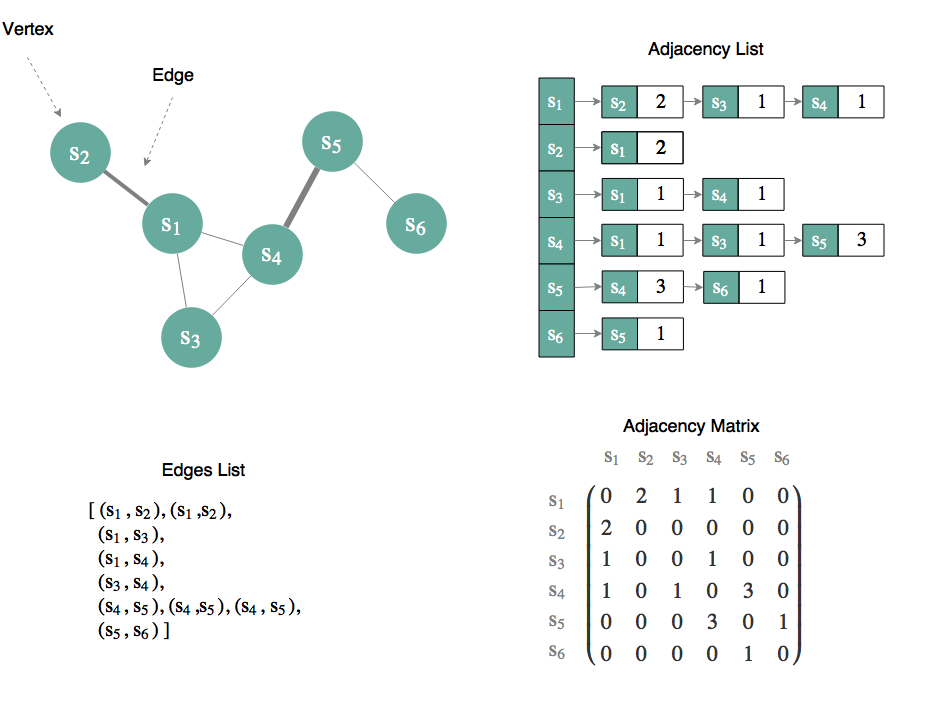
\includegraphics[width=0.9\linewidth]{figures/network_models/graphs.png}
    \caption{Undirected weighted graph with six vertices and six edges; and three of its possible representations.}
    \label{fig:graphs}
  \end{figure}
  
\textit{Attributes} allow representing non-topological features that are relevant in the context of the modeled system, and can be optionally assigned to both edges and vertices in a graph.
For example, we might want to model a social network in which individuals name, age and gender information are relevant for our analyses.
Such features, which assume distinct values for each individual in the network, are typically stored as vertices attributes.
Similarly, edges attributes store particularities regarding each individual connection.
In thesis, any numerical attribute could be used for edges weighting.

% Graph representations
Graphs can be computationally represented using a variety of data structures, the most appropriate one heavily depending on the set of algorithms one expects to run against the graph.
Here we present the three most common of them (Figure \ref{fig:graphs}).
%
\textit{Edges lists} are perhaps the simplest and most intuitive graph representation, and consists of a list storing all edges as ordered pairs $(u,v)$, for $u,v \in S$.
Given its simplicity, this representation is more appropriate for situations in which the user directly interacts with the data, such as when manually creating or editing graphs without the aid of specialized software. 
This representation is also compact enough to be adopted for graph storage and data exchange in some situations.
%
Most algorithms, however, perform better by using alternative designs such as \textit{adjacency lists} or \textit{adjacency matrices}. 



\textbf{Adjacency matrices} are a way to represent graphs in matrix form, in which elements store adjacencies between pairs of vertices.
An adjacency matrix $A$ is defined as having non-zero entries $a_{i j}$\textit{ iff } $(i,j)\in E$ which, in weighted graphs, correspond to the weight assigned to edge $(i,j)$.
Given the equivalence between edges $(i,j)$ and $(j,i)$ in undirected graphs, adjacency matrices in this case are always symmetric, meaning information is stored redundantly in its structure.
%
Besides, the size of an adjacency matrix grows quadratically with the number of vertices in the graph, which would make loading and processing large graphs in computer memory problematic.
However, real-world networks have been observed to be naturally sparse, meaning that only a very small percentage of all possible edges do in fact exist.
Adjacency matrices can thus be optimized for storage and performance by adopting standard sparse matrix representations such as compressed row storage (CRS) \cite{Saad2003}.
An alternative way to represent sparse networks is to use the \textit{adjacency list} representation, which in short consists of storing a list of neighbors for every single vertex in the network. 
The adjacency list illustrated in Figure \ref{fig:graphs} is structured as an array for which each entry represents a vertex.
Moreover, each entry holds a reference for a linked list, containing all neighbors of the vertex. Each element in the list keeps a reference to the next element and stores the weight of the edge connecting it to the vertex in the array.

% Definitions and metrics
As previously mentioned, one of the main benefits of adopting graphs for representing networks is the availability of a whole set of well-established metrics and definitions that allow analysts to explore and characterize the topologies of their networked systems.
Below we review some of the most basic ones.

\paragraph*{Path.}
A path can be thought of as a chain of adjacent vertices composing a route through which information flows in a graph.
For undirected graphs we say there exists a \textit{path} of length $n$ between a pair of vertices if they are mutually reachable by following a sequence of $n$ edges.
Pairs of vertices are said to be \textit{connected} if at least one path exists between them, the shortest of which being defined as their \textit{distance}.
A graph can be described in terms of its \textit{average path length}, which is computed by averaging the path lengths between all pairs of connected vertices.
Finally, the \textit{diameter} of a graph is given by the greatest distance between any pair of vertices composing it.

\paragraph*{Connected component.}
A connected component is a subset of vertices in the graph in which all included vertices are \textit{connected} to every other one by at least one path.
Moreover, this subset is required to be maximal, meaning that all vertices in the network for which the inclusion property holds should also be included in the component. 
A graph can be composed by many distinct connected components completely disconnected from each other, the largest of which is called the \textbf{giant component}.

\paragraph*{Clique.}
A clique is a structure composed by a subset of vertices in which all included vertices are \textit{adjacent} to each other.
The set of edges that compose a clique are obtained by computing the pairwise combination of all its $n$ vertices, being the total number of edges in the clique given by the binomial coefficient $\binom{n}{2}$.

\paragraph*{Density.}
Density is one of the simplest metrics for assessing graph connectivity, and indicates the proportion of pairs of vertices that are connected by edges.
For a graph with $n$ vertices density is given by $\frac{2E}{n(n-1)}$, where $E$ is the number of edges in the graph.
Possible values for density are thus bound from $0$ to $1$, where $1$ is obtained for a \textit{complete graph} (or a \textit{clique}) and $0$ would be obtained for a graph with no edges.
This concept is the inverse of graph \textit{sparsity}. 

\paragraph*{Clustering.}
Density alone is seldom a sufficient metric for investigating relevant patterns of connectivity in real-world networks, as they their topologies usually display \textit{clustering patterns}.
\textit{Clusters} are regions in the graph within which vertices are signifficantly more densely connected than average and more loosely connected with other vertices from the rest of the graph. 
Clustering analysis is particularly useful in the context of social networks analysis for identifying communities.
%
\textit{Clustering coefficients} can be used to characterize the level to which vertices are clustered in a graph, and can be defined as either local or global metrics.
The local clustering metric $c_i$ for a given vertex $i$ is calculated by evaluating how close to a clique is a subgraph composed by itself and all its $k$ neighbors (which is known as the \textit{ego network} of vertex $i$). Thus, $c_i = \frac{2L_i}{k_i(k_i - 1)}$, where $L_i$ is the number of edges connected to $i$ and $k_i$ is the degree of $i$.
To illustrate with an inutitive example within the context of social networks, clustering coefficient is an answer to the question ``How many of my friends are also friends themselves?''.
%
The global clustering metric $c_{\Delta}$, on the other hand, computes the fraction of triples in the graph that compose cliques (or triangles).In short, \begin{equation}\label{eq:globalclustering}
c_{\Delta} = \frac{3 \times numOfTriangles}{numOfTriples}
\end{equation}

%% Transitivity
\paragraph*{Transitivity.}
The transitivity relation for a triple of nodes $\{a,b,c\}$ is observed if the fact that node $a$ is connected to $b$ and $b$ to $c$ implies that $a$ is connected to $c$.
In social networks terms, this relation represents the phenomenon that ``a friend of my friend is also my friend''.
Network transitivity is often used as a synonym for \textit{clustering}, and thus the overall transitivity of a network can be quantified through the global clustering coefficient from equation \ref{eq:globalclustering}.



\paragraph*{Degree.}
The degree (denoted $k$) of a vertex in a undirected graph is given by the total number of vertices that are adjacent to it or, in other words, the length of its neighborhood.
We compute the degree of a particular vertex $i$ from the graph's adjacency matrix $A$ as 
$
k_i = \sum_j bool(a_{i j})
$,
where $a_{i j}$ are elements containing the weights of each edge $(i,j)$; and the function $bool$ evaluates to $1$ if the element is greater than zero and $0$ otherwise.
We can similarly compute the \textit{weighted degree} for vertex $i$ as $ k_w^{(i)} = \sum_j a_{i j} $.
The \textit{average degree} 
$\langle k \rangle$ 
is a global property of the network, computed by averaging the degree values for each individual vertex $i$:
$\langle k \rangle = \frac{1}{N} \sum_{i=1}^N k_i$.

\paragraph*{Degree distribution.}
The probability distribution of vertices degrees over a graph is known as its \textit{degree distribution}.
From degree distribution we retrieve the probability $p_k$ that a randomly selected vertex from the graph has degree equal to $k$.
In random graphs degree distribution is typically well approximated by a poisson model, which peaks at $\langle k \rangle$.
Thus vertices with degree equal $\langle k \rangle$ are most likely to occur, whereas those with very high and very low degrees are very unlikely. 
As mentioned in the previous section, however, most real-world networks are majoritarily composed by low-degree nodes, coexisting with few hubs.
Such a scenario is better described by a \textit{power law}, such that $p(k) \sim k^{-\alpha}$.

\paragraph*{Degree correlation.}
A graph shows degree correlation if vertices degree determines the degrees of its neighbors with a certain magnitude.
A positive correlation indicates that edges are more likely to connect pairs of either high-degree or low-degree vertices.
On the other hand, a negative correlation indicates that connections are more likely to exist between high-degree and low-degree vertices.
A variety of metrics have been proposed in literature for assessing degree correlation in a graph \cite{Newman2003b}, being the \textit{Pearson correlation coefficient} one of the most widely used.
Generally, correlation values range from $-1$ for maximal negative correlation; to $1$ for maximal positive correlation. 

\paragraph*{Mixing patterns.}
Mixing patterns describe the effects of nodes characteristics on influencing links formation in networks.
In case associations are more likely to establish between nodes which are similar on some characteristic, the pattern is known as \textit{assortative mixing} or, in social sciences, \textit{homophyly}.
In contrast, \textit{dissortative mixing} is observed when nodes preferentially connect to others with opposite characteristics. 
If nodes characteristics show no signifficant influence on links formation, we say the network is \textit{neutral}.
Degree correlation can be understood as a specific type of mixing pattern, evaluated on vertices degrees.

\paragraph*{Centrality.}
Centrality analysis concerns the identification of influential entities in the network, who might assume important roles in the system under different perspectives.
\textit{Degree centrality} is perhaps the simplest centrality measure, and assumes that the relevance of a node only depends on its own degree. Nodes with many connections are thus more influential than those with fewer connections.
If we consider, however, that the relevance of a node also depends on the relative importances of their neighbors (and that some neighbors are more influential than others), the \textit{eigenvector centrality} becomes a more realistic metric \cite{Bonacich1987}.
In this case nodes holding fewer links to more influential ones might turn out to be more influential than those holding more links to less influential nodes.
Other centrality metrics emphasize the importance of other topological aspects instead of node degree.
\textit{Closeness centrality} measures the importance of a node by computing its mean distance to all other nodes in the network, and thus nodes are more influential if they can reach their peers more efficiently by taking shorter paths.
\textit{Betweeness centrality} identifies nodes which are important strategical intermediators, if they are included in the path between many pairs of nodes in the network.  

\paragraph*{Bipartite graphs.}
Bipartite graphs, also known as bigraphs or two-mode graphs, are a special class of graphs composed by two distinct sets of vertices $U$ and $V$, with the constraint that no vertices within the same set are allowed to be adjacent to each other. 
We define bipartite graphs as triples 
$
B = (U, V, E) \mbox{, }
$
where $E$ is the set of edges between vertices from $U$ and $V$.
Using sets theory terms, $U$ and $V$ are both \textit{disjoint} and \textit{independent} sets.
This means vertices must be assigned to exactly one vertices set and, moreover, all edges in $E$ necessarily connect vertices from opposite sets. 
Such features make bipartite graphs particularly useful for representing interactions that only make sense to exist between entities of different classes. 

  \begin{figure}[h!]
  	\centering
    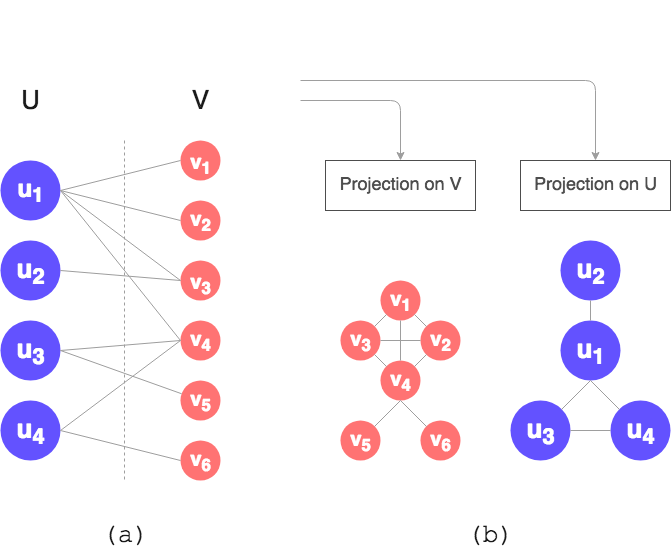
\includegraphics[width=0.5\linewidth]{figures/bipartite_general.png}
    \caption{General aspect of a bipartite graph (a). All vertices in the graph belong to exactly one of $U$ and $V$ vertices sets. In addition edges are only established between vertices from distinct sets. (b) Bipartite projections. Projections onto each node set are constructed by linking together vertices that are at a length-2 distance in the bipartite graph, while omitting vertices from the opposite set.}
    \label{fig:bipartite_general}
  \end{figure}

%% Biadjacency matrix
The \textit{biadjacency matrix} (or \textit{incidence matrix}) is the matrix representation of a bipartite graph, being equivalent to adjacency matrices defined for one-mode graphs (those composed by a unique vertices set). 
Differently from one-mode graphs for which the adjacency matrix is necessarily square, biadjacency matrices are usually rectangular, unless both vertices sets have the same size.

%% Bipartite projection
As most algorithms and metrics in literature are primarily designed for one-mode graphs, it is often convenient to summarize a bipartite graph by directly linking vertices that belong to the same set based on indirect associations they might have. 
This operation, in which vertices from one set get directly linked if they are intermediated by at least one vertex from the opposite set, is called a \textit{bipartite projection} (Figure \ref{fig:bipartite_general}b).
Projections thus compress a bipartite graph into a one-mode graph by only representing vertices from the projected set, while those from the opposite set are omitted.
Therefore, bipartite projections into each vertices set provide complementary perspectives on the relationships modeled.
%




% ===============
% Social Networks
% ---------------
% Mark Granovetter paper (1973)
%% Which types of analyses are most common in social networks?

\subsection{The Social Network Analytics framework}
In the context of this work we refer to the \textit{social networks analytics framework} as a set of concepts, methods and algorithms which can be directly applied or slightly adapted for modeling and analyzing social networks in diverse and independent contexts and knowledge domains.
%
In our definition, we refer to \textit{social networks} as systems in which entities (mostly people) interact with each other through some type of \textit{social tie}.

As social networks are themselves a particular class of networks, most of the theoretical foundation used to study them is directly inherited from network science.
%
Social networks, however, display two important particularities if compared to other types of networked systems \cite{Newman2003d}.
First, entities tend to organize themselves in groups within social systems, such that those who are members of the same group tend to interact more intensely with themselves than with non-members.
This contributes to the formation of communitites structures, making social networks \textit{highly clustered}.
Second, as entities belonging to larger groups tend to interact with many peers --- and, conversely, entities belonging to smaller groups tend to interact with fewer peers ---, social networks tend to be assortatively mixed, in contrast with non-social networks which are typically disassortative.  

%Properties 
A variety of social network models within many distinct areas have been proposed in literature.
Most authors have primarily focused on obtaining domain-specific insights from statistical and topological properties of network models such as \textit{degree distribution}, \textit{degree correlation}, \textit{mixing patterns}, \textit{nodes centrality} and \textit{clustering} \cite{Newman2003b}.
Next we describe some of them for giving the reader a more solid intuition on how they're structured before we introduce our own models.


% Affiliation networks
\textbf{Affiliation networks} are a particular type of social networks in which individuals are associated to events, groups or institutions (we'll refer to all those as organizations) by being members or participating in them \cite{Borgatti2015}. 
%
Such networks are considered relevant in the context of social networks analytics due to the fact that individuals belonging to the same groups or attending the same events are more likely to become acquainted and develop social ties than those who are not affiliated to common organizations.
%
The most conservative way to structure affiliation networks, so that we keep the complete information on who have affiliated to which organizations, is achieved by representing both individuals and organizations as distinct types of entities in a bipartite model.
 
A classic example of affiliation networks is the movie actors network, introduced as an empirical example in \textit{Watts} and \textit{Strogratz}'s work \cite{Watts1998} while describing the small-world property in real-world networks.
This network was built from the Internet Movie Database (IMDB \footnote{\url{http://www.imdb.com/}}), by linking actors to movies they have starred in.
Actors and movies are thus modeled as distinct entities in the network, such that an actor gets connected to all movies he/she has participated in, whilst a movie gets connected to all actors who have composed its cast.  
From complementary perspectives, one could distinguish for instance movies that are most similar in terms of their cast composition and, on the other hand, actors that are most related by having starred in the same sets of movies.
%
Similarly, \textit{Davis}, \textit{Garder} and \textit{Gardner} have studied women social circles from data on their attendance to public social events, and related how their attendance behavior could be influenced by their own social casts \cite{Davis1941a}. 

Another well-known application of affiliation networks are scientific papers authorship networks, in which authors get connected to papers they've authored.
In this case, however, the focus has been mostly on deriving co-authorship relationships between paper authors, and in many cases the individual papers which originated the co-authorships are not very relevant \cite{Newman2004, Borrett2014}.
A simplified one-mode network, in which only authors are represented as nodes and get directly linked by co-authorship relations, can be derived from the bipartite model by computing its projection onto the authors nodes set.
In the resulting network, authors who have collaborated at least once in paper production get directly connected.
Networks where edges assume this semantic are also known as \textbf{collaboration networks} (or, alternatively, \textit{coworking networks}) \cite{Ramasco2004}.
They can either be directly constructed from data or be obtained by projecting affiliation networks.

Apart from affiliation networks, the bipartite structure is also suitable for modeling other types of social networks.
One of those, which we here refer to as \textbf{interest networks}, model relations of interest from entities towards objects.
Besides their structural similarity to affiliation networks, relationships modeled in interest networks are conceptually distinct from the former, as the fact of two individuals sharing interests does not necessarily provide them differentiated opportunities for developing social ties.
Instead, interest networks tie together individuals with objects they're interested in, independently of the social groups or communities they are members of. 
Thus, instead of social communites, interest networks are more appropriate for revealing {\textit{communities of interests}.
%
Interest networks have been used for instance to characterize collective music listening habitats among users of media streaming platforms \cite{Lambiotte2005}.
From a network of listeners interests towards music groups, \textit{Lambiotte} found evidence that the traditional music genres classification by the music industry is not the best way to categorize listeners in terms of their listening behaviors.



% ========================
% Networks in Biodiversity
% ------------------------
\subsection{Networks in Biodiversity}
Network modeling has been widely adopted in the context of biodiversity research, especially for investigating ecological and evolutionary aspects of ecosystems and natural communities. 
Efforts towards this goal have led to the creation of the field of \textit{network ecology}, which has undergone a noticeable growth over the last few years \cite{Borrett2014}.
% Interaction networks
Network ecology has traditionally focused on describing general aspects of the entangled networks by which organisms interact.
As ecological interactions are regarded as key processes modeling ecosystems functioning and structure, unraveling their architecture and dynamics is detrimental for understanding a variety of ecosystem features, such as stability and energy flow.
%
Interaction networks can be broadly classified as \textit{food webs}, \textit{host-parasitoid webs} or \textit{mutualistic webs} \cite{Ings2009}, being food webs the first ones described in literature, since two classical papers by \textit{Lindeman} and \textit{Odum} \cite{lindeman1942trophic, odum1956primary}. 
%

%Animal movements
Besides ecological interactions, network thinking has also been applied for modeling other aspects of natural systems.
Patterns of animal movement can be investigated in a structured way, for instance, by means of \textit{movement networks} \cite{Jacoby2016a}.
These networks represent geographical space as a set of discrete and interconnected locations, forming a mesh of possible routes through which animals (or groups of animals) transitate. 
Links between each pair of locations are weighted according to their geographical connectivity.
Animal movement is thus regarded as dynamic processes composed by sequences of discrete movement steps running through the network structure.
As the spatial feature is key in this type of network, they are also referred to as \textit{spatial networks} \cite{Bascompte2007}.
%

%%% Co-occurrence networks 
Others have applied network science to investigate biogeographical patterns, such as species co-occurrence. 
So called \textit{co-occurrence networks} model species associations in terms of their geographical distributions, such that species which are often observed occurring together in the same set of localities are considered to be strongly associated.
Similarly to other networked systems, co-occurrence networks are composed by a majority of the species holding co-occurrence links to very few others, whilst only few species are connected to many others \cite{Araujo2011a}.
Co-occurrence network analysis has been used for many applications, including for selecting subsets of species to be used as surrogates for the characterization of biological communities \cite{Tulloch2016};
for assessing the resilience of biotic communities towards climate change \cite{Araujo2011a};
and for identifying modularity (clusters of overlapping species ranges) in biological communities from animal-location bipartite networks \cite{Thebault2013}.
%%% Challenge: Reliable data is hard to be obtained


% Social Networks and Biodiversity
The social network analytics framework has also been applied in some biodiversity studies, though in most cases for modeling animal social behavior \cite{faust2011animal}.
An alternative perspective is to look at communities of biodiversity data producers and consumers, in order to better understand the myriad of contexts in which data is collected, shared and used.
%
Mapping data flow within the community of biodiversity informatics initiatives, for instance, could help prioritizing and improving the coordination of collaborative actions, leading to more effective biodiversity data-based policies \cite{Bingham2017}.
%
Also, important scientific communities and gaps could be identified and characterized by exploring collaborative paper authoring networks and scientific topics networks \cite{Borrett2014}. 
%
Another interesting example of a collaboration network in biodiversity is given in \textit{Groom`s} work, where a correspondence network of $19th$-$20th$ century botanists was structured from digitized data from the British Herbaria \cite{Groom2014}.
Botanists composing this network corresponded to each other by exchanging specimens, a practice that has led to the formation of exchange clubs.
Many aspects regarding the particular ways botanists used to work as well as the roles they assumed could be investigated with the aid of exchange networks 

% TODO Is this the best way to place this paragraph?
Finally, a better understanding of the factors and processes influencing the composition of species occurrence datasets would be invaluable for improving data usability, especially for species distribution modeling \cite{Daru2017}.
As biological collections are typically composed by an ensemble of opportunistic species occurrence records, each of which having been gathered in a particular context by a different collectors team, their datasets do not necessarily reflect the biological diversity from the area within which the collections are physically located.
Rather, they best reflect the interests of their most relevant collectors, those who have contributed to the collection to greater extents. 
%
In our work we understand the assemblage of a species occurrence dataset as a social process, resulting from a multitude of complex interactions between individual collectors, each of them having particular preferences towards recording taxonomic groups and collaborating with other collectors.
The network models we propose in the following section help characterizing collectors in terms of their interests and recording behavior, as a proxy for a better understanding on the assemblage of biological collections.
  




% ===========================
% ===========================
% Species-collectors Networks
% ---------------------------

\section{Species-collectors Networks}

In this section we introduce species-collectors networks (SCNs) as modeling associations between collectors and species they record. 
We first give an overview on the semantics of the modeled relationships and provide a formal definition of SCNs using graph theory.
Then, we describe how such networks can be built from species occurrence datasets.
Finally, we define attributes and operations for SCNs that facilitate obtaining domain-specific insights from network structure.

\subsection{General Description}
%% Model semantics
\textbf{Species-collectors networks} are a particular type of \textit{interest networks} describing relationships of type ``\textbf{collector} samples \textbf{species}'' or, conversely, ``\textbf{species} is sampled by \textbf{collector}'' (Figure \ref{fig:scn_general}). 
The network is thus composed by collectors holding links to every single species they have ever recorded or alternatively, species holding links to every collector who have ever recorded them.
An important semantic aspect of this model worth emphasizing is that here we model collectors recording \textit{species} rather than \textit{specimens}. 
As exposed elsewhere in this text, the term \textit{species} refers to a grouping of individuals (or \textit{specimens}) which share a set of features and are thus considered to be taxonomically equivalent at that level. % TODO : substitute 'elsewhere' by the section ref
Each occurrence record that is used to build the network includes a single specimen, which is a representative of a species.
Thus, while collectors are represented in the network at the individual level (each collector is a person), species are instead represented as entities comprising groups of individuals.
Nevertheless each species is uniquely represented as a node in the network.

  \begin{figure}[h!]
  	\centering
    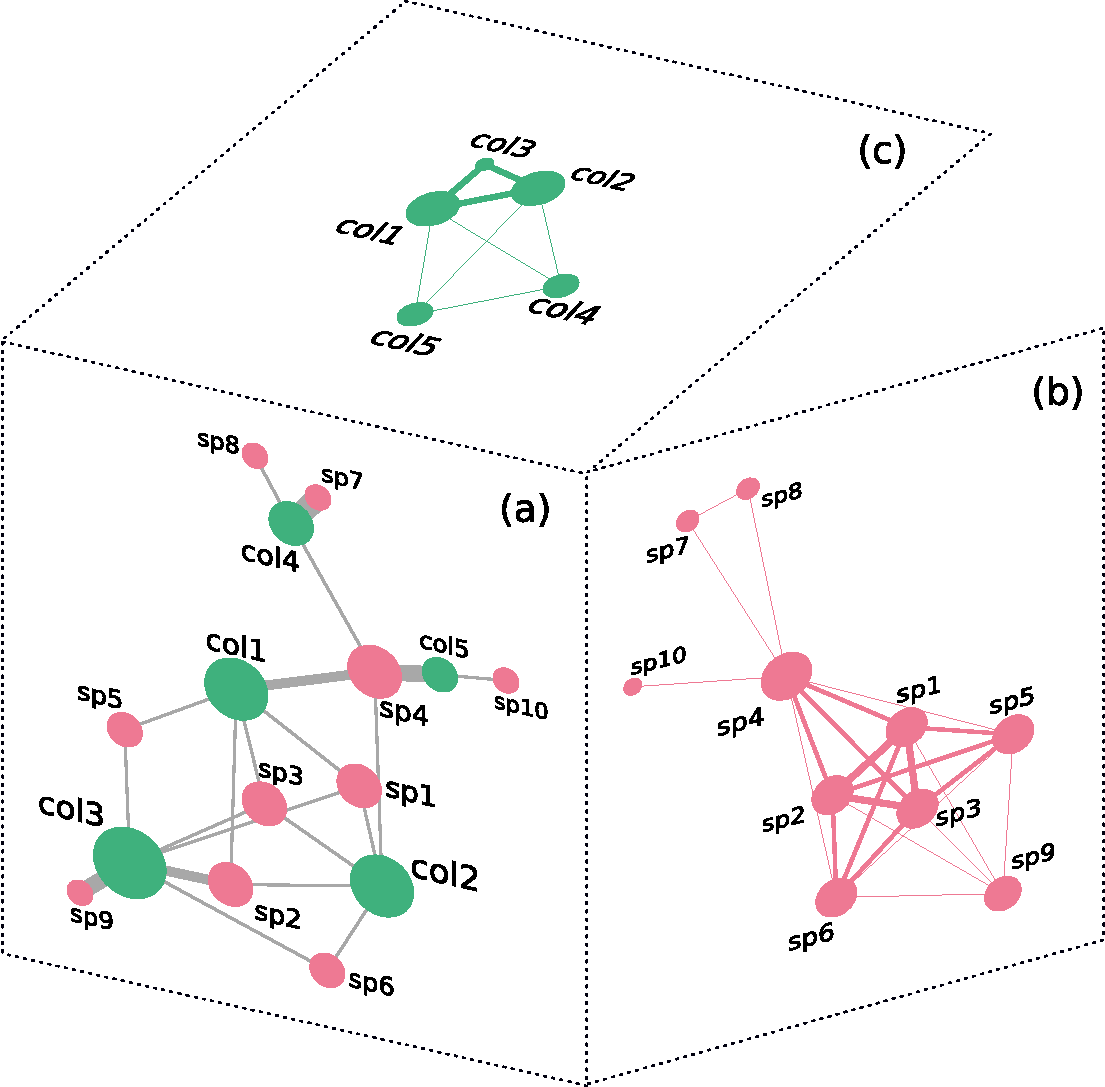
\includegraphics[width=.7\linewidth]{figures/network_models/scn_generalaspect.pdf}
    \caption{Multiple perspectives of a Species-collectors Network model (SCN).
    (a) Unprojected network, where collectors (green nodes) are linked to the species (red nodes) they've recorded. The total number of records of a given species by some collector is reflected in the strength of their link. (b) SCN projection onto the species set. Species are linked together if they've been collected by common collectors. Link strength is proportional to the number of collectors two species share. (c) SCN projection onto the collectors set. Collectors are linked together if they've recorded species in common. Link strength is proportional to the number of species two collectors share. 
    Link strength for both projections were obtained using the \textit{simple weighting} rule (eq. \ref{eq:simple_weighting}), and are graphically displayed as edges thickness. Nodes sizes reflect collectors' and species' degrees in each perspective.}
    \label{fig:scn_general}
  \end{figure}
  
%% Model specification
As collectors and species refer to distinct entities in our system, we represent them in our network as two disjoint nodes sets.
Moreover, as interest relationships here modeled can only possibly exist between collectors and species we impose an additional constraint that all edges in the network must necessarily connect nodes from distinct sets.
This best matches the description of a bipartite network
$$ SCN = (S_{col},S_{sp},E) \mbox{ ,}$$
where $S_{col} = \{u_1, u_2, ..., u_n \}$ is the nodes set representing the collectors group; $S_{sp}=\{v_1,v_2, ..., v_m\}$ is the nodes set representing the species group; and $E$ is the set of undirected edges between members of $S_{col}$ and $S_{sp}$.
The bipartite graph can also be represented as a rectangular biadjacency matrix $A^{n\times m}$ for which $a_{ij}\neq 0$ \textit{iff} $(u_i,v_j) \in E$. Values of non-zero $a_{ij}$ elements are set to the number of times edges $(u_i,v_j)$ occur in the network, as described below. 
For a general overview of bipartite graphs the reader should refer to section \ref{section:graphtheory}.

  
%% Network construction
\subsection{Model construction from data}
A SCN model is built from a species occurrence dataset by using basically two fields.
The first is the collectors field, containing the names of all collectors that were responsible for the record; and the second is the species field, storing the species identity assigned to the specimen in the record.
Following Darwin Core terms standard\footnote{\url{http://rs.tdwg.org/dwc/terms/}}, we should expect to find collectors names in the \textit{recordedBy} field; and the species name in a field named \textit{species}. As not every biological collection dataset uses Darwin Core standards though, these fields might be occasionally found under different names.

The network is built up from the dataset in an iterative process, in which weighted edges linking collectors to species are structured from rows in the dataset.
For each new record containing $n$ collectors, $n$ links connecting each individual collector to the recorded species are created (or strengthened, in case they already existed).
In the end of the process, the strength of each link is equivalent to the number of times each association appears in the original dataset.
The more often a particular collector records a particular species, the stronger gets the link between them.
Moreover, as at least one additional link is necessarily either created or reinforced for each new row, the construction process guarantees that no disconnected species or collector nodes can possibly exist in a species-collectors network.
For a concrete example, the dataset used for creating Figure \ref{fig:scn_general} is given in Table \ref{table:scn_example_dataset}.

\begin{table}[!ht]
  \caption{Species occurrence dataset from which the SCN model in Figure \ref{fig:scn_general} was built.}
  \begin{center}
  \begin{tabular}{r l c}
      id & recordedBy & species \\
      \hline
      0 & col1; col2; col3 & sp1 \\
      1 & col1; col2; col3 & sp2 \\
      2 & col1; col2; col3 & sp3 \\
      3 & col1; col2 & sp4 \\
      4 & col1 & sp4 \\
      5 & col1; col3 & sp5 \\
      6 & col3; col2 & sp6 \\
      7 & col3 & sp2 \\
      8 & col4 & sp4 \\
      9 & col4 & sp7 \\
      10 & col4 & sp7 \\
      11 & col4 & sp7 \\
      12 & col4 & sp7 \\
      13 & col4 & sp8 \\
      14 & col3 & sp9 \\
      15 & col3 & sp9 \\
      16 & col3 & sp9 \\
      17 & col5 & sp4 \\
      18 & col5 & sp4 \\
      19 & col5 & sp4 \\
      20 & col5 & sp10 \\
       \hline
  \end{tabular}
  \end{center}
  \label{table:scn_example_dataset}
\end{table}

We keep the record of the number of times each link occurs in the network by assigning a \textit{count} attribute to them, which is initially set to $1$ and is increased by one every time a new occurrence of the link is observed. Link strength is proportional to this attribute, and is graphically represented by edges thickness, as it can be observed in Figure \ref{fig:scn_general}.
Edges' \textit{count} values are stored in the biadjacency matrix $A$, and thus the value of element $a_{ij}$ is the number of times the edge $(u_i, v_j)$ occurs. 
The adjacency matrix for the example SCN network in Figure \ref{fig:scn_general} is thus
$$
A =
\kbordermatrix{
& sp1 & sp2 & sp3 & sp4 & sp5 & sp6 & sp7 & sp8 & sp9 & sp10 \\
col1 & 1 & 1 & 1 & 2 & 1 & 0 & 0 & 0 & 0 & 0 \\
col2 & 1 & 1 & 1 & 1 & 0 & 1 & 0 & 0 & 0 & 0 \\
col3 & 1 & 2 & 1 & 0 & 1 & 1 & 0 & 0 & 3 & 0 \\
col4 & 0 & 0 & 0 & 1 & 0 & 0 & 4 & 1 & 0 & 0 \\
col5 & 0 & 0 & 0 & 3 & 0 & 0 & 0 & 0 & 0 & 1 \\
}.
$$
An homonymous attribute is also set to graph nodes, which is increased whenever a new link involving the node is either added or strengthened. As a result the node's \textit{count} attribute keeps a record of how many times a given species or collector occurs in the dataset.
The reader should note, however, that \textit{count} attributes for nodes and edges are conceptually distinct and are not to be confused.


% SCN Definitions

\subsection{Definitions}
Given an overall description on the structure and semantics of the SCN model, we now define a set of attributes and operations that provide higher-level abstractions for dealing with the system here modeled. By using such field-domain abstractions we potentialize the data exploration process, eventually making it more insightful for the analyst.
We introduce both the \textit{species bag} and the \textit{quorum vector} as specific attributes of collectors and species.
Moreover, we define the process of taxonomy aggregation as a model summarization routine for grouping together species nodes into higher-rank taxa.

\paragraph{Species bag.} 
The entire set and counts of species a collector has recorded in a dataset, which can be thought as a collector's species signature, composes his/her \textit{species bag}. This attribute is therefore exclusively derivable for collectors nodes.
As species bags are directly obtained as row-vectors of the graph's biadjacency matrix, they are a convenient structure for comparing collectors in terms of the composition of their records.
For that task a high variety of well-known distance algorithms for vectors in literature can be readily applied.
The species bag $\sigma$ for collector $u_i$ is defined as

$$
\sigma_{u_i} =  \begin{bmatrix}
a_{i 1}, a_{i 2}, ..., a_{i m}
\end{bmatrix}  \quad ,
$$
where $m$ is the length of the species set and each $a_{i j}$ is the total number of records of species $v_j$ by collector $u_i$. The sum of all elements in a collector's species bag, which is equivalent to the vector's \textit{l1 norm} $||\sigma_{u_i}||_1$, corresponds to the total number of records for that collector.

 
\paragraph{Quorum.} 
The entire set and counts of collectors who have recorded a particular species in a dataset comprise its \textit{quorum}, an exclusive attribute of species nodes. 
This concept can be thought as the inverse of a species bag, being the collectors signature of a species. 
The quorum vector $\iota$ of a species $v_j$ is directly obtained from the graph's biadjacency matrix as the $j^{th}$ column-vector 

$$
\iota_{v_j} = \begin{bmatrix}
a_{1 j}, a_{2 j}, ..., a_{n j}
\end{bmatrix} \quad ,
$$
where $n$ is the length of the collectors set and each $a_{i j}$ is the total number of times collector $u_i$ has recorded species $v_j$. 
The total number of occurrences of species $v_j$ in the entire dataset can be obtained as the sum of all elements in its quorum vector $ || \iota_{v_j} ||_1$.


\paragraph{Taxonomic aggregation and resolution.}\label{section:taxonomic_aggregation}
In some contexts it might be desired to simplify SCNs by grouping species nodes into higher taxonomic ranks (or levels), such as \textit{genus} or \textit{family}. This process is defined as \textit{taxonomic aggregation}, and is performed by 
($i$) obtaining a grouping of species using some taxonomic rank; 
($ii$) obtaining quorum vectors for each species; 
($iii$) summing up quorum vectors for all species in each group;
($iv$) building a new SCN model, aggregated on rank T. 
The SCN's \textit{taxonomic resolution} is the taxonomic rank at which species are aggregated in the model. For the sake of model interpretability, all nodes in $S_{sp}$ must necessarily be represented as taxons belonging to the same rank as the SCN's taxonomic resolution.

For a more formal description let $G_T = \{g_1,g_2,..., g_n\}$ denote a taxonomic grouping at rank $T$, containing a set of $n$ rank-$T$ taxa.  In addition, let each taxon $g_i \in G_T$ itself be a set of nodes $S_{sp}^{(i)} \subseteq S_{sp}$, with the conditions that there are no empty $S_{sp}^{(i)}$ and that every node $v \in S_{sp}$ is a member of exactly one set  from $ \{ S_{sp}^{(1)}, S_{sp}^{(2)}, ..., S_{sp}^{(n)} \}$.
Such a grouping rule makes $G_T$ a partition of $S_{sp}$, and thus the entire set $S_{sp}$ can be recreated by simply computing the union of elements in $G_T$. This guarantees that no entities are duplicated or eliminated on aggregations using it.

We then use grouping $G_T$ for obtaining quorum vectors for each of its taxa $g_i \in G_T$, which will be represented as nodes in the new aggregated graph. Quorum vectors are computed as $ \iota_{g_i} := \sum_j \iota_{v_j}  $ for $v_j \in S_{sp}^{(i)}$. Finally, the rank-$T$ aggregated  graph $SCN_T=(G_T,S_{col},E)$ is created from a biadjacency matrix, which is constructed by stacking quorum vectors for each taxon $g_i$ as row-vectors. The set of collectors nodes remain the same in the aggregated graph.

% The PICI model (Lambiotte2005)
%% Collective effects acting on individuals with similar interests
%% Individual mechanisms, pushing collectors towards their particular interests, establishing their collecting niche

% Temporal edges


% SCN projections
\subsection{Projections} \label{section:scn_projection}

Bipartite projections on each one of the SCN's nodes sets allows one to investigate indirect associations two entities from the same class might have with each another, as intermediated by a third entity from the opposite class. 
Figure \ref{fig:scn_general} illustrates projections of a SCN onto the species set (b) and the collectors set (c).
In overall, each projection gives us complementary perspectives of transitive relationships in the SCN, either from the collectors or species point of view.

From a \textit{species-centric perspective} (Figure \ref{fig:scn_general}b), connections are formed between species having been recorded by at least one collector in common, with link strength proportional to the number of different collectors they share. 
Although collectors are used during projection for determining the existence of links between species they are not represented as nodes in this projection.
In general strongly connected species can be interpreted as being both included in the species bags of many collectors, whereas weakly connected or isolated species are seldom or never recorded by the same collectors.
% Modules in species projections reveal species that are more intensely associated with each other than with others from outside the module
The second perspective (Figure \ref{fig:scn_general}c) is \textit{collectors-centric}, in that only collectors are represented as nodes whilst species are omitted. 
Analogously to the species-centric perspective, here collectors are linked together if they have recorded at least on species in common, with link strength depending on the number of shared species between them. 
From this perspective we could identify collectors having similar recording profiles.

As previously discussed in this text, projections are a mechanism for summarizing bipartite into more convenient one-mode graphs, where only one class of entity is represented. 
Projections, however, come with the cost of information loss, as any relationships or attributes of nodes from the omitted set are not represented in the projection \cite{Borgatti1997}. 
Moreover, relevant associations between entities eventually become obfuscated by others of lower relevance, as projections tend to generate graphs that are much denser than the original bipartite model \cite{Lambiotte2005}.
Choosing an appropriate weighting rule for the aspects one wants to investigate is thus detrimental for separating relevant from less-relevant associations, so that the latter ones can be subsequently removed by applying weighting filters.
Below I first describe the simplest weighting rule with its limitations and, in sequence, some alternatives rules for overcoming them.
% https://doi.org/10.1016/j.physa.2006.12.021 <- The effect of weight on community structure of networks

\paragraph*{Simple weighting.}
This rule assigns weights to links between pairs of collectors ($u_s$ and $u_t$) or species ($v_s$ and $v_t$) by simply counting the total number of species collectors share on their species bags or the total number of collectors species share in their quorum vector. The rule is mathematically expressed as:
\begin{equation} \label{eq:simple_weighting}
\begin{split}
w_{(u_s, u_t)} &= \sum_{j=1}^{m} \delta(\sigma^{(j)}_{u_s}, \sigma^{(j)}_{u_t})\mbox{ , for the projection onto }S_{col}\mbox{ ;}\\
w_{(v_s, v_t)} &= \sum_{i=1}^{n} \delta(\iota^{(i)}_{v_s}, \iota^{(i)}_{v_t})
\mbox{ , for the projection onto }S_{sp}\mbox{, where}
\end{split}
\end{equation}
$n = |S_{col}|$, $m = |S_{sp}|$, $\sigma^{(i)}$ and $\iota^{(i)}$ are the $i^{th}$ element of a species bag and a quorum vector, respectively; and $\delta(u,v)=1$ if both $u$ and $v$ are non-zero and $0$ otherwise.

In order to obtain the weights for every pairs of projected nodes more efficiently we can use a vectorized implementation of this rule. First we derive a $n\times m$ logic matrix $A_{bool}$ from the SCN biadjacency matrix $A$ by simply replacing its non-zero elements by ones. 
Then a $n \times n$ adjacency matrix with edges weights for the $S_{col}$ projection is obtained by calculating the dot product $A_{bool} A_{bool}^T$.
Conversely, for the $S_{sp}$ projection, the $m \times m$ weights matrix is obtained by calculating $A_{bool}^T A_{bool}$.

The simple weighting rule has an important limitation when applied to SCNs.
It arises from the fact that the weight assigned to edges linking pairs of nodes in the projection only reflects the number of distinct intermediate neighbors from the complementary set they shared in the non-projected graph. The number of times each species is recorded by each collector is therefore ignored while computing the strength of links in the projections, underestimating the importance of recurrent relationships.
Consequently this weighting rule tends to make very prolific and generalist collectors or very attractive species strongly connected to many others in a disproportional way, as an effect of their high degrees in the non-projected model. The opposite happens in the case of specialized nodes, which typically hold fewer --- although recurrent --- distinct links to their neighbors. 
In order to reduce these effects two alternative rules are proposed below.

\paragraph*{Additive weighting.}
This rule is a slight modification of the simple weighting rule, in that it also considers the total number of times entities interact through each neighbor-intermediated path in the non-projected network. The rule is expressed using the same equations from (\ref{eq:simple_weighting}), but changing the $\delta$ function to
 
$$\delta(u,v) = 
\begin{cases}
\frac{u+v}{2} &  \mbox{if both } u \mbox{ and } v \mbox{ are non-zero ,}\\
0 & \mbox{otherwise}
\end{cases}
$$
In case every distinct path in the non-projected SCN only occur once then both simple and additive weighting rules lead to the same result. % TODO: Test this assumption 
This modified rule potentializes the effect of recurring edges from the non-projected graph on computing edges weights in the projection, thus reducing weighting asymetries from generalist and specialized nodes.

However, this approach still has a drawback in that nodes which have high degrees in the non-projected graph tend to become much more strongly connected with themselves in the projection than average-degree ones, simply by the fact that they have many more connections than average.
Additionally, without a superior limit for the $\delta$ function it turns out to be hard to determine a proper threshold when filtering relevant from non-relevant edges. The next weighting rule is designed to reduce the effects of nodes degrees on their edges' weights, outputting values which are bounded to the $[0,1]$ interval.

\paragraph*{Species bag / Quorum similarity.}
% This is called "Structural Equivalence": Nodes have ties to common third-parties {Borgatti2015}
% One characteristic is that in practice collectors holding similarity values very close to one tend to be those with very few records in the dataset. More experienced collectors can have higher similarities with some collectors, but it is usually not very high.
This weighting rule uses a similarity (or correlation) matrix that is computed for each projection of the SCN. Edges' weights are given by the similarity between their nodes. The similarity matrix for the collectors and species projections are constructed by computing the  \textit{cosine similarity} of species bags and quorum vectors  for each pair of nodes in the respective projection. 
The \textit{species bag similarity} for collectors $u_s$ and $u_t$; and the \textit{quorum vector similarity} for species $v_s$ and $v_t$ are defined as

\begin{equation}
\label{equation:cosine_similarity}
\begin{split}
sim(\sigma_{u_s},\sigma_{u_t}) &\equiv
\cos \theta_{u_s,u_t} =
\frac{  \sigma_{u_s} \cdot \sigma_{u_t}  }{  ||\sigma_{u_s}||_2  ||\sigma_{u_t}||_2  } \\
sim(\iota_{v_s},\iota_{v_t}) &\equiv
\cos \theta_{v_s,v_t} =
\frac{  \iota_{v_s} \cdot \iota_{v_t}  }{  ||\iota_{v_s}||_2  ||\iota_{v_t}||_2  } 
\end{split}
\end{equation}

Therefore each element in the similarity matrix holds the edge weight for a pair of nodes, with a value ranging within the interval $[0,1]$. Edges weights are zero-valued if no direct link exist between two nodes,  whilst nodes linked by edges with a weight of $1$ have identical species bags or quorum vectors. Intermediate values reflect the correlation measure obtained for node pairs.
As this rule outputs weight values that are bound to a known interval, filtering less relevant links becomes much more straightforward. Depending on the aspects regarding the species-collectors system an investigator might be interested in, a filtering threshold $\phi$ can be set based on the minimum correlation value she considers acceptable, such that only the most relevant relationships for that particular analysis are kept.
%%% check neighborhood similarity functions in literature
%% Edges pruning












% =============================
% =============================
% Collectors Coworking Networks
% -----------------------------

\section{Collectors Coworking Networks}
In this section we describe collectors coworking networks (CWNs) as modeling collaborative associations between collectors.
We first define CWNs using graph theory and then we describe how such models can be structured from species occurrence datasets.

\subsection{General Description}
\textbf{Collectors coworking networks} are a particular instance of \textit{collaboration networks} describing coauthoring relationships between collectors from species occurrence records (Figure \ref{fig:cwn_general}).
We consider two collectors to be coauthors in a given record if they are both included in the collectors field for that record. The collectors field holds a list collectors names who have authored each record in the dataset, and is equivalent to the \textit{recordedBy} field in a dataset following \textit{Darwin Core} terms standards (check an example in Table \ref{table:cwn_example_dataset}). We refer to each distinct list of collectors in this context as a \textbf{team}.

As opposed to SCNs, which describe collectors interests towards species, relationships in CWNs are directly formed between collectors who have effectively worked collaboratively in field, and are semantically described as ``\textbf{collector} records specimen with \textbf{collector}''.
Each individual species occurrence record with at least two collectors (team size greater than $1$) is thus considered a distinct collaboration act, originating new pairwise connections between all collectors involved.
For records with team size equal to $1$, which we refer to as non-collaborative records, no connections are created.

  \begin{figure}[h!]
  	\centering
    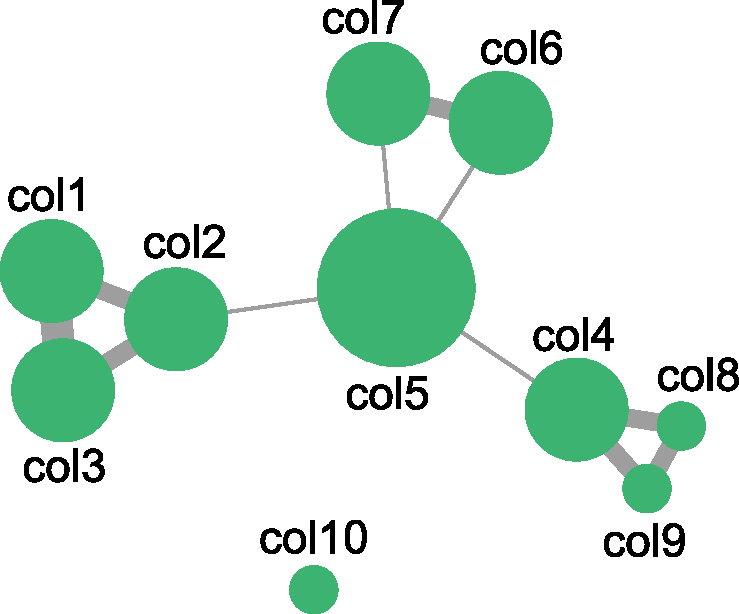
\includegraphics[width=.4\linewidth]{figures/network_models/cwn_generalaspect.pdf}
    \caption{General aspect of a Collectors Coworking Network (CWN). Coauthoring relationships between collectors (green nodes) are structured as edges in the graph, and are graphically represented as gray links.
    Here collectors nodes are sized according to the total number of records they've authored; and edges are weighted according to the number of collaborative records coauthored by both nodes.}
    \label{fig:cwn_general}
  \end{figure}

Differently from SCNs, where two entities classes are represented in the graph as disjoint nodes sets with the bipartite constraint, CWNs exclusively model direct relationships between entities from a single class (collectors), with the only connectivity restriction that a collector should not hold collaborative ties to itself.
The model is thus formally described as an unipartite (or one-mode) undirected graph
$$CWN = (S,E) \mbox{ ,}$$
where $S=\{u_1,u_2,...u_n\}$ is the graph's nodes set and $E$ is the set of undirected edges linking members of $S$.

Analogously to SCNs, both nodes and edges hold homonymous but conceptually distinct \textit{count} attributes.
Nodes count attribute stores the total number of records --- including non-collaborative ones --- a collector has authored, whereas
edges count attribute stores the total number of times an association between two collectors was observed in the dataset. Thus, although each node and edge respectively are uniquely included in $S$ and $E$, their recurrence patterns are registered in the model as attributes.
Another important edge attribute is the \textit{species list}. Although species associated to each occurrence record are not represented as entities in this model, edges can optionally keep a list of species that are shared by two collectors through that link, which is stored in this attribute.

Weights are assigned to edges in the CWN as a measure of their overall relevance in the network structure. Edges with higher weight values represent stronger collaborative ties between collectors, pointing out the main groups of collectors who are most willing to collaborate. 
The simplest rule is to set the edge weight as the total total number of occurrences of the tie it represents in the dataset. However, as pointed out by other authors studying social networks \cite{Newman2001a}, in reality not all collaboration acts should contribute the same way for a collector's network. 
Collectors tend to hold weaker collaborative ties with each other when they collaborate in larger teams than when they collaborate in smaller ones. 

The \textbf{hyperbolic weighting} rule accounts for this fact, while also considering the total number of collaborations between two collectors as a factor contributing the strength of their link.
According to this rule, not every new occurrence of the link increases the edge weight equally. 
The contribution of each new link depends on the number of the collectors $n^{(k)}$ included in record $k$ or, in other words, the team size. 
This rule follows a hyperbolic growth function 
\begin{equation}
w_{(i,j)} = \sum\limits_k \frac{\delta_i^{(k)} \delta_j^{(k)}}{(n^{(k)}-1)} \mbox{ , }
\end{equation}
where $\delta^{(k)}_u = 1$ if collector $u$ is in record $k$ and $0$ otherwise.
As the hyperbolic function above has singularity at $1$, it gets ill-defined for records with only one collector. 
Therefore only records with two or more collectors are used to compute edges weights. 
The maximum weight contribution of 1 is assigned to records with two collectors, whilst records with larger cliques yield smaller contributions.\\

Relationships in the CWN graph can be represented in a symmetric adjacency matrix $A^{n\times n}$ for which $a_{ij} \neq 0 \textit{ iff } (u_i,u_j) \in E$. 
Values of non-zero elements depend on the weighting method adopted for representing links strength, being the absolute counts of edges' recurrence (edges' \textit{count} attribute) the simplest one.
Additionally, the model's connectivity constraint states that all diagonal elements in $A$ are necessarily equal to $0$, thus ensuring that no self loops are formed.
To give a concrete example, the adjacency matrix for the graph in Figure \ref{fig:cwn_general} is 
$$
A =
\kbordermatrix{
& col1 & col2 & col3 & col4 & col5 & col6 & col7 & col8 & col9 & col10 \\
col1 & 0 & 2 & 2 & 0 & 1 & 0 & 0 & 0 & 0 & 0\\
col2 & 2 & 0 & 3 & 0 & 0 & 0 & 0 & 0 & 0 & 0\\
col3 & 2 & 3 & 0 & 0 & 0 & 0 & 0 & 0 & 0 & 0\\
col4 & 0 & 0 & 0 & 0 & 1 & 0 & 0 & 2 & 2 & 0\\
col5 & 1 & 0 & 0 & 1 & 0 & 1 & 1 & 0 & 0 & 0\\
col6 & 0 & 0 & 0 & 0 & 1 & 0 & 2 & 0 & 0 & 0\\
col7 & 0 & 0 & 0 & 0 & 1 & 2 & 0 & 0 & 0 & 0\\
col8 & 0 & 0 & 0 & 2 & 0 & 0 & 0 & 0 & 2 & 0\\
col9 & 0 & 0 & 0 & 2 & 0 & 0 & 0 & 2 & 0 & 0\\
col10 & 0 & 0 & 0 & 0 & 0 & 0 & 0 & 0 & 0 & 0
},
$$
where each element is the count of the total number of recurrences of collectors associations, represented in the graph as edges weights.




% Network construction
%% Singleton collectors are those holding no collaborative recording with any other collector in the dataset ($k=0$), and are also included in the model as isolated nodes.
\subsection{Model construction from data}

We build CWNs from species occurrence data in an iterative process that is similar to the one described for SCNs.
In this case, however, the only field that is strictly required for structuring relationships is the one containing collectors names, which in a database following \textit{Darwin core} terms standards should be named ``\textit{recordedBy}''.
The field containing species identities, although not required, can be optionally used during model construction in case the user decides to set the edges' \textit{species list} attribute.
Table \ref{table:cwn_example_dataset} shows the species occurrence dataset which was used to build the graph in Figure \ref{fig:cwn_general}.

\begin{table}[!ht]
  \caption{Species occurrence dataset from which the CWN model in Figure \ref{fig:cwn_general} was built. The \textit{species} field is not strictly required for building CWN models.}
  \begin{center}
  \begin{tabular}{r l c}
      id & recordedBy & species \\
      \hline
        0 & col1; col2; col3 & sp1\\ 
        1 & col3; col1; col2 & sp2\\ 
        2 & col1; col3 & sp3\\ 
        3 & col5; col4 & sp3\\ 
        4 & col5; col2 & sp3\\ 
        5 & col5; col6 & sp5\\ 
        6 & col5; col7 & sp4\\ 
        7 & col6; col7 & sp6\\ 
        8 & col6; col7 & sp7\\ 
        9 & col4; col8; col9 & sp4\\ 
        10 & col4; col9; col8 & sp5\\ 
        11 & col10 & sp6\\ 
        12 & col10 & sp6\\
       \hline
  \end{tabular}
  \end{center}
  \label{table:cwn_example_dataset}
\end{table}

For each row in the dataset, a \textit{clique} structure is formed by creating edges between all collectors included in the record's team, in a pairwise fashion. 
Each clique thus represents one collaborative act, where every collector gets and additional collaborative tie with every other collector included in that collaborative record. 
The clique size, which is the number of nodes included in the clique structure, is equivalent to the team size. For non-collaborative records the clique is composed by the collector node itself, and therefore no edges are formed.
As the user might want to distinguish the relevance of links originated from distinct team sizes, the hyperbolic weighting rule described in the previous section can be used for weighting links in each clique. 
In case the species field is included in the building routine, each clique also gets associated to the name of the species to which the recorded specimen belongs to.

The CWN model is finally composed by combining all cliques together into a single undirected graph. In this process edges that occur in multiple cliques have their weights summed. In case the species list attribute is set, combining edges also merges their respective species lists.




% Are unconnected collector represented in the model?
%% Average number of collaborators?


%% Weighting
%%% Check the weighting rule from Newman2001a -> Hyperbolic weighting

\chapter{Case Study: The University of Brasília Herbarium (UB) dataset}\label{casestudy_ub}
% herbarium page: http://florescer.unb.br/bol/
% Add herbarium historical

In this section I describe the application of the network models for deriving enriched information from the University of Brasilia Herbarium (UB) dataset.
The UB Herbarium is physically based at the University of Brasília Biology Department (UnB-IB) since its foundation in 1963.
The dataset is made publicly available for download through the Global Biodiversity Information Facility (GBIF) portal.
Here I assume the dataset has already been passed through a data cleaning process, and the entity resolution problem resolved.
Both CWN and SCN were built for supporting data enrichment.
Routines were written in Python3, using the Networkx and Pandas libraries.


Collectors had historical contributions to the herbarium \ref{table:ub_collectors_florescer}.

\begin{table}[H]
  \caption{Historically important collectors in the UB herbarium.}
  \begin{center}
  \begin{tabular}{l c c}
      & activity years & contribution\\
      \hline
      William R. Anderson & 1962-1976 & Central Brazil Expedition (NY Botanical Garden)\\
      Howard S. Irwin & 1962-1976 & Central Brazil Expedition (NY Botanical Garden)\\
      George Eiten & - & Cerrado biome, mainly in MA state \\
      James Alexander Ratter & 
      	\begin{tabular}[t]{{@{}c@{}}}1968-1976 \\ 1996-2006\end{tabular} &
        \begin{tabular}[t]{{@{}c@{}}}Xavantina-Cachimbo expedition \\ Cerrado biome\end{tabular} \\
      Joseph Harold Kirkbride Junior & 1976-1983 & Flora of DF \\
      Ana Lúcia Tostes Leite & 1982-1984 & Continental algae of DF \\
      Carolyn Elinores Barnes Proença & 1981-current & Cerrado biome \\
      Maria das Graças Machado de Souza & 1982-current & Continental algae of DF and GO\\
      \hline
  \end{tabular}
  \\[1.5em]
  \hfill Source: FLORESCER Project webpage \cite{florescer}
  \end{center}
  \label{table:ub_collectors_florescer}
\end{table}

\subsection{Dataset Characterization}

%%%%%%%%%%%%%%%%%%%%%%%%%%%%%
%% Taxonomic characterization

After loading the dataset with specified columns into memory I've filtered out records with missing values for fields \textit{recordedBy} or \textit{scientificName}, as these are critical for building the network models.
At the time of this study the resulting dataset had a total of 185301 records. However not all records have been identified up to the taxonomic resolution of \textit{species}, as shown in Table \ref{table:dset_taxonomicres_counts}. 
As taxons hold a tree-like hierarchical relationship, those at more inclusive (broader) ranks can be successfully derived from more restrictive ones, but not the inverse. Each child taxon have exactly one parent, but a parent taxon can have one or more children.
To give an example, the table shows that approximately $76\%$ of the records are at the resolution of species. However the species identity of records at higher resolutions, in this case form or variety, are automatically determined by following parental paths. This makes species identity derivable for approximately $82\%$ of the records, as shown in the cumulative percentage for the species rank.

For the construction of SCNs we must make sure only to include records that were identified up to the same taxonomic resolution as the model itself, keeping in mind that lower-resolution entities can be derived from higher-resolution ones. 
For CWNs, on the other hand, the taxonomic resolution of each record is not relevant for model construction, as edges are built using only collector cliques. In this case all records with at least two collectors can be used, irrespective of their taxonomic resolution.

\begin{table}[H]
  \caption{Number of records with maximum taxonomic resolution at each rank. Ranks are ordered hierarchically, being \textit{FORM} the most restrictive (higher resolution) and \textit{KINGDOM} the broader (lower resolution) one. Cumulative metrics show the total amount of records that could be derived for each rank.}
  \begin{center}
  \begin{tabular}{l c c c c}
       & count & \% & cumulative count & cumulative \% \\
      \hline
      FORM & 1000 & 0.5397 & 1000 & 0.5397\\
      VARIETY & 8935 & 4.8219 & 9935 & 5.3615\\
      SUBSPECIES & 1681 & 0.9072 & 11616 & 6.2687\\
      SPECIES & 140763 & 75.9645 & 152379 & 82.2332\\
      GENUS & 24397 & 13.1661 & 176776 & 95.3994\\
      FAMILY & 6223 & 3.3583 & 182999 & 98.7577\\
      PHYLUM & 294 & 0.1587 & 183293 & 98.9164\\
      KINGDOM & 2008 & 1.0836 & 185301 & 100\\
      \hline
      total & 185301 & 100 & &
  \end{tabular}
  \end{center}
  \label{table:dset_taxonomicres_counts}
\end{table}

% what are the main families?

\begin{table}[H]
  \caption{Number of distinct taxons at each taxonomic rank in the dataset. For each rank a list with its top-5 most recorded taxons is included with their respective counts.}
  \begin{center}
  \begin{tabular}{l c c c}
   & num of taxons & top-5 taxons & num of records \\
   \hline
    kingdom & 5 &
	\begin{tabular}[t]{{@{}c@{}}}Plantae\\Chromista\\Fungi\\Bacteria\end{tabular} &
	\begin{tabular}[t]{{@{}r@{}}}179218\\4204\\1391\\342\end{tabular} \\ \\
    phylum & 12 &
	\begin{tabular}[t]{{@{}c@{}}}Tracheophyta\\Bryophyta\\Ochrophyta\\Charophyta\end{tabular} &
	\begin{tabular}[t]{{@{}r@{}}}153589\\16485\\4133\\3500\end{tabular} \\ \\
    class & 29 &
	\begin{tabular}[t]{{@{}c@{}}}Magnoliopsida\\Liliopsida\\Bryopsida\\Bacillariophyceae\end{tabular} &
	\begin{tabular}[t]{{@{}r@{}}}126288\\23004\\15899\\4133\end{tabular} \\ \\
    order & 136 &
	\begin{tabular}[t]{{@{}c@{}}}Myrtales\\Fabales\\Poales\\Malpighiales\end{tabular} &
	\begin{tabular}[t]{{@{}r@{}}}24312\\20846\\17159\\16188\end{tabular} \\ \\
    family & 507 &
	\begin{tabular}[t]{{@{}c@{}}}Fabaceae\\Myrtaceae\\Asteraceae\\Rubiaceae\end{tabular} &
	\begin{tabular}[t]{{@{}r@{}}}19254\\12833\\11271\\9447\end{tabular} \\ \\
    genus & 3374 &
	\begin{tabular}[t]{{@{}c@{}}}Myrcia\\Eugenia\\Mimosa\\Miconia\end{tabular} &
	\begin{tabular}[t]{{@{}r@{}}}4654\\3750\\2992\\2402\end{tabular} \\ \\
    species & 15379 &
	\begin{tabular}[t]{{@{}c@{}}}\textit{Myrcia splendens}\\\textit{Myrcia guianensis}\\\textit{Eugenia punicifolia}\\\textit{Sematophyllum subpinnatum}\end{tabular} &
	\begin{tabular}[t]{{@{}r@{}}}696\\560\\462\\438\end{tabular} \\
  \hline
  \end{tabular}
  \end{center}
  \label{table:taxons}
\end{table}

%%%%%%%%%%%%%%%%%%%%%%%%%%%%%%
%% Geographic characterization

From the set of $185301$ records approximately $48\%$ (a total of $89216$) were interpreted and tagged as having geospatial issues during internal preprocessing routines in the \textit{GBIF} platform \cite{GBIF.ORG}.
During geospatial validation the routines check for each record ($i$) if geographical coordinates are erroneously assigned to zero latitude and longitude; ($ii$) if geographic coordinates are in fact placed within the boundaries of the country if indicated; and ($iii$) if lat/long values are likely to having been swapped or negated during recording.
If inconsistencies are detected during the execution of such routines, issues are registered for each record, priorly to making the dataset available for download or query via API. 
% http://www-old.gbif.org/infrastructure/processing

As shown in Figure \ref{fig:venn_geospatial_issues} most geospatial issues are due to records being assigned to zero coordinates (zero latitude and longitude), which also makes them laying outside of the country boundaries. As a consequence they are tagged as having both the ``Zero Coordinates'' (ZC) and ``Country Coordinates Mismatch'' (CCM) issues, being represented in the figure as the intersection between CCM and ZC.
Some records with only the CCM issue were not misplaced in coordinates $(0,0)$, but still were improperly placed outside the country frontiers. 
On the other hand, records with only the ZC issue are those which were misplaced in coordinates $(0,0)$ but were lacking information about the country, and therefore couldn't be classified as being outside the country frontiers.

  \begin{figure}[h!]
  	\centering
    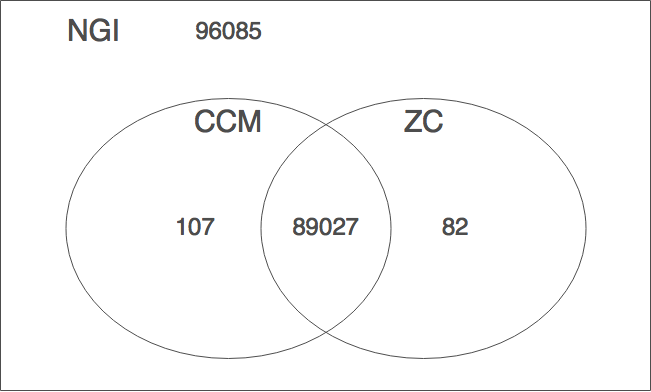
\includegraphics[width=0.6\linewidth]{figures/venn_geospatial_issues.png}
    \caption{Number of occurrences from the UB herbarium dataset classified within each geospatial issue class. \textit{NGI}: Records with no geospatial issues; \textit{CCM}: Country Coordinates Mismatch issue; \textit{ZC}: Zero Coordinates issue.}
    \label{fig:venn_geospatial_issues}
  \end{figure}

Records without geospatial issues comprise approximately $52\%$ of the dataset, and their coordinates are shown in Figure \ref{fig:occurrence_map}. Notice that the figure extent is constrained around the Brazilian territory, and records outside the canvas are omitted. Although most records deposited in the UB herbarium were collected in Brazil, there is also a considerable amount of records from many other countries (Figure \ref{fig:recs_by_cntry_state}(a)), that were been obtained from herbaria exchange activities or international recording expeditions. According to the herbarium description available from the \textit{Florescer project} webpage \cite{florescer}, records from the Amazon and Atlantic forest were mostly exchanges under the curatorship of \textit{Dr. João Murça Pires} and \textit{Dr. Graziela Maciel Barroso}, respectively. A considerable part of international records were exchanges incorporated under the curatorship of \textit{Dr. George Eiten}.  


  \begin{figure}[h!]
  	\centering
    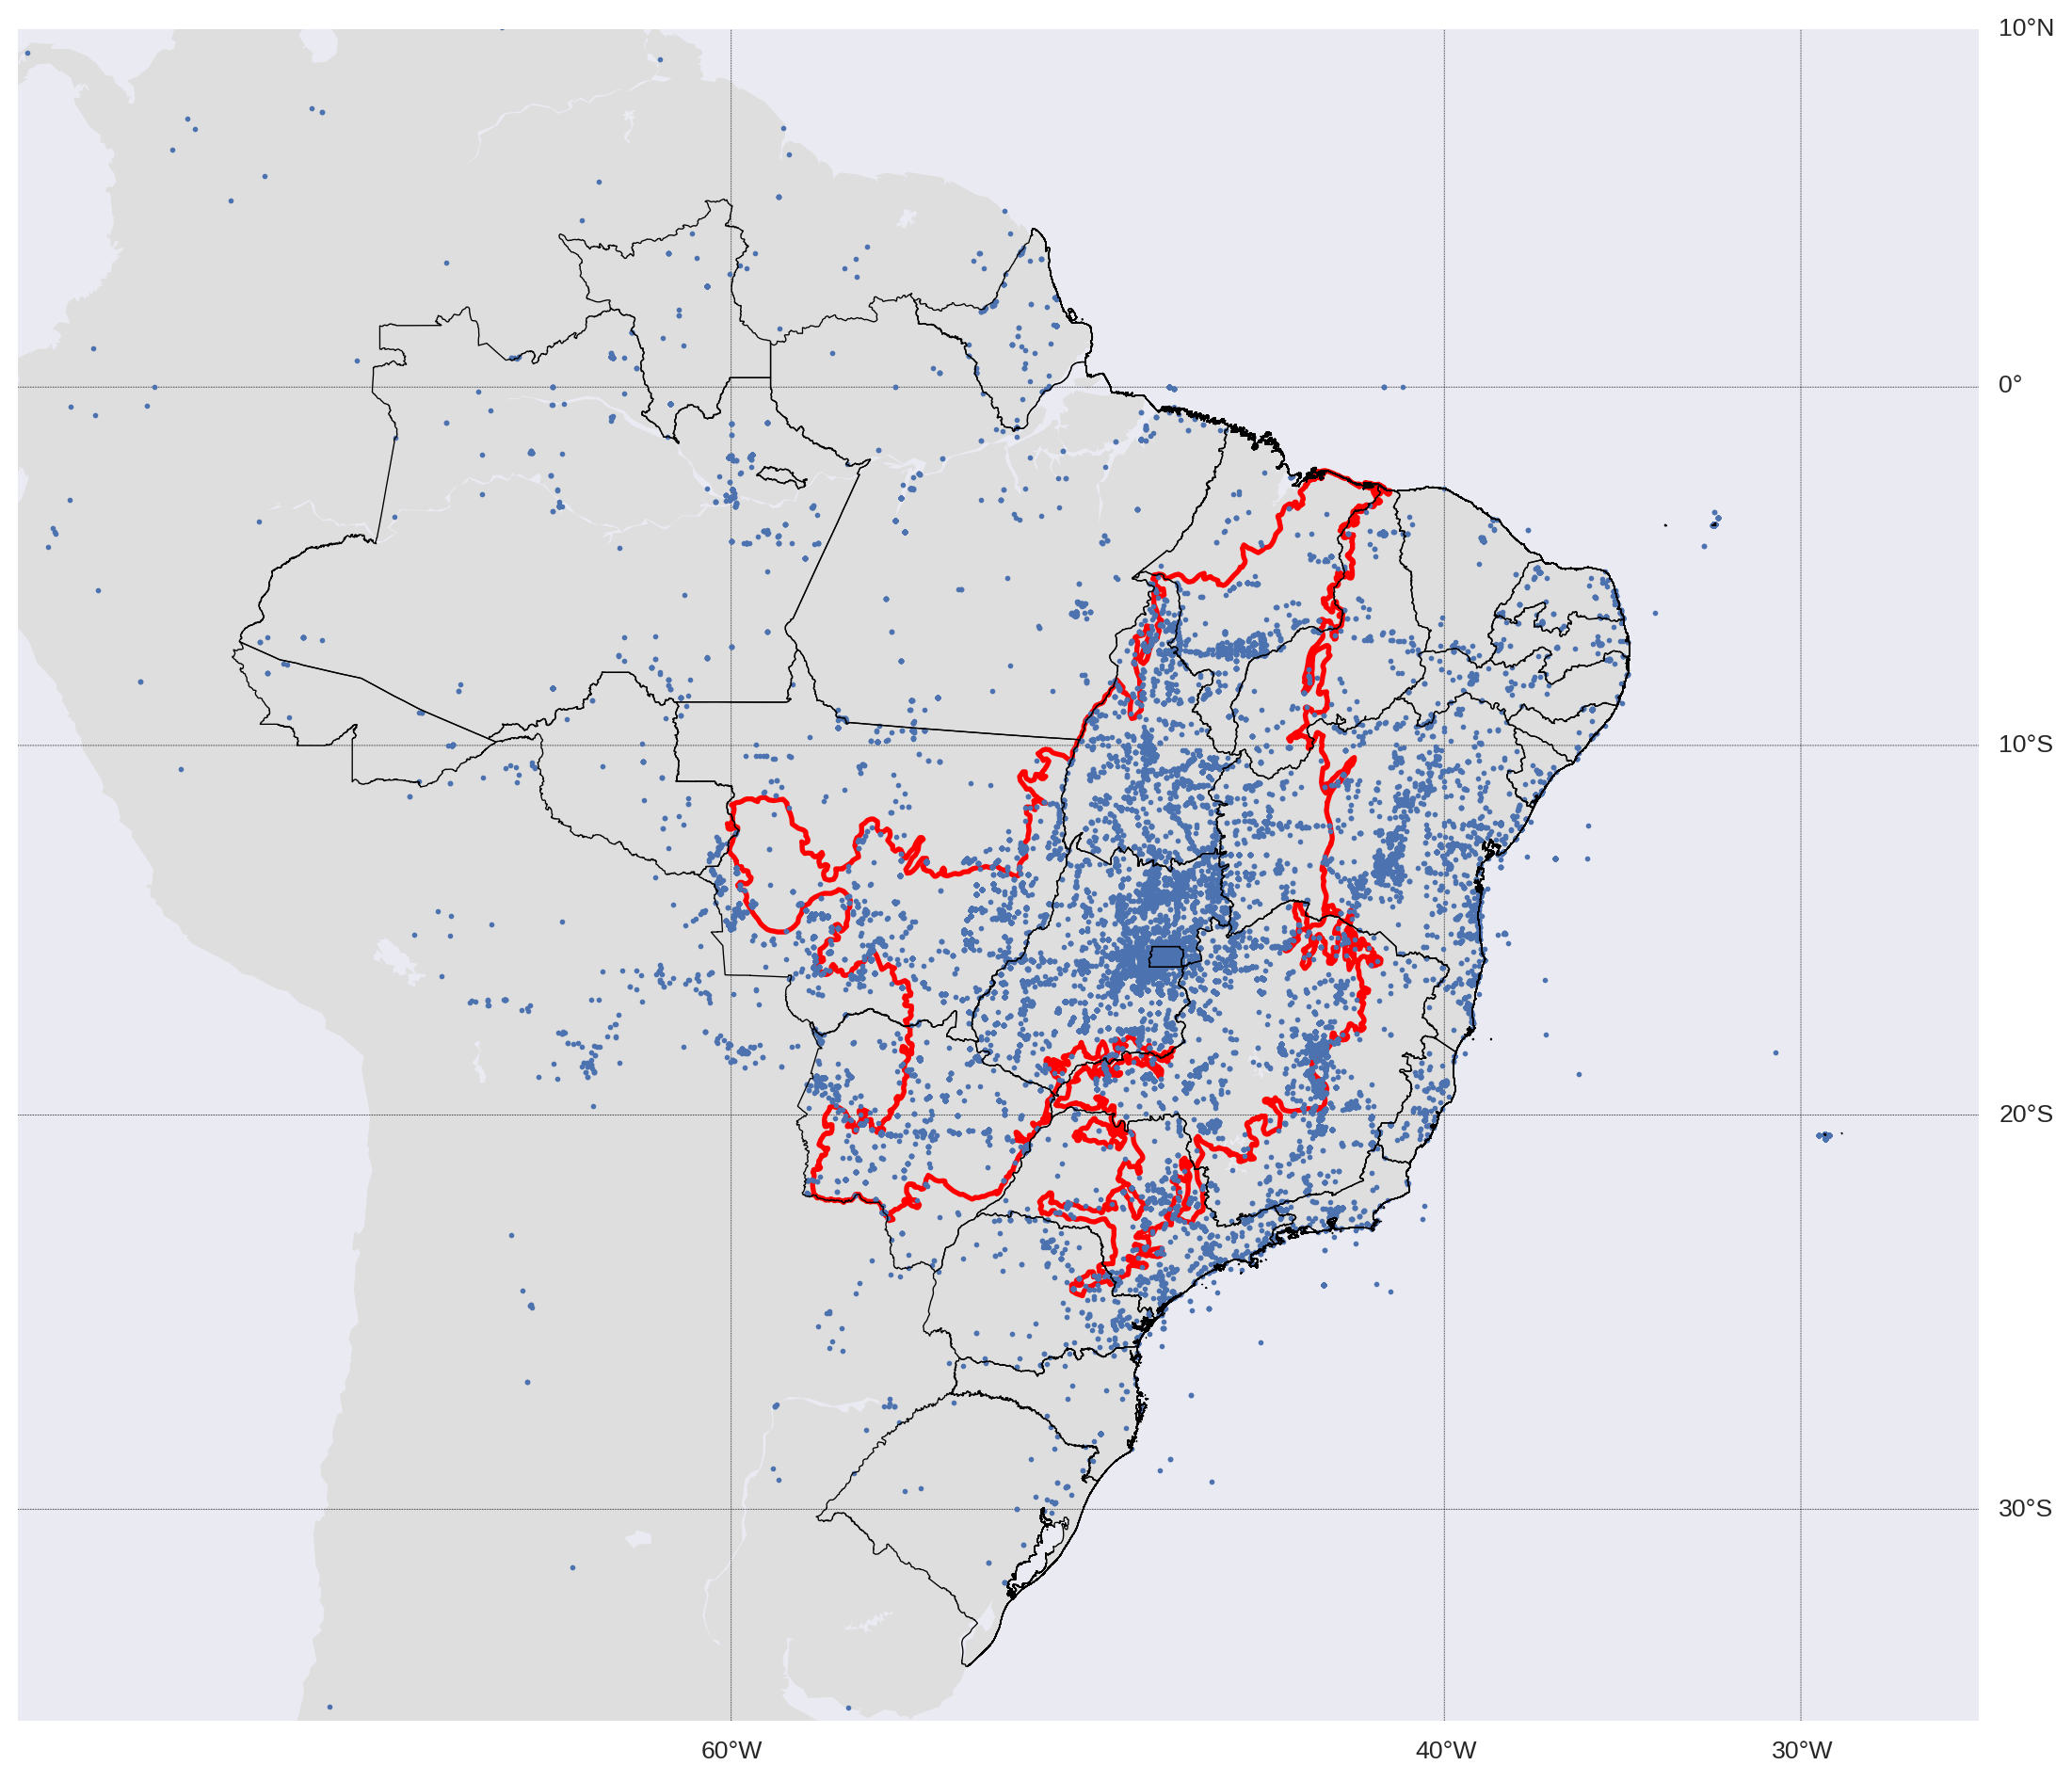
\includegraphics[width=0.7\linewidth]{figures/occurrence_map.png}
    \caption{Geographic distribution of the occurrences from the UB Herbarium dataset near the Brazilian territory. Records without geospatial issues are placed in the map as blue dots. The area outlined in red represents the boundaries of the Cerrado biome.}
    \label{fig:occurrence_map}
  \end{figure}
  
Within the Brazilian territory, the Federal District was the most sampled federative unit despite its small area, followed by the state of Goiás (\ref{fig:recs_by_cntry_state}(b)). 
Such a geographic bias in the occurrences distribution can be explained by the fact that UB is physically located in the University of Brasilia, making it more viable for associated collectors to record in nearby locations.
Moreover, as UB is a national reference herbarium for species occurring the Cerrado biome, botanists working in Cerrado areas become more inclined to deposit their recordings in the institution.
In fact, figure \ref{fig:occurrence_map} shows that UB records are more densely concentrated within the Cerrado biome, mostly in the Central Brazil region. 

  \begin{figure}[h!]
  	\centering
    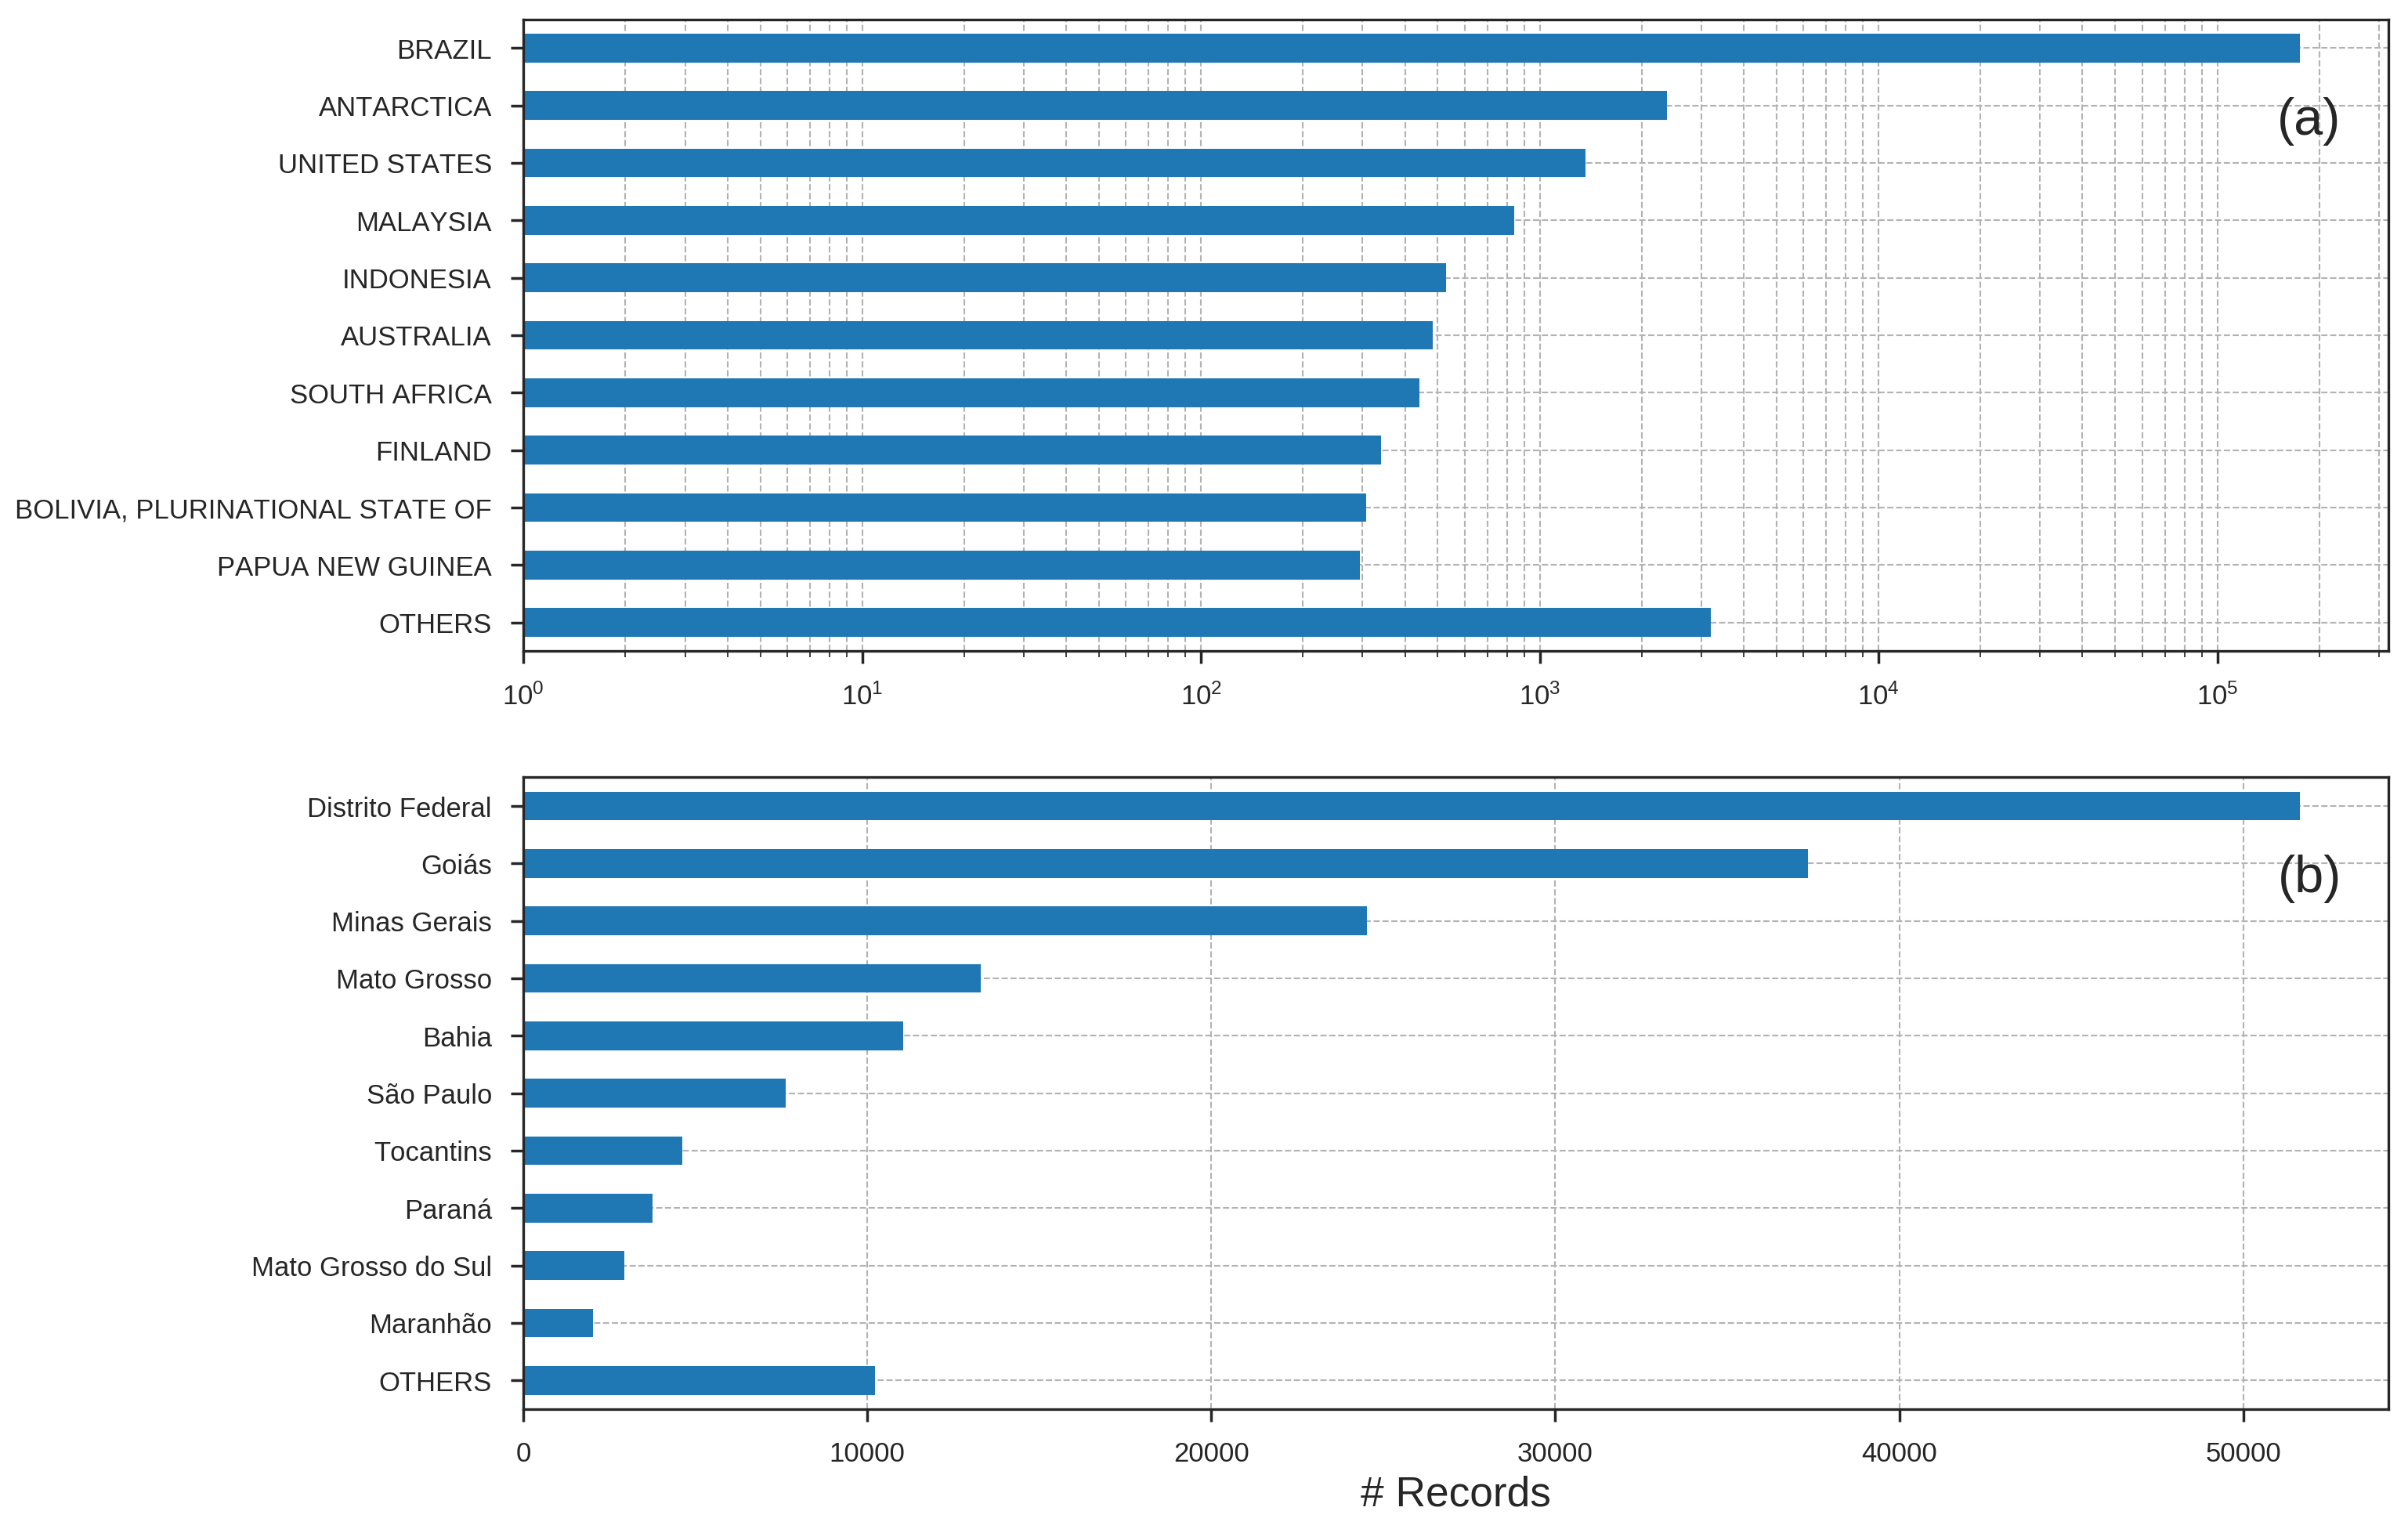
\includegraphics[width=\linewidth]{figures/recs_by_cntry_state.png}
    \caption{Top-10 countries (a) and top-10 Brazilian states (b) with most occurrence records deposited in the UB herbarium. Records from countries and states beyond the $10th$ position in the respective ranks are summed and assigned to \textit{OTHERS}.}
    \label{fig:recs_by_cntry_state}
  \end{figure}
  
%%%%%%%%%%%%%%%%%%%%%%%%%%%%
%% Temporal characterization
Almost $98\%$ of the records contain information about their collection dates.
The oldest records in the herbarium dataset date from 1800.
However, more intensive collection activity started around 1960. Around 8000 records in the herbarium date up to that time (Figure \ref{fig:ub_records_timeseries}(c)). %reference cumulative-log figure
From 1950 to present, there are two apparent peaks in collection activity around year 1965 and 2013 (Figure \ref{fig:ub_records_timeseries}(a)). % Why?

  \begin{figure}[h!]
  	\centering
    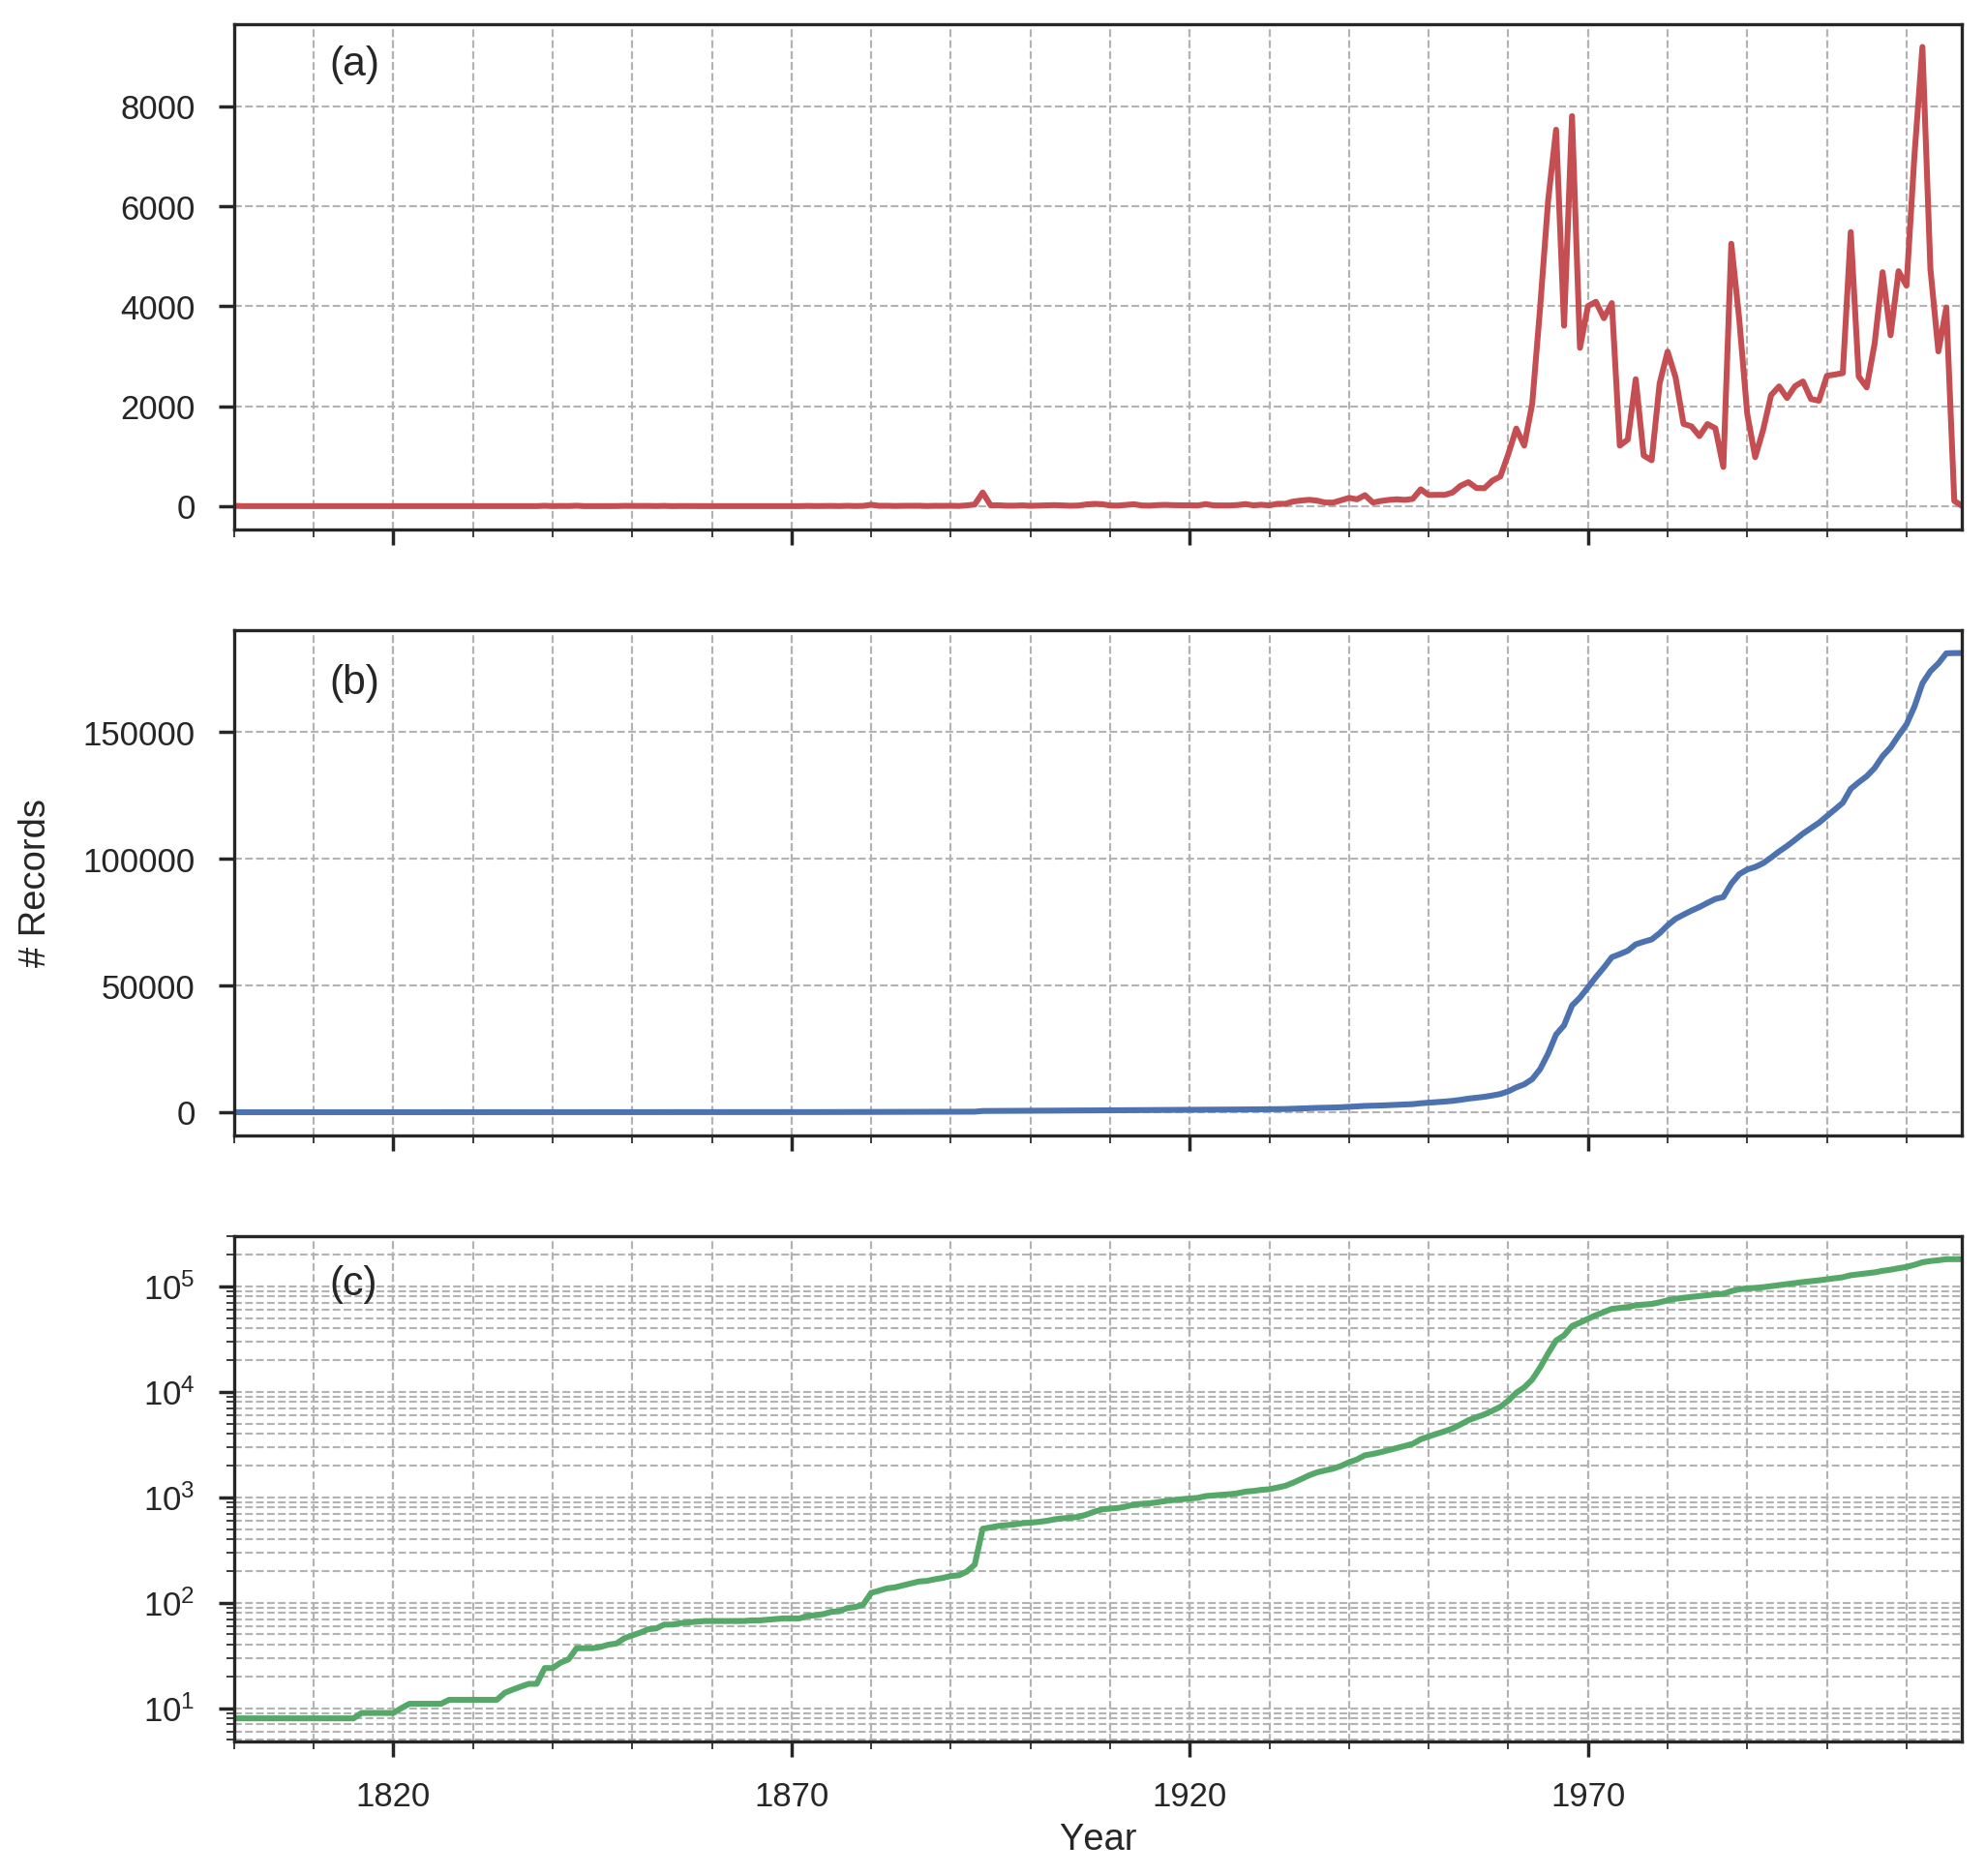
\includegraphics[width=\linewidth]{figures/ub_records_timeseries.png}
    \caption{Recording activities registered in the UB herbarium since 1800, aggregated by year. (a) Absolute record counts for each year. (b) Cumulative counts of records in a linear scale. (c) Cumulative counts of records using a logarithmic scale.}
    \label{fig:ub_records_timeseries}
  \end{figure}


\subsection{Network models construction}
%%%%%%%%%%%%%%%%%%%%%%%%%%%%%%
%%%%%%%%%%%%%%%%%%%%%%%%%%%%%%
%% Network models construction


% Build SCN
% What is the species with more collectors? What is the collector with more species?
% Average collector/species & species/collector  (with percentages)

% Projections

% Similarity between collectors
% It should be noticed, however, that in practice collectors holding similarity values very close to one tend to be those with very few records in the dataset. More experienced collectors can have higher similarities with some collectors, but it is usually not very high.
%% PLOT max similarity vs degree


%%% QUESTIONS

%% 1. How common are collaborative recordings within the dataset?
%%% What is the proportion of collaborative records in the dataset? How many collaborators
%%% One-collector recording vs >2 collectors recordings
%%% Distribution of team size
%%% Caveats: Some collectors may not include collaborators names in the records

%% x. How likely is a novice collector to become a great collector?

%% x. Do collectors with similar interests tend to collect together?
%%% Mix of the two models
%%% Look for homophily in collectors communities, assortativity.

%% x. Which groups of species best modularize collectors in the dataset, in terms of their collection interests? 
%%% Using SCNs
%%% Are these groups necessarily taxonomic ones (such as family)? Or could functional groups be more relevant in some cases? Or is there a geographical effect?
%%% e.g. Some group might be best classified as specialists on species inhabiting some geographical location, with some specific habit and belonging to some family rather than simply as specialists in a given family.

%% x. The Expert-location problem {Chapt. 8 of book Social Network Data Analytics}
%%% The expert team formation problem: How can we best select experts for a given job, based on how willing they are of collaborating together?
%%% Combine both SCN and CWN
\newcounter{QuestionsCounter}
\setcounter{QuestionsCounter}{1}

\subsubsection*{Question \arabic{QuestionsCounter}: How prevalent are collaborative records?}
blablabla2

\subsubsection*{Question \arabic{QuestionsCounter}: <Another question>}


% References {Newman2004}
% Statistical characterization of SCN structure
%% Species per collectors (species bag), collectors have species signatures
%% Collectors per species
%% Simply projecting this graph originates a very densely-connected network, failing to reveal relevant connectivity patterns (Lambiotte2005)

%% Define finer species taxonomic/functional division that best reflect collectors interests than division by family alone (Lambiotte2005)
%%% Do collectors interests communities reflect taxonomic divisions such as the family level?


% Statistical characterization of CWN structure
%% Largest component, connected components...
%% Assortativity: Do collectors with many collaborators (very collaborative) tend to associate with others that are also very collaborative?

% Network Evolution
%% Is network evolution ruled by preferential attachment?
%% How likely is it that two co-authors of a record will also be co-authors of another one?
%% Do attach influential collectors (high betweeness) attach preferentially to other influential ones? (Goh2003, Newman2004)


\subsection{Degree distribution?}

A first step for characterizing the network is to obtain its degree distribution.
The degree distribution was obtained for both 


\subsection{Who are the most central collectors in this herbarium?}





\subsection{Features Selection}

%% Features engineering



\section{Model Evaluation}



\chapter{Conclusion and Perspectives}\label{conclusion_perspectives}
% ===========
% Conclusions
% -----------
In this dissertation, we proposed the conceptual basis of a new approach for describing the assemblage of biological collections as a social process, driven by the taxonomic interests of contributor collectors as well as their social interactions.
In this context, we provided methods for structuring species occurrence data from biological collections into two main classes of network models, each giving distinct perspectives on the recording behavior of collectors.
\textbf{Species-Collector Networks} (SCNs) model interest relations between collectors and taxa they record, whilst \textbf{Collector CoWorking Networks} (CWNs) represent collaborative ties between collectors co-authoring records of specimens. 
% UB case study
As a case study, we demonstrated the use of our network models by exploring the species occurrence dataset of the University of Brasília Herbarium~(UB).
Using the social network analytics framework \cite{Barbier2011,Stork2015} as a theoretical foundation, we explored structural properties of the studied networks as well as 
investigated the formation of communities of collaboration and common interests.
We also assessed the distinctiveness of collectors regarding their taxonomic interests, their collaborativity with others, and the temporal evolution of collaborative recording in the herbarium.
Although in this study we specifically discuss SCNs and CWNs in the context of scientific biological collections, the same ideas here exposed can be also extended to other communities, such as those of nature observers (\textit{e.g.} wildlife photographers, bird watchers) and citizen scientists.
% TODO: check uniformity of using italics in e.g., i.e. and itemized lists.

% Why structure collections data as networks?
We believe our network models provide the structural basis for a more realistic understanding on how collector and taxonomic biases arise in biological collections. 
As stated by \citeonline{Marin2011}, network-based approaches allow analysts 
(\textit{i})~to investigate the effects of interactions between individuals on shaping their own behaviors, rather than simply comparing static attributes of individuals within a population; and
(\textit{ii})~to investigate the formation of non-homogeneous communities, composed of individuals interacting with their groups at varying levels of commitment.
We consider that these two aspects are particularly relevant in the context of biological collections.

First, collectors often start their careers being supervised by one or more experienced collectors.
As it naturally happens in many social systems, the behavior of individuals can be strongly influenced by others at more privileged positions, and this is likely to be the case for collector communities as well.
A network-based approach would allow us to investigate, for instance, how the collecting behavior and taxonomic interests of novice collectors are shaped by their association with more experienced ones.
Moreover, depending on its position on the network, a collector can interact with multiple groups of collectors at different extents, thus assuming the role of influencer in some cases while being influenced in others.
The influential power of a collector depends not only on the absolute number of connections it holds with others, but also on how strongly it intermediates other connections, how close it is to every other collector in the network, and how influential are its own connections. % Influential analysis
All these aspects can be assessed using well-known network centrality metrics (including degree, betweenness, closeness, and eigenvector centralities), and could be used for investigating which collectors are the most relevant for shaping the taxonomic composition of a biological collection. 

Second, although collectors often define their own taxonomic interests and expertises in terms of natural or functional groups of organisms, those are not necessarily the groups that best split the interests of collectors in the dataset of a given collection.
In addition, collectors~(even the most specialized ones) are not restricted towards exclusively recording organisms of their expertises, nor they have uniform interest towards all of those organisms.
%
In this context, SCNs provide the structure for discovering groupings of taxa that are better for characterizing and differentiating collectors based on their taxonomic interests~(communities in the species projection); and for investigating associations of collectors with groups of taxa in a non-discrete manner, allowing collectors to be linked to taxa at multiple groups and at different intensities.
%
In fact, while some groups of taxa are more specifically recorded by distinctive communities of specialized collectors, others are recorded by a wider range of collectors, with diverse taxonomic interests.
For instance, the SCN of the UB herbarium suggests that collectors specialized in families \textit{Myrtaceae}, \textit{Poaceae}, or \textit{Piperaceae} form communities of interests which are in fact more distinctive, as those families are relatively poorly recorded by collectors who are not specialists in each of them (see Figure \ref{fig:ub_scn_family_projSp_communities}).
In contrast, other families, such as \textit{Fabaceae}, \textit{Melastomataceae}, and \textit{Rubiaceae}, are more widely recorded in the herbarium, thereby they do not form a tight community of interest.

% Quality of the model
The quality of our network models strongly depends on the quality of the species occurrence dataset that is used to build them, more specifically on the fields containing the names of the collectors (\textit{recordedBy}, in TDWG standards) and the taxonomic identity of the specimen (\textit{scientificName}, in TDWG standards) of each record.
%
During this study, we have explored occurrence datasets from other herbaria other than the UB, including the RB~(at the Rio de Janeiro Botanical Garden) \cite{gbif_rb}, 
the MBML (Mello Leitão Herbarium) \cite{gbif_mbml},
and the Hemilio Goeldi Museum Herbarium \cite{gbif_mpegh}.
Nevertheless, we decided to only use the dataset from the UB in our case study because of its relatively high quality, specifically for the two aforementioned fields.
%
In all other herbaria, the collectors field (\textit{recordedBy}) was particularly problematic.
Our hypothesis is that the low quality of this field is associated with its low value for most uses of species occurrence data, implying that not much effort has been employed by data curators towards improving the data quality of this field.
While imprecise taxonomic determinations in the \textit{scientificName} field would also lead to low quality networks, this field is critical for many other applications of occurrence data, and thus improving its quality has been extensively pursued by the biodiversity informatics community.
The most common and impacting issues associated with the collectors field were: 
($i$)~using inconsistent delimiter characters for separating the names of each collector in a record, leading to many non-atomized names and consequently to the existence of nodes in the network that represent more than one collector; 
($ii$)~registering collectors names using inconsistent naming conventions, which makes it hard to systematically interpret what are the component parts of a name; 
($iii$)~using multiple name variations for a collector, leading to collectors being represented by more than one node in the resulting network; and 
($iv$)~only including the name of the first collector in records (and eventually aggregating all secondary collectors under the expression `\textit{et al.}'), which is interpreted as an absence of collaborative ties and thus does not contribute for the formation of edges in CWNs.
Constructing the network models from a low-quality dataset can therefore introduce several semantic imprecisions. 
% RecordedBy: Two classes of issues: (1) Naming inconsistencies; (2) Authorship omission

% Limitations of the model
Our network models, as proposed in this dissertation, also have a set of limitations, which should be addressed in the future.
% The networks only reflect the view of a single institution -> joining multiple herbaria datasets
First, as the networks are built in a single step using a single dataset (which is usually provided by a single institution), they only represent a partial view of the real interests and collaborations that collectors have accumulated during their careers.
For obtaining a more holistic representations, a mechanism for dynamically joining multiple occurrence datasets---and eventually other types of data---should be incorporated to the models.
Although one might argue that multiple datasets can be simply merged before they are passed to the constructors of the models, that would still consist of a one-step construction, requiring the availability of all data at the first place.
In addition, if any other dataset were to be incorporated in the future, the model would need to be entirely reconstructed, and all necessary preprocessing routines would have to be re-executed in each one of the previous datasets.
%
We believe that the most challenging aspect of joining multiple datasets would be addressing the entity resolution problem across different datasets from multiple sources. A possible solution would be to map entities in each dataset to unique identifiers (such as those from the ORCID\footnote{\url{https://orcid.org/}} initiative or the id in the Lattes platform,\footnote{\url{http://lattes.cnpq.br/}} the latter widely adopted by the Brazilian scientific community) using a crowdsourcing strategy, described later in this chapter.

% The geographic and temporal dimensions
Another important limitation of our network models is that they are static and non-spatialized~(\textit{i.e.}, they are temporally and geographically invariant), and limited to representing relationships of a single type each. This implies that relationships modeled in both networks are assumed to occur irrespective of temporal and geographic dimensions, which is clearly limiting for the phenomena they model.
As the careers of collectors have limited lifespans, they can only possibly collaborate with others if their activity periods overlap in time.
In addition, both coworking~(between collectors) and interest~(involving a collector and a taxon) relationships derive from collecting events---each happening at a determined geographic location and at some point in time---, being thus temporally and spatially constrained.
Incorporating these two dimensions to our models is also central for capturing network evolution in their structure.
%
As in many other social systems, relationships in SCNs and CWNs change in time, as new ties are constantly formed while older ones are broken.
It is reasonable to consider that collectors interact with distinct groups of people throughout their careers, assuming distinct roles in each relationship.
For instance, we hypothesize that earlier in their careers, collectors are more likely to assume relationships and have their interests influenced by their academic supervisors or other collectors who are more experienced.
On the other hand, relationships assumed by collectors later in their careers tend to be the opposite, as they assume the role of the more experienced collector~(and thus, the influencer).
Further, depending on the stage of a collector's career and the groups of collectors he/she interacts at that moment, we might observe substantial shifts in his/her taxonomic interests (while changes in his/her taxonomic interests can also lead to collaborating with different groups).
Other factors can also influence the patterns of recording activity of a collector, including oscillations in the availability of financial resources for field expeditions, and changes in his/her residence location.
% A diversity of representations for temporal networks have been proposed, which can be categorized as either lossless representations, or lossy representations \cite{Holme2015}.

% Adopting an unifying structure
% SCNs and CWNs should be stored in an unified structure, for example using the structure of multiaspect graphs (MAGs).
% MAGs allow representing edges composed of multiple features by using general graph theory, instead of tensor algebra.
% Important dimensions can be included as aspects, such as temporal and spatial, and different types of edges. 
As many applications using our network models would need to combine the perspectives of both SCNs and CWNs, we also recognize the importance of adopting an unifying model for seamlessly integrating the two networks into a single structure.
The requirement for such a model is that it represents two types of connections (interest and coworking) and two distinct sets of nodes (collectors and species), besides incorporating the temporal and geographical dimensions into its structure.
Although the concept of \textit{multilayer networks} provides a solution for modeling dynamic complex systems with many aspects of connectivity, literature around this topic is still incipient, with many proposals though little consensus on the best way to represent them~\cite{Kivela2014}.
In this context, \citeonline{Wehmuth2014} have introduced the concept of \textit{Multiaspect Graphs} (MAGs) as a graph extended abstraction for high order networks that operates on a structure that is proved to be isomorphic to traditional directed graphs.
By using the structure of a MAG, the set of vertices, layers, time instants, and geographic locations can be then represented as 4 distinct \textit{aspects}; and edges as $8$-tuples, composed of pairs of elements of each aspect.
Moreover, key properties and algorithms that have been widely used for analyzing directed graphs are also extended to MAGs, which makes them a relatively simple representation for higher-order graphs \cite{Wehmuth2015}.

Finally, for a direction towards further developments of this work, we indicate the incorporation of geographic and temporal dimensions to the networks as top priorities.
We also conclude our text by briefly presenting some possible new perspectives of ideas for applications (some of them still very rough) that could potentially make use of our network models. 
Many examples below assume that temporal and geographic dimensions are already included.

% ============
% Applications
% ------------
\newcounter{ApplicationCase}

% Collectors Profiling and activities history
% -------------------------------------------
% Profiling collectors in terms of their activities and interests can be a way of further detecting anomalies (activity monitoring, Fawcett and Provost 1999).
% Collectors temporal, geographic and taxonomic ranges \cite{}.
% The study of collectors career trajectories cite{Borgatti2015 conclusion}.
\stepcounter{ApplicationCase}
\paragraph*{\theApplicationCase. Profiling collectors.}
An important improvement towards a systematic understanding of the roles, interests, and behaviors of collectors in a biological collection is grouping them into discrete profiles.
Profiles aggregate semantic value to the model, as they allow domain analysts to summarize the complex variety of collector features into general classes that are more comprehensible to them.
%
For instance, analysts may be interested on inferring \textit{academic roles} of collectors (\textit{e.g.} professor, student, or field assistant), whether collectors are currently \textit{active} or \textit{retired}, or still whether they are \textit{experienced} or \textit{novice}.
Similarly, collectors can be classified as \textit{innovators} if they collect taxonomic groups that have never been recorded by others in the collection, or \textit{followers} if they follow the interests of others;
as \textit{visitors} if they contribute to the collection in bursty patterns, or \textit{residents} if they contribute to it a regular basis;
\textit{specialists} or \textit{generalists}, regarding how specific their taxonomic interests are;
\textit{regionalists} or \textit{travelers}, regarding their interests to collect at many distinct localities.
Compositions of each of these aspects, which we refer to as \textit{characteristics} of collectors, are used to define \textit{collector profiles}.
Considering that the interests and collecting behavior of collectors change in time as they get more experienced, profiles are naturally dynamic.
A simplistic approach for representing such variations would be to associate profile timelines with collectors, composed of multiple discrete events documenting profile changes.
%
Profiling collectors can be generalized to a network problem known as the \textbf{node classification problem}~\cite{Bhagat2011}.
Starting from a subset of nodes that are previously labeled (profiled), the goal is to train a machine learning classifier that learns which compositions of features lead to each profile.
Next, in an iterative process, non-profiled nodes have their profiles predicted based on their attributes.
Network structure can be useful in this process, as it allows the propagation of labels (profiles) among collectors, using their positional features and patterns of association.


\stepcounter{ApplicationCase}
\paragraph*{\theApplicationCase. Contextual enrichment of occurrences.}
One of the main complexities of characterizing bias in occurrence records is that they are typically obtained in an opportunistic way, without the adoption of systematic sampling designs.
Specimens are also collected in a high variety of contexts, from \textit{botany field classes} mainly composed of naive students to \textit{big survey projects}, involving many teams of expert collectors.
Surveys can also be characterized as being \textit{focal}, if individuals from a specific taxonomic group are thoroughly searched; or \textit{generalist}, if the goal is to document the diversity of organisms at a location as comprehensively as possible.
Also some records may result from a \textit{herbarium exchange}.
Considering that different contexts lead collectors to behave and collaborate differently during collection activities, enriching occurrence records with contextual information could make them more comparable, potentially helping to characterize biases and sampling efforts. 
%
One idea worth investigating is whether the composition of collectors associated with a record convey contextual information about it.
For instance, observing groups composed of many novice collectors associated with one or two who are very experienced, recording in areas relatively well explored by others, could indicate that those records have been obtained in the context of a field course.
Records in which all collectors are substantially experienced but with distinct interests, on the other hand, could indicate the context of exploratory surveys.
%
Moreover, additional attributes of the recorded species can also be inferred from the composition of collectors.
For instance, \citeonline{TerSteege2011} observed that experienced collectors tend to explore a higher diversity of vegetation types during expeditions, and thus record more rare species than novice collectors.
Thus, the likelihood that a species represented in a record is rare can apparently be correlated with the profiles of collectors associated to it.
%
Assigning contexts to occurrence records could be modeled as a classification problem, analogous to that for assigning profiles to collectors.
From a subset of records for which an analyst previously provides some class of context, the algorithm learns patterns of collectors profiles, and predicts the contexts of the remainders.


% Validation of collectors IDs
% ----------------------------
\stepcounter{ApplicationCase}
\paragraph*{\theApplicationCase. Crowdsourcing the validation of collectors identities.}
Given the complexity of resolving the identities of names in the collector field of occurrence datasets, one possible solution would be to use a network-based \textit{collaborative validation}, in which the record validation task is distributed through many collaborators.
The general idea of the method consists of using the structure of a CWN, initially built from the non-validated dataset, for propagating a message requesting the collaboration of collectors themselves as information validators.
Starting from an initial subset of influential collectors, whose identities are already resolved, collectors recursively may resolve the identities of as few as $5$ of their most acquainted colleagues and, in sequence, forward them the collaboration request message. % we assume collectors who collaborate in field are acquainted to each other
The process of resolving names consists of assigning unique identifiers to them, such as the ORCID or Lattes id.
Assuming that the probability that a receiver does not ignore the message depends on its esteem towards the sender, a central requirement for an efficient diffusion of the messages in the network is to start with an initial set of vertices (collectors) that not only occupy central positions in the network, but which are also influential in their respective communities and, moreover, are available and willing to collaborate with the validation process.
This is analogous to studying the dynamics of contagion in network systems~\cite{Gibson2005} and the network seeding problem, \textit{i.e.} properly choosing a set of nodes to start an efficient diffusion. 

% Team Formation
% --------------
\stepcounter{ApplicationCase}
\paragraph*{\theApplicationCase. Formation of teams of specialists.}
% Red lists are necessary for pointing prioritary species for conservation e.g. the Brazilian flora red list
% Besides data, it is also necessary to include a team of specialists for validating and evaluating the conservation status of species.
% We can use interest networks for systematically selecting potential collaborators
% We can use the expertise of collectors towards the areas that they have visited and the distributions of species of their expertise;
% We also can identify taxonomist specialists as those who determine the taxonomic identity of exsiccates (species-identifier networks, extending CWNs). They would best contribute as taxonomists
% Then we can select an optimal set of specialists for contributing in more specific aspects of the elaboration of lists

% Species-determiners networks
% Also model species-identifiers network, where people are linked to species they identify.
% We could additionally model networks of species and determiners, similarly to what we've present for species and collectors.
One more possible application of our network models is for recommending teams of specialists for composing biodiversity projects.
In many cases, experts are required not only to have a substantial expertise in their respective areas, but also to be prone to collaborate with others.
%
A generalization of this problem is known as the \textbf{expert team formation}, and can be subdivided in two main steps~\cite{Lappas2011}. 
%\art{Nao estah claro onde estah descrito o segundo passo. Eh preciso claramente indicar quando comeca a falar do segundo passo (eu fiquei na duvida sem a marcacao explicita)}\ped{e agora?}
The first one~(the \textit{expert location problem}) consists of assessing the level of expertise of individuals in a given set of topics, or for performing a given task.
Each individual is assigned a set of skills which characterize their expertises.
Once experts have been located, the second step consists of forming teams of experts such that collaborators can effectively communicate and work collectively for achieving a common goal.
%
Locating potentially effective teams of collectors could be useful for better \textit{planning biodiversity surveys}, maximizing the productivity of the expeditions while reducing associated costs.
Given the overall goals of a survey, a list of qualified collectors could be obtained from SCNs, while arranging teams with them should considerate how effectively they have collaborated in the past~(from CWNs).  
%
Another example is the evaluation of conservation status of species for the \textit{elaboration of red lists}.
This task requires the collaboration of teams of specialists, more specifically for validating species occurrence data and for evaluating profiles that are assigned to each species~\cite{Martinelli2013}.
Experienced collectors can be important data validators, as they tend to develop good intuition about the biological communities at locations where they collect~\cite{Noss1996}.
In order to better distribute the validation workload over the collaborators, occurrence records should be directed to collectors according to their profiles, considering their experience and taxonomic interests; and according to the regions where they have collected.
In this context, potential validators could be indicated by our network models according to their profiles~(see \textit{profiling collectors}).

\stepcounter{ApplicationCase}
\paragraph*{\theApplicationCase. Assessing the accuracy in taxonomic determinations.}
One issue with the \textit{determinavit system} 
%\art{eh determinavit mesmo? eh o nome de um sistema?}\ped{Explico entre parênteses aqui em baixo... ainda está confuso?} 
of biological collections (\textit{i.e. }a system where experts review the taxonomic determinations assigned to species) is that the certainty  of identifications are not always documented.
Depending on the experience of the person who assigns a taxonomic identity to a specimen, it can be more or less reliable. 
In this context, \citeonline{Chapman2005} have proposed that collections should incorporate in their databases an indication of the certainty of identifications, by using a system of ranks of expertise. %pg.22
For instance, a record could be identified by a world expert in that taxa, by a regional expert, a non-expert, or by the person who has collected the specimen himself/herself.
Ranking identifiers manually, however, is no trivial task.
%
A network model, analogous to the SCNs we propose in this work, can be defined for modeling the interests of \textit{identifiers} towards \textit{species}.
This new class of network (Species-Identifier Network) could be used for helping profiling identifiers, similarly to what we have described for collectors, thus associating a certain identifier reputation to the reliability of the identification.








% Building Recommender Systems
% ----------------------------
%\stepcounter{ApplicationCase}
%\paragraph*{\theApplicationCase. Recommender systems for collection.}
% Sampling Site Recommendation
% Assisted planning of future biodiversity surveying is key for improving herbarium data \cite{Graham2004}.
% Strategic sampling in unsurveyed areas: identify gaps in environmental and geographic coverages \cite{Graham2004}.
% Objectivelly priorizing regions and taxa for surveys cite{Graham2004}, site selection cite{Funk2002}
% Sampling site priorization may be done based on niche models {Raxworthy}
% GDMs {Ferrier: Mapping Spatial Pattern in Biodiversity for Regional Conservation Planning: Where to from Here?}

% Collaborative filtering: The system gather information about the interest of the collectors and then proposes collectors to record new species based on the interests of others.
% Team formation support: How to optimally assemble a team of specialists who are willing to work together?
% Link prediction: Trying to predict which ties are most likely to form between entities in the network in the near future.

% Use Case: "From your collection activity pattern, you might be interested in collecting groups {} in places {}...we found a gap there. Why don't you contact team {}? They have extensively collected other groups in that location and are willing to collaborate in field. Otherwise you could contact land owner {}. His property is within that are and his renting fee is {} reais."

%We introduce this application case with an illustrative example:
%\begin{displayquote}
%``Hello, collector. From your recent collecting activities, we thought you might be interested in collecting taxa $a,b,c$ at locations $x,y,z$. We found a significant gap of representativity of those taxa at those locations. If you wish to plan an expedition, we recommend contacting collectors $d,e,f$, as they have extensively collected other groups at that location, and are open towards establishing new collaborations''.
%\end{displayquote}
%One of the key aspects for improving the geographical coverage and taxonomic representativity of data from biological collections involves a better planning of future biodiversity surveying \cite{Graham2004}.
%Although there are inaccessible regions that consequently remain unexplored for all taxonomic groups, others 
%
%Recommender systems provide recommendations directed to specific collectors, based on their past activities and interests.

%Recommender systems are designed for predicting the preferences of users towards items, and can be readily applied to communities of collectors as well.
%One of the most common techniques for providing recommendations is \textit{collaborative filtering}, in which the preferences of other users with similar profiles are considered for recommending new items for a particular user.



% Collector's productivity Score
% ------------------------------
%\stepcounter{ApplicationCase}
%\paragraph*{\theApplicationCase. Assessing collectors productivity.}
%Pursuing careers as field naturalists are being highly discouraged within the conservation biology scientific community \cite{Noss1996}.
%We currently face a shortage of researchers willing to pursue careers as field naturalists.
%Their work is unappreciated by research funding agencies.
%This is partially due to the high costs of field expeditions for collecting biological materials, which do not necessarily produces publishable work.
%As a result, we currently face a shortage of researches exploring new areas is decreasing, and this data is critical for the construction of models.
%
%Nevertheless, museums and herbaria must increase their pace towards recording new materials, especially in megadiverse countries, as this information has been proven to be critical for improving our understanding on how to better manage natural ecosystems \cite{Soberon2004}.
%Funding agencies must therefore incentivate the formation of new field naturalists (especially in megadiverse countries), and this can be done by incorporating metrics that value their importance as collectors.

%On their duty of managing the application of public resources to scientific initiatives, research funding agencies deal with the problem of prioritizing proposals from researchers who are most capable of providing significant advance in their respective fields.
%In order to assess the academic quality of researchers, agencies mainly take into account bibliometric measures including the number of papers published in high-impact journals. 
%
%As the work of field naturalists require the investment of a considerable amount of time and do not necessarily revert to things that are evaluated by agencies, their work has been largely unappreciated by financing agencies.
%As a consequence, we currently observe a reduction in the number of researchers who dedicate their careers to field collecting.
%
%Another possible application of the network models is assigning scores to collectors based on their recording patterns, which could become produtivity metrics.
%Those metrics can be used by science financing agencies, to incentivate scientists to invest in their careers as naturalists, aggregate scientific value to it.
%Their metrics depends on centrality scores.
%As the metrics are calculated based on published occurrence records, this would incentivate data curators towards sharing their data, supporting open science.
% Insufficient financial support for biological collections Suarez2004


% SDM
% ---
%\stepcounter{ApplicationCase}
%\paragraph*{\theApplicationCase. Background data selection in SDM}
% Background data selection
% Which records can we use as background data? 
% Pseudo-absences are more likely if a group of collectors potentially intereste in the species (or taxonomic group) have searched the area.
% About SDM
%Species Distribution Modeling is one of the main uses of species occurrence data.
%The goal is to correlate the occurrence of species with environmental variables.
%We then project the probable distribution of species by using environmental predictors.
%
%Many algorithms used in SDM are based on both presence and absence data.
%Occurrence data from biological collections have been intensely used for building SDMs.
%However, given the opportunistic nature of species occurrence data, the fact that a species has not been recorded at some place does not imply that they do not occur there.
%True absences are not available for occurrence data.
%It could simply be out of the interest of the collectors who have sampled that areas.
%Pseudo-absences can be inferred. 
%Some studies have selected background data based on taxonomic groups \cite{}
%
%The method used for selecting pseudo-absences has been shown to be central in SDM \cite{Barbet-Massin2012}.
%\citeonline{Phillips2009} show that subsampling background data as to reflect the biases in the occurrences dataset improves the performance of SDMs, but for that bias must be first characterized.
%We believe that our models can be used for background data selection.
%For assessing the probability that a taxon occurs in a given place, we look at the collectors who have worked near the area.
%True-absence is more likely if collectors which was potentially interested in the taxon has searched the area.
%Moreover, the interest of a collector towards that taxon can change depending on the time (shift in taxonomic interests), or the team ().















%------
% Ideas
% =====

% Growth forms and habits might also be a feature of preference of collectors Haripersaud2009 pg42

% Collectors behavior
% -------------------
% Collectors do not employ uniform sampling effort towards every organism included in their respective groups of interest.
%For instance, experienced collectors tend to focus on recording rare species during collecting expeditions, while overlooking others that are very common and thus assumed to be already well represented in the collection \cite{TerSteege2011}.
%In the case of plant collectors, they also show a preference towards collecting flowering and fruiting materials \cite{VanGemerden2005}.
%Defining the interests of a collector in such a way is thus imprecise, oversimplifying aspects that make taxa to assume different levels of relevance for each collector.

% Collection Centres
% ------------------
%In a study, authors have built a map of collecting density using occurrence records from the INPA herbarium, and identified regions where most of records were concentrated, which they called the collection centres \cite{Nelson1990}.

% Phylogeny and Species Bags
% --------------------------
% One issue with the species bag is that it does not incorporate phylogenetic proximity of the taxa when computing the distance of two collectors.
% It would be nice to compute collectors proximity based not only on the absolute composition of their bags but also on the phylogenetic distance of taxa themselves.
% Look at the word2vec algorithm... may be there's some perspective there..



% ---

% ----------------------------------------------------------
% Finaliza a parte no bookmark do PDF
% para que se inicie o bookmark na raiz
% e adiciona espaço de parte no Sumário
% ----------------------------------------------------------
\phantompart

% ---
% Conclusão
% ---
%\chapter{Conclusão}

\lipsum[31-33]
% ---

% ----------------------------------------------------------
% ELEMENTOS PÓS-TEXTUAIS
% ----------------------------------------------------------
\postextual
% ----------------------------------------------------------

% ----------------------------------------------------------
% Referências bibliográficas
% ----------------------------------------------------------
\bibliography{bibliography}

% ----------------------------------------------------------
% Glossário
% ----------------------------------------------------------
%
% Consulte o manual da classe abntex2 para orientações sobre o glossário.
%
%\glossary

% ----------------------------------------------------------
% Apêndices
% ----------------------------------------------------------

% ---
% Inicia os apêndices
% ---
\begin{apendicesenv}

% Imprime uma página indicando o início dos apêndices
\partapendices

% Inclusão dos arquivos referentes aos apêndices
% ----------------------------------------------------------
\chapter{Collectors Ids}\label{appendix:collectors_ids}

\lipsum[50]

\begin{longtable}{l l}
	  id & name \\
      \hline
      amaral,ag           & \href{http://lattes.cnpq.br/0553088328180564}{Aryanne Gonçalves Amaral} \\
anderson,wr         & \hyperlink{https://plants.jstor.org/stable/10.5555/al.ap.person.bm000000177}{William Russell Anderson} \\
belem,rp            & \hyperlink{https://plants.jstor.org/stable/10.5555/al.ap.person.bm000026951}{Romeu P. Belém} \\
bridgewater,s       & \hyperlink{https://plants.jstor.org/stable/10.5555/al.ap.person.bm000120171}{Sam G. M. Bridgewater} \\
bringel,jba         & \hyperlink{http://lattes.cnpq.br/9359704960057451}{João Bernardo de Azevedo Bringel Júnior} \\
camara,peas         & \hyperlink{http://lattes.cnpq.br/2742831544064073}{Paulo Eduardo Aguiar Saraiva Câmara} \\
carvalhosilva,m     & \hyperlink{http://lattes.cnpq.br/1015868478480965}{Micheline Carvalho Silva} \\
castelobranco,cw    & \hyperlink{http://lattes.cnpq.br/6129052109183586}{Christina Wyss Castelo Branco} \\
chaves,da           & \hyperlink{http://lattes.cnpq.br/6993370381419092}{Daniel Augusto Chaves} \\
dantas,ts           & \hyperlink{http://lattes.cnpq.br/6233687711682398}{Tamara Silva Dantas} \\
eiten,g             & \hyperlink{https://plants.jstor.org/stable/10.5555/al.ap.person.bm000002352}{George Eiten} \\
eiten,lt            & \hyperlink{https://plants.jstor.org/stable/10.5555/al.ap.person.bm000002353}{Liene Teixeira Eiten} \\
eugenio,cuo         & \hyperlink{http://lattes.cnpq.br/3694741825113110}{Chesterton Ulysses Orlando Eugênio} \\
faria,ala           & \hyperlink{http://lattes.cnpq.br/3988533384771339}{Allan Laid Alkimim Faria} \\
faria,jeq           & \hyperlink{http://lattes.cnpq.br/3214384669945455}{Jair Eustáquio Quintino de Faria Júnior} \\
fonseca,sf          & \hyperlink{https://plants.jstor.org/stable/10.5555/al.ap.person.bm000117349}{Sidney F. da Fonsêca} \\
gama,r              & \hyperlink{http://lattes.cnpq.br/7699197078019809}{Renato Gama Dias Neto} \\
grando,jv           & \hyperlink{http://lattes.cnpq.br/6229685164094420}{João Vademar Grando} \\
harley,rm           & \hyperlink{https://plants.jstor.org/stable/10.5555/al.ap.person.bm000003418}{Raymond Mervyn Harley} \\
heringer,ep         & \hyperlink{https://plants.jstor.org/stable/10.5555/al.ap.person.bm000003587}{Ezechias Paulo Heringer} \\
irwin,hs            & \hyperlink{https://plants.jstor.org/stable/10.5555/al.ap.person.bm000003953}{Howard Samuel Irwin} \\
kirkbride,mcg       & \hyperlink{-}{Maria Cristina Garcia Kirkbride} \\
kirkbride-junior,jh & \hyperlink{https://plants.jstor.org/stable/10.5555/al.ap.person.bm000011449}{Joseph Harold Kirbride Jr.                        |} \\
leite,alta          & \hyperlink{http://lattes.cnpq.br/7719191749294093 }{Ana Lúcia Tostes de Aquino Leite} \\
magalhaes,m         & \hyperlink{https://plants.jstor.org/stable/10.5555/al.ap.person.bm000005315}{Geraldo Mendes Magalhães} \\
martins,ds          & \hyperlink{http://lattes.cnpq.br/5209656812635059}{Drielle dos Santos Martins} \\
mello,trb           & \hyperlink{http://lattes.cnpq.br/0930415350491316 }{Thiago de Roure Bandeira Mello} \\
munhoz,cbr          & \hyperlink{http://lattes.cnpq.br/9973242126324510}{Cássia Beatriz Rodrigues Munhoz} \\
oliveira,rc         & \hyperlink{http://lattes.cnpq.br/2968817136128886}{Regina Célia de Oliveira} \\
oliveira,rir        & \hyperlink{http://lattes.cnpq.br/7006488728244815}{Roni Ivan Rocha de Oliveira} \\
onishi,e            & \hyperlink{https://plants.jstor.org/stable/10.5555/al.ap.person.bm000053001}{Eunice Onishi} \\
pinheiro,eml        & \hyperlink{http://lattes.cnpq.br/7238835279276067}{Eliana Marília Lima Pinheiro} \\
pires,jn            & \hyperlink{https://plants.jstor.org/stable/10.5555/al.ap.person.bm000006559}{João Murça Pires} \\
proenca,ceb         & \hyperlink{http://lattes.cnpq.br/8243382046974477}{Carolyn Elinores Barnes Proença} \\
ratter,ja           & \hyperlink{https://plants.jstor.org/stable/10.5555/al.ap.person.bm000023562}{James Alexander Ratter} \\
santos,rrb          & \hyperlink{https://plants.jstor.org/stable/10.5555/al.ap.person.bm000032907}{Raimundo Reis dos Santos} \\
soares,aer          & \hyperlink{http://lattes.cnpq.br/4908757546415140}{Abel Eustáquio Rocha Soares} \\
souza,mgm           & \hyperlink{http://lattes.cnpq.br/2817470874123772}{Maria das Graças Machado de Souza} \\
souza,rr            & \hyperlink{https://plants.jstor.org/stable/10.5555/al.ap.person.bm000055998 }{Raimundo Souza} \\
souza,rv            & \hyperlink{http://lattes.cnpq.br/2008471425847512}{Ronaldo Viveiros de Sousa} \\
staggmeyer,vg       & \hyperlink{http://lattes.cnpq.br/4357034543526737}{Vanessa Graziele Staggemeier} \\
stieber,mt          & \hyperlink{https://plants.jstor.org/stable/10.5555/al.ap.person.bm000010969}{Michael Thomas Stieber} \\
zanatta,mrv         & \hyperlink{http://lattes.cnpq.br/5981278331253704}{Maria Rosa Vargas Zanatta} \\
      \hline
\end{longtable}
%\chapter{Título do apêndice B}\label{apendiceB}

\lipsum[55-57]

%\chapter{Título do apêndice C}\label{apendiceC}

\lipsum[9] 

% ----------------------------------------------------------

\end{apendicesenv}
% ---

% ----------------------------------------------------------
% Anexos
% ----------------------------------------------------------

% ---
% Inicia os anexos
% ---
%\begin{anexosenv}

% Imprime uma página indicando o início dos anexos
%\partanexos

% Inclusão dos arquivos referentes aos anexos
% ----------------------------------------------------------
%\chapter{Título do anexo A}\label{anexoA}

\lipsum[23-24]

\section{Título da seção}

Aqui temos uma seção dentro do Anexo.

\lipsum[25]

%\chapter{Título do anexo B}\label{anexoB}

\lipsum[76-77]
%\chapter{Título do anexo C}\label{anexoC}

\lipsum[55-57]
% ----------------------------------------------------------

%\end{anexosenv}

%---------------------------------------------------------------------
% INDICE REMISSIVO
%---------------------------------------------------------------------
\phantompart
\printindex
%---------------------------------------------------------------------

\end{document}
